% **************************************************************************************************************
% A Classic Thesis Style
% An Homage to The Elements of Typographic Style
%
% Copyright (C) 2015 André Miede http://www.miede.de
%
% If you like the style then I would appreciate a postcard. My address 
% can be found in the file ClassicThesis.pdf. A collection of the 
% postcards I received so far is available online at 
% http://postcards.miede.de
%
% License:
% This program is free software; you can redistribute it and/or modify
% it under the terms of the GNU General Public License as published by
% the Free Software Foundation; either version 2 of the License, or
% (at your option) any later version.
%
% This program is distributed in the hope that it will be useful,
% but WITHOUT ANY WARRANTY; without even the implied warranty of
% MERCHANTABILITY or FITNESS FOR A PARTICULAR PURPOSE.  See the
% GNU General Public License for more details.
%
% You should have received a copy of the GNU General Public License
% along with this program; see the file COPYING.  If not, write to
% the Free Software Foundation, Inc., 59 Temple Place - Suite 330,
% Boston, MA 02111-1307, USA.
%
% **************************************************************************************************************
\RequirePackage{fix-cm} % fix some latex issues see: http://texdoc.net/texmf-dist/doc/latex/base/fixltx2e.pdf
\documentclass[ twoside,openright,titlepage,numbers=noenddot,headinclude,%1headlines,% letterpaper a4paper
                footinclude=true,cleardoublepage=empty,abstractoff, % <--- obsolete, remove (todo)
                BCOR=5mm,paper=a4,fontsize=11pt,%11pt,a4paper,%
                ngerman,american,%
                ]{scrreprt}

%********************************************************************
% Note: Make all your adjustments in here
%*******************************************************
% ****************************************************************************************************
% classicthesis-config.tex 
% formerly known as loadpackages.sty, classicthesis-ldpkg.sty, and classicthesis-preamble.sty 
% Use it at the beginning of your ClassicThesis.tex, or as a LaTeX Preamble 
% in your ClassicThesis.{tex,lyx} with % ****************************************************************************************************
% classicthesis-config.tex 
% formerly known as loadpackages.sty, classicthesis-ldpkg.sty, and classicthesis-preamble.sty 
% Use it at the beginning of your ClassicThesis.tex, or as a LaTeX Preamble 
% in your ClassicThesis.{tex,lyx} with % ****************************************************************************************************
% classicthesis-config.tex 
% formerly known as loadpackages.sty, classicthesis-ldpkg.sty, and classicthesis-preamble.sty 
% Use it at the beginning of your ClassicThesis.tex, or as a LaTeX Preamble 
% in your ClassicThesis.{tex,lyx} with \input{classicthesis-config}
% ****************************************************************************************************  
% If you like the classicthesis, then I would appreciate a postcard. 
% My address can be found in the file ClassicThesis.pdf. A collection 
% of the postcards I received so far is available online at 
% http://postcards.miede.de
% ****************************************************************************************************


% ****************************************************************************************************
% 0. Set the encoding of your files. UTF-8 is the only sensible encoding nowadays. If you can't read
% äöüßáéçèê∂åëæƒÏ€ then change the encoding setting in your editor, not the line below. If your editor
% does not support utf8 use another editor!
% ****************************************************************************************************
\PassOptionsToPackage{utf8}{inputenc}
	\usepackage{inputenc}

% ****************************************************************************************************
% 1. Configure classicthesis for your needs here, e.g., remove "drafting" below 
% in order to deactivate the time-stamp on the pages
% ****************************************************************************************************
\PassOptionsToPackage{eulerchapternumbers,listings,drafting,%
					 pdfspacing,%floatperchapter,%linedheaders,%
					 subfig,beramono,eulermath,parts}{classicthesis}                                        
% ********************************************************************
% Available options for classicthesis.sty 
% (see ClassicThesis.pdf for more information):
% drafting
% parts nochapters linedheaders
% eulerchapternumbers beramono eulermath pdfspacing minionprospacing
% tocaligned dottedtoc manychapters
% listings floatperchapter subfig
% ********************************************************************


% ****************************************************************************************************
% 2. Personal data and user ad-hoc commands
% ****************************************************************************************************
\newcommand{\myTitle}{A Classic Thesis Style\xspace}
\newcommand{\mySubtitle}{An Homage to The Elements of Typographic Style\xspace}
\newcommand{\myDegree}{Doktor-Ingenieur (Dr.-Ing.)\xspace}
\newcommand{\myName}{André Miede\xspace}
\newcommand{\myProf}{Put name here\xspace}
\newcommand{\myOtherProf}{Put name here\xspace}
\newcommand{\mySupervisor}{Put name here\xspace}
\newcommand{\myFaculty}{Put data here\xspace}
\newcommand{\myDepartment}{Put data here\xspace}
\newcommand{\myUni}{Put data here\xspace}
\newcommand{\myLocation}{Saarbrücken\xspace}
\newcommand{\myTime}{September 2015\xspace}
\newcommand{\myVersion}{version 4.2\xspace}

% ********************************************************************
% Setup, finetuning, and useful commands
% ********************************************************************
\newcounter{dummy} % necessary for correct hyperlinks (to index, bib, etc.)
\newlength{\abcd} % for ab..z string length calculation
\providecommand{\mLyX}{L\kern-.1667em\lower.25em\hbox{Y}\kern-.125emX\@}
\newcommand{\ie}{i.\,e.}
\newcommand{\Ie}{I.\,e.}
\newcommand{\eg}{e.\,g.}
\newcommand{\Eg}{E.\,g.} 
% ****************************************************************************************************


% ****************************************************************************************************
% 3. Loading some handy packages
% ****************************************************************************************************
% ******************************************************************** 
% Packages with options that might require adjustments
% ******************************************************************** 
%\PassOptionsToPackage{ngerman,american}{babel}   % change this to your language(s)
% Spanish languages need extra options in order to work with this template
%\PassOptionsToPackage{spanish,es-lcroman}{babel}
	\usepackage{babel}                  

\usepackage{csquotes}
\PassOptionsToPackage{%
    %backend=biber, %instead of bibtex
	backend=bibtex8,bibencoding=ascii,%
	language=auto,%
	style=numeric-comp,%
    %style=authoryear-comp, % Author 1999, 2010
    %bibstyle=authoryear,dashed=false, % dashed: substitute rep. author with ---
    sorting=nyt, % name, year, title
    maxbibnames=10, % default: 3, et al.
    %backref=true,%
    natbib=true % natbib compatibility mode (\citep and \citet still work)
}{biblatex}
    \usepackage{biblatex}

\PassOptionsToPackage{fleqn}{amsmath}       % math environments and more by the AMS 
    \usepackage{amsmath}

% ******************************************************************** 
% General useful packages
% ******************************************************************** 
\PassOptionsToPackage{T1}{fontenc} % T2A for cyrillics
    \usepackage{fontenc}     
\usepackage{textcomp} % fix warning with missing font shapes
\usepackage{scrhack} % fix warnings when using KOMA with listings package          
\usepackage{xspace} % to get the spacing after macros right  
\usepackage{mparhack} % get marginpar right
\usepackage{fixltx2e} % fixes some LaTeX stuff --> since 2015 in the LaTeX kernel (see below)
%\usepackage[latest]{latexrelease} % will be used once available in more distributions (ISSUE #107)
\PassOptionsToPackage{printonlyused,smaller}{acronym} 
    \usepackage{acronym} % nice macros for handling all acronyms in the thesis
    %\renewcommand{\bflabel}[1]{{#1}\hfill} % fix the list of acronyms --> no longer working
    %\renewcommand*{\acsfont}[1]{\textsc{#1}} 
    \renewcommand*{\aclabelfont}[1]{\acsfont{#1}}
% ****************************************************************************************************


% ****************************************************************************************************
% 4. Setup floats: tables, (sub)figures, and captions
% ****************************************************************************************************
\usepackage{tabularx} % better tables
    \setlength{\extrarowheight}{3pt} % increase table row height
\newcommand{\tableheadline}[1]{\multicolumn{1}{c}{\spacedlowsmallcaps{#1}}}
\newcommand{\myfloatalign}{\centering} % to be used with each float for alignment
\usepackage{caption}
% Thanks to cgnieder and Claus Lahiri
% http://tex.stackexchange.com/questions/69349/spacedlowsmallcaps-in-caption-label
% [REMOVED DUE TO OTHER PROBLEMS, SEE ISSUE #82]    
%\DeclareCaptionLabelFormat{smallcaps}{\bothIfFirst{#1}{~}\MakeTextLowercase{\textsc{#2}}}
%\captionsetup{font=small,labelformat=smallcaps} % format=hang,
\captionsetup{font=small} % format=hang,
\usepackage{subfig}  
% ****************************************************************************************************


% ****************************************************************************************************
% 5. Setup code listings
% ****************************************************************************************************
\usepackage{listings} 
%\lstset{emph={trueIndex,root},emphstyle=\color{BlueViolet}}%\underbar} % for special keywords
\lstset{language=[LaTeX]Tex,%C++,
    morekeywords={PassOptionsToPackage,selectlanguage},
    keywordstyle=\color{RoyalBlue},%\bfseries,
    basicstyle=\small\ttfamily,
    %identifierstyle=\color{NavyBlue},
    commentstyle=\color{Green}\ttfamily,
    stringstyle=\rmfamily,
    numbers=none,%left,%
    numberstyle=\scriptsize,%\tiny
    stepnumber=5,
    numbersep=8pt,
    showstringspaces=false,
    breaklines=true,
    %frameround=ftff,
    %frame=single,
    belowcaptionskip=.75\baselineskip
    %frame=L
} 
% ****************************************************************************************************             


% ****************************************************************************************************
% 6. PDFLaTeX, hyperreferences and citation backreferences
% ****************************************************************************************************
% ********************************************************************
% Using PDFLaTeX
% ********************************************************************
\PassOptionsToPackage{pdftex,hyperfootnotes=false,pdfpagelabels}{hyperref}
    \usepackage{hyperref}  % backref linktocpage pagebackref
\pdfcompresslevel=9
\pdfadjustspacing=1 
\PassOptionsToPackage{pdftex}{graphicx}
    \usepackage{graphicx} 
 

% ********************************************************************
% Hyperreferences
% ********************************************************************
\hypersetup{%
    %draft, % = no hyperlinking at all (useful in b/w printouts)
    colorlinks=true, linktocpage=true, pdfstartpage=3, pdfstartview=FitV,%
    % uncomment the following line if you want to have black links (e.g., for printing)
    %colorlinks=false, linktocpage=false, pdfstartpage=3, pdfstartview=FitV, pdfborder={0 0 0},%
    breaklinks=true, pdfpagemode=UseNone, pageanchor=true, pdfpagemode=UseOutlines,%
    plainpages=false, bookmarksnumbered, bookmarksopen=true, bookmarksopenlevel=1,%
    hypertexnames=true, pdfhighlight=/O,%nesting=true,%frenchlinks,%
    urlcolor=webbrown, linkcolor=RoyalBlue, citecolor=webgreen, %pagecolor=RoyalBlue,%
    %urlcolor=Black, linkcolor=Black, citecolor=Black, %pagecolor=Black,%
    pdftitle={\myTitle},%
    pdfauthor={\textcopyright\ \myName, \myUni, \myFaculty},%
    pdfsubject={},%
    pdfkeywords={},%
    pdfcreator={pdfLaTeX},%
    pdfproducer={LaTeX with hyperref and classicthesis}%
}   

% ********************************************************************
% Setup autoreferences
% ********************************************************************
% There are some issues regarding autorefnames
% http://www.ureader.de/msg/136221647.aspx
% http://www.tex.ac.uk/cgi-bin/texfaq2html?label=latexwords
% you have to redefine the makros for the 
% language you use, e.g., american, ngerman
% (as chosen when loading babel/AtBeginDocument)
% ********************************************************************
\makeatletter
\@ifpackageloaded{babel}%
    {%
       \addto\extrasamerican{%
			\renewcommand*{\figureautorefname}{Figure}%
			\renewcommand*{\tableautorefname}{Table}%
			\renewcommand*{\partautorefname}{Part}%
			\renewcommand*{\chapterautorefname}{Chapter}%
			\renewcommand*{\sectionautorefname}{Section}%
			\renewcommand*{\subsectionautorefname}{Section}%
			\renewcommand*{\subsubsectionautorefname}{Section}%     
                }%
       \addto\extrasngerman{% 
			\renewcommand*{\paragraphautorefname}{Absatz}%
			\renewcommand*{\subparagraphautorefname}{Unterabsatz}%
			\renewcommand*{\footnoteautorefname}{Fu\"snote}%
			\renewcommand*{\FancyVerbLineautorefname}{Zeile}%
			\renewcommand*{\theoremautorefname}{Theorem}%
			\renewcommand*{\appendixautorefname}{Anhang}%
			\renewcommand*{\equationautorefname}{Gleichung}%        
			\renewcommand*{\itemautorefname}{Punkt}%
                }%  
            % Fix to getting autorefs for subfigures right (thanks to Belinda Vogt for changing the definition)
            \providecommand{\subfigureautorefname}{\figureautorefname}%             
    }{\relax}
\makeatother


% ****************************************************************************************************
% 7. Last calls before the bar closes
% ****************************************************************************************************
% ********************************************************************
% Development Stuff
% ********************************************************************
\listfiles
%\PassOptionsToPackage{l2tabu,orthodox,abort}{nag}
%   \usepackage{nag}
%\PassOptionsToPackage{warning, all}{onlyamsmath}
%   \usepackage{onlyamsmath}

% ********************************************************************
% Last, but not least...
% ********************************************************************
\usepackage{classicthesis} 
% ****************************************************************************************************


% ****************************************************************************************************
% 8. Further adjustments (experimental)
% ****************************************************************************************************
% ********************************************************************
% Changing the text area
% ********************************************************************
%\linespread{1.05} % a bit more for Palatino
%\areaset[current]{312pt}{761pt} % 686 (factor 2.2) + 33 head + 42 head \the\footskip
%\setlength{\marginparwidth}{7em}%
%\setlength{\marginparsep}{2em}%

% ********************************************************************
% Using different fonts
% ********************************************************************
%\usepackage[oldstylenums]{kpfonts} % oldstyle notextcomp
%\usepackage[osf]{libertine}
%\usepackage[light,condensed,math]{iwona}
%\renewcommand{\sfdefault}{iwona}
%\usepackage{lmodern} % <-- no osf support :-(
%\usepackage{cfr-lm} % 
%\usepackage[urw-garamond]{mathdesign} <-- no osf support :-(
%\usepackage[default,osfigures]{opensans} % scale=0.95 
%\usepackage[sfdefault]{FiraSans}
% ****************************************************************************************************

% ****************************************************************************************************  
% If you like the classicthesis, then I would appreciate a postcard. 
% My address can be found in the file ClassicThesis.pdf. A collection 
% of the postcards I received so far is available online at 
% http://postcards.miede.de
% ****************************************************************************************************


% ****************************************************************************************************
% 0. Set the encoding of your files. UTF-8 is the only sensible encoding nowadays. If you can't read
% äöüßáéçèê∂åëæƒÏ€ then change the encoding setting in your editor, not the line below. If your editor
% does not support utf8 use another editor!
% ****************************************************************************************************
\PassOptionsToPackage{utf8}{inputenc}
	\usepackage{inputenc}

% ****************************************************************************************************
% 1. Configure classicthesis for your needs here, e.g., remove "drafting" below 
% in order to deactivate the time-stamp on the pages
% ****************************************************************************************************
\PassOptionsToPackage{eulerchapternumbers,listings,drafting,%
					 pdfspacing,%floatperchapter,%linedheaders,%
					 subfig,beramono,eulermath,parts}{classicthesis}                                        
% ********************************************************************
% Available options for classicthesis.sty 
% (see ClassicThesis.pdf for more information):
% drafting
% parts nochapters linedheaders
% eulerchapternumbers beramono eulermath pdfspacing minionprospacing
% tocaligned dottedtoc manychapters
% listings floatperchapter subfig
% ********************************************************************


% ****************************************************************************************************
% 2. Personal data and user ad-hoc commands
% ****************************************************************************************************
\newcommand{\myTitle}{A Classic Thesis Style\xspace}
\newcommand{\mySubtitle}{An Homage to The Elements of Typographic Style\xspace}
\newcommand{\myDegree}{Doktor-Ingenieur (Dr.-Ing.)\xspace}
\newcommand{\myName}{André Miede\xspace}
\newcommand{\myProf}{Put name here\xspace}
\newcommand{\myOtherProf}{Put name here\xspace}
\newcommand{\mySupervisor}{Put name here\xspace}
\newcommand{\myFaculty}{Put data here\xspace}
\newcommand{\myDepartment}{Put data here\xspace}
\newcommand{\myUni}{Put data here\xspace}
\newcommand{\myLocation}{Saarbrücken\xspace}
\newcommand{\myTime}{September 2015\xspace}
\newcommand{\myVersion}{version 4.2\xspace}

% ********************************************************************
% Setup, finetuning, and useful commands
% ********************************************************************
\newcounter{dummy} % necessary for correct hyperlinks (to index, bib, etc.)
\newlength{\abcd} % for ab..z string length calculation
\providecommand{\mLyX}{L\kern-.1667em\lower.25em\hbox{Y}\kern-.125emX\@}
\newcommand{\ie}{i.\,e.}
\newcommand{\Ie}{I.\,e.}
\newcommand{\eg}{e.\,g.}
\newcommand{\Eg}{E.\,g.} 
% ****************************************************************************************************


% ****************************************************************************************************
% 3. Loading some handy packages
% ****************************************************************************************************
% ******************************************************************** 
% Packages with options that might require adjustments
% ******************************************************************** 
%\PassOptionsToPackage{ngerman,american}{babel}   % change this to your language(s)
% Spanish languages need extra options in order to work with this template
%\PassOptionsToPackage{spanish,es-lcroman}{babel}
	\usepackage{babel}                  

\usepackage{csquotes}
\PassOptionsToPackage{%
    %backend=biber, %instead of bibtex
	backend=bibtex8,bibencoding=ascii,%
	language=auto,%
	style=numeric-comp,%
    %style=authoryear-comp, % Author 1999, 2010
    %bibstyle=authoryear,dashed=false, % dashed: substitute rep. author with ---
    sorting=nyt, % name, year, title
    maxbibnames=10, % default: 3, et al.
    %backref=true,%
    natbib=true % natbib compatibility mode (\citep and \citet still work)
}{biblatex}
    \usepackage{biblatex}

\PassOptionsToPackage{fleqn}{amsmath}       % math environments and more by the AMS 
    \usepackage{amsmath}

% ******************************************************************** 
% General useful packages
% ******************************************************************** 
\PassOptionsToPackage{T1}{fontenc} % T2A for cyrillics
    \usepackage{fontenc}     
\usepackage{textcomp} % fix warning with missing font shapes
\usepackage{scrhack} % fix warnings when using KOMA with listings package          
\usepackage{xspace} % to get the spacing after macros right  
\usepackage{mparhack} % get marginpar right
\usepackage{fixltx2e} % fixes some LaTeX stuff --> since 2015 in the LaTeX kernel (see below)
%\usepackage[latest]{latexrelease} % will be used once available in more distributions (ISSUE #107)
\PassOptionsToPackage{printonlyused,smaller}{acronym} 
    \usepackage{acronym} % nice macros for handling all acronyms in the thesis
    %\renewcommand{\bflabel}[1]{{#1}\hfill} % fix the list of acronyms --> no longer working
    %\renewcommand*{\acsfont}[1]{\textsc{#1}} 
    \renewcommand*{\aclabelfont}[1]{\acsfont{#1}}
% ****************************************************************************************************


% ****************************************************************************************************
% 4. Setup floats: tables, (sub)figures, and captions
% ****************************************************************************************************
\usepackage{tabularx} % better tables
    \setlength{\extrarowheight}{3pt} % increase table row height
\newcommand{\tableheadline}[1]{\multicolumn{1}{c}{\spacedlowsmallcaps{#1}}}
\newcommand{\myfloatalign}{\centering} % to be used with each float for alignment
\usepackage{caption}
% Thanks to cgnieder and Claus Lahiri
% http://tex.stackexchange.com/questions/69349/spacedlowsmallcaps-in-caption-label
% [REMOVED DUE TO OTHER PROBLEMS, SEE ISSUE #82]    
%\DeclareCaptionLabelFormat{smallcaps}{\bothIfFirst{#1}{~}\MakeTextLowercase{\textsc{#2}}}
%\captionsetup{font=small,labelformat=smallcaps} % format=hang,
\captionsetup{font=small} % format=hang,
\usepackage{subfig}  
% ****************************************************************************************************


% ****************************************************************************************************
% 5. Setup code listings
% ****************************************************************************************************
\usepackage{listings} 
%\lstset{emph={trueIndex,root},emphstyle=\color{BlueViolet}}%\underbar} % for special keywords
\lstset{language=[LaTeX]Tex,%C++,
    morekeywords={PassOptionsToPackage,selectlanguage},
    keywordstyle=\color{RoyalBlue},%\bfseries,
    basicstyle=\small\ttfamily,
    %identifierstyle=\color{NavyBlue},
    commentstyle=\color{Green}\ttfamily,
    stringstyle=\rmfamily,
    numbers=none,%left,%
    numberstyle=\scriptsize,%\tiny
    stepnumber=5,
    numbersep=8pt,
    showstringspaces=false,
    breaklines=true,
    %frameround=ftff,
    %frame=single,
    belowcaptionskip=.75\baselineskip
    %frame=L
} 
% ****************************************************************************************************             


% ****************************************************************************************************
% 6. PDFLaTeX, hyperreferences and citation backreferences
% ****************************************************************************************************
% ********************************************************************
% Using PDFLaTeX
% ********************************************************************
\PassOptionsToPackage{pdftex,hyperfootnotes=false,pdfpagelabels}{hyperref}
    \usepackage{hyperref}  % backref linktocpage pagebackref
\pdfcompresslevel=9
\pdfadjustspacing=1 
\PassOptionsToPackage{pdftex}{graphicx}
    \usepackage{graphicx} 
 

% ********************************************************************
% Hyperreferences
% ********************************************************************
\hypersetup{%
    %draft, % = no hyperlinking at all (useful in b/w printouts)
    colorlinks=true, linktocpage=true, pdfstartpage=3, pdfstartview=FitV,%
    % uncomment the following line if you want to have black links (e.g., for printing)
    %colorlinks=false, linktocpage=false, pdfstartpage=3, pdfstartview=FitV, pdfborder={0 0 0},%
    breaklinks=true, pdfpagemode=UseNone, pageanchor=true, pdfpagemode=UseOutlines,%
    plainpages=false, bookmarksnumbered, bookmarksopen=true, bookmarksopenlevel=1,%
    hypertexnames=true, pdfhighlight=/O,%nesting=true,%frenchlinks,%
    urlcolor=webbrown, linkcolor=RoyalBlue, citecolor=webgreen, %pagecolor=RoyalBlue,%
    %urlcolor=Black, linkcolor=Black, citecolor=Black, %pagecolor=Black,%
    pdftitle={\myTitle},%
    pdfauthor={\textcopyright\ \myName, \myUni, \myFaculty},%
    pdfsubject={},%
    pdfkeywords={},%
    pdfcreator={pdfLaTeX},%
    pdfproducer={LaTeX with hyperref and classicthesis}%
}   

% ********************************************************************
% Setup autoreferences
% ********************************************************************
% There are some issues regarding autorefnames
% http://www.ureader.de/msg/136221647.aspx
% http://www.tex.ac.uk/cgi-bin/texfaq2html?label=latexwords
% you have to redefine the makros for the 
% language you use, e.g., american, ngerman
% (as chosen when loading babel/AtBeginDocument)
% ********************************************************************
\makeatletter
\@ifpackageloaded{babel}%
    {%
       \addto\extrasamerican{%
			\renewcommand*{\figureautorefname}{Figure}%
			\renewcommand*{\tableautorefname}{Table}%
			\renewcommand*{\partautorefname}{Part}%
			\renewcommand*{\chapterautorefname}{Chapter}%
			\renewcommand*{\sectionautorefname}{Section}%
			\renewcommand*{\subsectionautorefname}{Section}%
			\renewcommand*{\subsubsectionautorefname}{Section}%     
                }%
       \addto\extrasngerman{% 
			\renewcommand*{\paragraphautorefname}{Absatz}%
			\renewcommand*{\subparagraphautorefname}{Unterabsatz}%
			\renewcommand*{\footnoteautorefname}{Fu\"snote}%
			\renewcommand*{\FancyVerbLineautorefname}{Zeile}%
			\renewcommand*{\theoremautorefname}{Theorem}%
			\renewcommand*{\appendixautorefname}{Anhang}%
			\renewcommand*{\equationautorefname}{Gleichung}%        
			\renewcommand*{\itemautorefname}{Punkt}%
                }%  
            % Fix to getting autorefs for subfigures right (thanks to Belinda Vogt for changing the definition)
            \providecommand{\subfigureautorefname}{\figureautorefname}%             
    }{\relax}
\makeatother


% ****************************************************************************************************
% 7. Last calls before the bar closes
% ****************************************************************************************************
% ********************************************************************
% Development Stuff
% ********************************************************************
\listfiles
%\PassOptionsToPackage{l2tabu,orthodox,abort}{nag}
%   \usepackage{nag}
%\PassOptionsToPackage{warning, all}{onlyamsmath}
%   \usepackage{onlyamsmath}

% ********************************************************************
% Last, but not least...
% ********************************************************************
\usepackage{classicthesis} 
% ****************************************************************************************************


% ****************************************************************************************************
% 8. Further adjustments (experimental)
% ****************************************************************************************************
% ********************************************************************
% Changing the text area
% ********************************************************************
%\linespread{1.05} % a bit more for Palatino
%\areaset[current]{312pt}{761pt} % 686 (factor 2.2) + 33 head + 42 head \the\footskip
%\setlength{\marginparwidth}{7em}%
%\setlength{\marginparsep}{2em}%

% ********************************************************************
% Using different fonts
% ********************************************************************
%\usepackage[oldstylenums]{kpfonts} % oldstyle notextcomp
%\usepackage[osf]{libertine}
%\usepackage[light,condensed,math]{iwona}
%\renewcommand{\sfdefault}{iwona}
%\usepackage{lmodern} % <-- no osf support :-(
%\usepackage{cfr-lm} % 
%\usepackage[urw-garamond]{mathdesign} <-- no osf support :-(
%\usepackage[default,osfigures]{opensans} % scale=0.95 
%\usepackage[sfdefault]{FiraSans}
% ****************************************************************************************************

% ****************************************************************************************************  
% If you like the classicthesis, then I would appreciate a postcard. 
% My address can be found in the file ClassicThesis.pdf. A collection 
% of the postcards I received so far is available online at 
% http://postcards.miede.de
% ****************************************************************************************************


% ****************************************************************************************************
% 0. Set the encoding of your files. UTF-8 is the only sensible encoding nowadays. If you can't read
% äöüßáéçèê∂åëæƒÏ€ then change the encoding setting in your editor, not the line below. If your editor
% does not support utf8 use another editor!
% ****************************************************************************************************
\PassOptionsToPackage{utf8}{inputenc}
	\usepackage{inputenc}

% ****************************************************************************************************
% 1. Configure classicthesis for your needs here, e.g., remove "drafting" below 
% in order to deactivate the time-stamp on the pages
% ****************************************************************************************************
\PassOptionsToPackage{eulerchapternumbers,listings,drafting,%
					 pdfspacing,%floatperchapter,%linedheaders,%
					 subfig,beramono,eulermath,parts}{classicthesis}                                        
% ********************************************************************
% Available options for classicthesis.sty 
% (see ClassicThesis.pdf for more information):
% drafting
% parts nochapters linedheaders
% eulerchapternumbers beramono eulermath pdfspacing minionprospacing
% tocaligned dottedtoc manychapters
% listings floatperchapter subfig
% ********************************************************************


% ****************************************************************************************************
% 2. Personal data and user ad-hoc commands
% ****************************************************************************************************
\newcommand{\myTitle}{A Classic Thesis Style\xspace}
\newcommand{\mySubtitle}{An Homage to The Elements of Typographic Style\xspace}
\newcommand{\myDegree}{Doktor-Ingenieur (Dr.-Ing.)\xspace}
\newcommand{\myName}{André Miede\xspace}
\newcommand{\myProf}{Put name here\xspace}
\newcommand{\myOtherProf}{Put name here\xspace}
\newcommand{\mySupervisor}{Put name here\xspace}
\newcommand{\myFaculty}{Put data here\xspace}
\newcommand{\myDepartment}{Put data here\xspace}
\newcommand{\myUni}{Put data here\xspace}
\newcommand{\myLocation}{Saarbrücken\xspace}
\newcommand{\myTime}{September 2015\xspace}
\newcommand{\myVersion}{version 4.2\xspace}

% ********************************************************************
% Setup, finetuning, and useful commands
% ********************************************************************
\newcounter{dummy} % necessary for correct hyperlinks (to index, bib, etc.)
\newlength{\abcd} % for ab..z string length calculation
\providecommand{\mLyX}{L\kern-.1667em\lower.25em\hbox{Y}\kern-.125emX\@}
\newcommand{\ie}{i.\,e.}
\newcommand{\Ie}{I.\,e.}
\newcommand{\eg}{e.\,g.}
\newcommand{\Eg}{E.\,g.} 
% ****************************************************************************************************


% ****************************************************************************************************
% 3. Loading some handy packages
% ****************************************************************************************************
% ******************************************************************** 
% Packages with options that might require adjustments
% ******************************************************************** 
%\PassOptionsToPackage{ngerman,american}{babel}   % change this to your language(s)
% Spanish languages need extra options in order to work with this template
%\PassOptionsToPackage{spanish,es-lcroman}{babel}
	\usepackage{babel}                  

\usepackage{csquotes}
\PassOptionsToPackage{%
    %backend=biber, %instead of bibtex
	backend=bibtex8,bibencoding=ascii,%
	language=auto,%
	style=numeric-comp,%
    %style=authoryear-comp, % Author 1999, 2010
    %bibstyle=authoryear,dashed=false, % dashed: substitute rep. author with ---
    sorting=nyt, % name, year, title
    maxbibnames=10, % default: 3, et al.
    %backref=true,%
    natbib=true % natbib compatibility mode (\citep and \citet still work)
}{biblatex}
    \usepackage{biblatex}

\PassOptionsToPackage{fleqn}{amsmath}       % math environments and more by the AMS 
    \usepackage{amsmath}

% ******************************************************************** 
% General useful packages
% ******************************************************************** 
\PassOptionsToPackage{T1}{fontenc} % T2A for cyrillics
    \usepackage{fontenc}     
\usepackage{textcomp} % fix warning with missing font shapes
\usepackage{scrhack} % fix warnings when using KOMA with listings package          
\usepackage{xspace} % to get the spacing after macros right  
\usepackage{mparhack} % get marginpar right
\usepackage{fixltx2e} % fixes some LaTeX stuff --> since 2015 in the LaTeX kernel (see below)
%\usepackage[latest]{latexrelease} % will be used once available in more distributions (ISSUE #107)
\PassOptionsToPackage{printonlyused,smaller}{acronym} 
    \usepackage{acronym} % nice macros for handling all acronyms in the thesis
    %\renewcommand{\bflabel}[1]{{#1}\hfill} % fix the list of acronyms --> no longer working
    %\renewcommand*{\acsfont}[1]{\textsc{#1}} 
    \renewcommand*{\aclabelfont}[1]{\acsfont{#1}}
% ****************************************************************************************************


% ****************************************************************************************************
% 4. Setup floats: tables, (sub)figures, and captions
% ****************************************************************************************************
\usepackage{tabularx} % better tables
    \setlength{\extrarowheight}{3pt} % increase table row height
\newcommand{\tableheadline}[1]{\multicolumn{1}{c}{\spacedlowsmallcaps{#1}}}
\newcommand{\myfloatalign}{\centering} % to be used with each float for alignment
\usepackage{caption}
% Thanks to cgnieder and Claus Lahiri
% http://tex.stackexchange.com/questions/69349/spacedlowsmallcaps-in-caption-label
% [REMOVED DUE TO OTHER PROBLEMS, SEE ISSUE #82]    
%\DeclareCaptionLabelFormat{smallcaps}{\bothIfFirst{#1}{~}\MakeTextLowercase{\textsc{#2}}}
%\captionsetup{font=small,labelformat=smallcaps} % format=hang,
\captionsetup{font=small} % format=hang,
\usepackage{subfig}  
% ****************************************************************************************************


% ****************************************************************************************************
% 5. Setup code listings
% ****************************************************************************************************
\usepackage{listings} 
%\lstset{emph={trueIndex,root},emphstyle=\color{BlueViolet}}%\underbar} % for special keywords
\lstset{language=[LaTeX]Tex,%C++,
    morekeywords={PassOptionsToPackage,selectlanguage},
    keywordstyle=\color{RoyalBlue},%\bfseries,
    basicstyle=\small\ttfamily,
    %identifierstyle=\color{NavyBlue},
    commentstyle=\color{Green}\ttfamily,
    stringstyle=\rmfamily,
    numbers=none,%left,%
    numberstyle=\scriptsize,%\tiny
    stepnumber=5,
    numbersep=8pt,
    showstringspaces=false,
    breaklines=true,
    %frameround=ftff,
    %frame=single,
    belowcaptionskip=.75\baselineskip
    %frame=L
} 
% ****************************************************************************************************             


% ****************************************************************************************************
% 6. PDFLaTeX, hyperreferences and citation backreferences
% ****************************************************************************************************
% ********************************************************************
% Using PDFLaTeX
% ********************************************************************
\PassOptionsToPackage{pdftex,hyperfootnotes=false,pdfpagelabels}{hyperref}
    \usepackage{hyperref}  % backref linktocpage pagebackref
\pdfcompresslevel=9
\pdfadjustspacing=1 
\PassOptionsToPackage{pdftex}{graphicx}
    \usepackage{graphicx} 
 

% ********************************************************************
% Hyperreferences
% ********************************************************************
\hypersetup{%
    %draft, % = no hyperlinking at all (useful in b/w printouts)
    colorlinks=true, linktocpage=true, pdfstartpage=3, pdfstartview=FitV,%
    % uncomment the following line if you want to have black links (e.g., for printing)
    %colorlinks=false, linktocpage=false, pdfstartpage=3, pdfstartview=FitV, pdfborder={0 0 0},%
    breaklinks=true, pdfpagemode=UseNone, pageanchor=true, pdfpagemode=UseOutlines,%
    plainpages=false, bookmarksnumbered, bookmarksopen=true, bookmarksopenlevel=1,%
    hypertexnames=true, pdfhighlight=/O,%nesting=true,%frenchlinks,%
    urlcolor=webbrown, linkcolor=RoyalBlue, citecolor=webgreen, %pagecolor=RoyalBlue,%
    %urlcolor=Black, linkcolor=Black, citecolor=Black, %pagecolor=Black,%
    pdftitle={\myTitle},%
    pdfauthor={\textcopyright\ \myName, \myUni, \myFaculty},%
    pdfsubject={},%
    pdfkeywords={},%
    pdfcreator={pdfLaTeX},%
    pdfproducer={LaTeX with hyperref and classicthesis}%
}   

% ********************************************************************
% Setup autoreferences
% ********************************************************************
% There are some issues regarding autorefnames
% http://www.ureader.de/msg/136221647.aspx
% http://www.tex.ac.uk/cgi-bin/texfaq2html?label=latexwords
% you have to redefine the makros for the 
% language you use, e.g., american, ngerman
% (as chosen when loading babel/AtBeginDocument)
% ********************************************************************
\makeatletter
\@ifpackageloaded{babel}%
    {%
       \addto\extrasamerican{%
			\renewcommand*{\figureautorefname}{Figure}%
			\renewcommand*{\tableautorefname}{Table}%
			\renewcommand*{\partautorefname}{Part}%
			\renewcommand*{\chapterautorefname}{Chapter}%
			\renewcommand*{\sectionautorefname}{Section}%
			\renewcommand*{\subsectionautorefname}{Section}%
			\renewcommand*{\subsubsectionautorefname}{Section}%     
                }%
       \addto\extrasngerman{% 
			\renewcommand*{\paragraphautorefname}{Absatz}%
			\renewcommand*{\subparagraphautorefname}{Unterabsatz}%
			\renewcommand*{\footnoteautorefname}{Fu\"snote}%
			\renewcommand*{\FancyVerbLineautorefname}{Zeile}%
			\renewcommand*{\theoremautorefname}{Theorem}%
			\renewcommand*{\appendixautorefname}{Anhang}%
			\renewcommand*{\equationautorefname}{Gleichung}%        
			\renewcommand*{\itemautorefname}{Punkt}%
                }%  
            % Fix to getting autorefs for subfigures right (thanks to Belinda Vogt for changing the definition)
            \providecommand{\subfigureautorefname}{\figureautorefname}%             
    }{\relax}
\makeatother


% ****************************************************************************************************
% 7. Last calls before the bar closes
% ****************************************************************************************************
% ********************************************************************
% Development Stuff
% ********************************************************************
\listfiles
%\PassOptionsToPackage{l2tabu,orthodox,abort}{nag}
%   \usepackage{nag}
%\PassOptionsToPackage{warning, all}{onlyamsmath}
%   \usepackage{onlyamsmath}

% ********************************************************************
% Last, but not least...
% ********************************************************************
\usepackage{classicthesis} 
% ****************************************************************************************************


% ****************************************************************************************************
% 8. Further adjustments (experimental)
% ****************************************************************************************************
% ********************************************************************
% Changing the text area
% ********************************************************************
%\linespread{1.05} % a bit more for Palatino
%\areaset[current]{312pt}{761pt} % 686 (factor 2.2) + 33 head + 42 head \the\footskip
%\setlength{\marginparwidth}{7em}%
%\setlength{\marginparsep}{2em}%

% ********************************************************************
% Using different fonts
% ********************************************************************
%\usepackage[oldstylenums]{kpfonts} % oldstyle notextcomp
%\usepackage[osf]{libertine}
%\usepackage[light,condensed,math]{iwona}
%\renewcommand{\sfdefault}{iwona}
%\usepackage{lmodern} % <-- no osf support :-(
%\usepackage{cfr-lm} % 
%\usepackage[urw-garamond]{mathdesign} <-- no osf support :-(
%\usepackage[default,osfigures]{opensans} % scale=0.95 
%\usepackage[sfdefault]{FiraSans}
% ****************************************************************************************************


%********************************************************************
% Bibliographies
%*******************************************************
\addbibresource{Bibliography.bib}
\addbibresource[label=ownpubs]{AMiede_Publications.bib}

%********************************************************************
% Hyphenation
%*******************************************************
%\hyphenation{put special hyphenation here}

% ********************************************************************
% GO!GO!GO! MOVE IT!
%*******************************************************
\begin{document}
\frenchspacing
\raggedbottom
\selectlanguage{american} % american ngerman
%\renewcommand*{\bibname}{new name}
%\setbibpreamble{}
\pagenumbering{roman}
\pagestyle{plain}
%********************************************************************
% Frontmatter
%*******************************************************
%*******************************************************
% Little Dirty Titlepage
%*******************************************************
\thispagestyle{empty}
%\pdfbookmark[1]{Titel}{title}
%*******************************************************
\begin{center}
    \spacedlowsmallcaps{\myName} \\ \medskip                        

    \begingroup
        \color{Maroon}\spacedallcaps{\myTitle}
    \endgroup
\end{center}        

%*******************************************************
% Titlepage
%*******************************************************
\begin{titlepage}
    % if you want the titlepage to be centered, uncomment and fine-tune the line below (KOMA classes environment)
    \begin{addmargin}[-1cm]{-3cm}
    \begin{center}
        \large  

        \hfill

        \vfill

        \begingroup            \color{Maroon}\spacedallcaps{\myTitle} \spacedallcaps{\mySubtitle} \\ \bigskip
        \endgroup

        \spacedlowsmallcaps{\myName} \\
        \textit{jhsieh2@cs.cmu.edu} \\
        \myTime\ -- \myVersion
        \vfill

        

        % 
\includegraphics[width=6cm]{gfx/TFZsuperellipse_bw} \\ \medskip

        \myDepartment \\                      
        \mySchool \\
        \myUni \\ 
        \myLocation \\
        \bigskip

        \textbf{Committee} \\
        Haiyi Zhu (Chair), Carnegie Mellon University \\
        Sarah Scheffler, Carnegie Mellon University \\
        Jodi Forlizzi, Carnegie Mellon University \\
        Min Kyung Lee, University of Texas at Austin
        \vfill

        \textit{Submitted in Partial Fulfillment of the Requirements for the Degree of Doctor of Philosophy} \\
        Copyright 2024, Jane Hsieh, Carnegie Mellon University

    \end{center}  
  \end{addmargin}       
\end{titlepage}   
\thispagestyle{empty}

\hfill

\vfill

\noindent\myName: \textit{\myTitle,} \mySubtitle, %\myDegree, 
\textcopyright\ \myTime

%\bigskip
%
%\noindent\spacedlowsmallcaps{Supervisors}: \\
%\myProf \\
%\myOtherProf \\ 
%\mySupervisor
%
%\medskip
%
%\noindent\spacedlowsmallcaps{Location}: \\
%\myLocation
%
%\medskip
%
%\noindent\spacedlowsmallcaps{Time Frame}: \\
%\myTime

\cleardoublepage%*******************************************************
% Dedication
%*******************************************************
\thispagestyle{empty}
%\phantomsection 
\refstepcounter{dummy}
\pdfbookmark[1]{Dedication}{Dedication}

\vspace*{3cm}

\begin{center}
    To my father, who led me to this world of inquiry. 
\end{center}

\medskip

% \begin{center}
%     Dedicated to the loving memory of Rudolf Miede. \\ \smallskip
%     1939\,--\,2005
% \end{center}
%\cleardoublepage\include{FrontBackmatter/Foreword}
\cleardoublepage%*******************************************************
% Abstract
%*******************************************************
%\renewcommand{\abstractname}{Abstract}
\pdfbookmark[1]{Abstract}{Abstract}
\begingroup
\let\clearpage\relax
\let\cleardoublepage\relax
\let\cleardoublepage\relax

\chapter*{Abstract}
Gig work as an alternative form of labor has transformed how modern society labors, hires and transits within the past decade. To support such tremendous progress, gig workers face unprecedented challenges physically, digitally, and financially. This dissertation focuses on advancing technological (and subsequently policy) solutions that empower, protect gig workers from data harms (e.g., discrimination, over-surveillance) and compromises of wages and safety, as well as unite them towards collective action to resist current shortcomings in labor policy, regulation, and worker classification. 


First, I present successful strategies that freelancing workers employ, resulting from a quantitative analysis of worker messaging from a leading online freelancing site to investigate how various approaches are associated with success factors (e.g., acquiring jobs, completing
projects, long-term revenue). Our results show that 1) personalizing bidding messages relate to winning a bid;
2) keeping schedules associated with project completion and 3) standardizing bidding text aligned with higher
revenue earned over the long term.

Then, I follow up with how related (including power-wielding) stakeholder groups envisioned individualized improvements for gig work conditions. To tackle practical but persistent issues that plague gig workers, we looked beyond existing worker strategies to solicit insights from multiple stakeholder groups. First, we gathered cases of commonly observed struggles
in gig work from related literature and news reports and presented example scenarios based off of these
realistic work conditions to 7 local advocates/policymakers, 5 platform employees and 8 gig workers to workshop potential solutions using the speed dating method. Our findings reveal calls for changes in the US public infrastructure, policies and labor regulations, as well as individualized and technology interventions.

Next, I overview our process designing, implementing and evaluating a prototype data-sharing system, intended to facilitate solidarity and information exchange, as well as affect related policy decisions. Data collectives embody one form of technological innovation to facilitate worker collectivism, advance advocacy, and inform policy. We collaborated with 11 policy domain experts and 14 workers across four task domains to envision and codesign such a data sharing system, identifying initiatives of interest between worker and policy domain expert participants (e.g., data for protecting equity, safety, fair pay, and furthering understanding of algorithms). In subsequent work, we built Gig2Gether, a web app with functionalities for workers to exchange stories, track and share work data, and present aggregated statistics for presenting evidence on pressing issues to policymakers and advocates. Our 7-day field study with 16 workers from three domains show how workers 1) are capable of using the system to record and exchange both qualitative and quantitative data, 2) are comfortable sharing their uploaded data with peers and policymakers and 3) yearn for additional methods of data collection.

In my proposed work, I intend to tackle the critical challenges of design and ethical questions remain for the data collective around governance, ownership trust,
sustainability, privacy (and equity) and incentives for contribution. In an upcoming CSCW workshop we invite
practitioners from the policy and advocacy space and researchers to discuss such practical questions. In future
work, we plan to work with policymakers and advocates to understand how the system contributes to
informing relevant decisions and initiatives, with the aim of producing a policy memo/brief to summarize key
findings from this data collection effort. Finally, we consider how similar data collective effort can assist
workers of adjacent domains (e.g., small businesses) and political contexts outside of the US.
\vfill

\endgroup			

\vfill
\cleardoublepage%*******************************************************
% Publications
%*******************************************************
\pdfbookmark[1]{Publications}{publications}
\chapter*{Publications}\graffito{This is just an early --~and currently ugly~-- test!}
Some ideas and figures have appeared previously in the following publications:

%\noindent Put your publications from the thesis here. The packages \texttt{multibib} or \texttt{bibtopic} etc. can be used to handle multiple different bibliographies in your document.

\begin{refsection}[ownpubs]
    \small
    \nocite{*} % is local to to the enclosing refsection
    \printbibliography[heading=none]
\end{refsection}

% \emph{Attention}: This requires a separate run of \texttt{bibtex} for your \texttt{refsection}, \eg, \texttt{ClassicThesis1-blx} for this file. You might also use \texttt{biber} as the backend for \texttt{biblatex}. See also \url{http://tex.stackexchange.com/questions/128196/problem-with-refsection}.
\cleardoublepage%*******************************************************
% Acknowledgments
%*******************************************************
\pdfbookmark[1]{Acknowledgments}{acknowledgments}

\begin{flushright}{\slshape    
    We have seen that computer programming is an art, \\ 
    because it applies accumulated knowledge to the world, \\ 
    because it requires skill and ingenuity, and especially \\
    because it produces objects of beauty.} \\ \medskip
    --- \defcitealias{knuth:1974}{Donald E. Knuth}\citetalias{knuth:1974} \citep{knuth:1974}
\end{flushright}



\bigskip

\begingroup
\let\clearpage\relax
\let\cleardoublepage\relax
\let\cleardoublepage\relax
\chapter*{Acknowledgments}
Put your acknowledgments here.

Many thanks to everybody who already sent me a postcard!

Regarding the typography and other help, many thanks go to Marco 
Kuhlmann, Philipp Lehman, Lothar Schlesier, Jim Young, Lorenzo 
Pantieri and Enrico Gregorio\footnote{Members of GuIT (Gruppo 
Italiano Utilizzatori di \TeX\ e \LaTeX )}, J\"org Sommer, 
Joachim K\"ostler, Daniel Gottschlag, Denis Aydin, Paride 
Legovini, Steffen Prochnow, Nicolas Repp, Hinrich Harms, 
 Roland Winkler, Jörg Weber, Henri Menke, Claus Lahiri, 
 Clemens Niederberger, Stefano Bragaglia, Jörn Hees, 
 and the whole \LaTeX-community for support, ideas and 
 some great software.

\bigskip

\noindent\emph{Regarding \mLyX}: The \mLyX\ port was intially done by 
\emph{Nicholas Mariette} in March 2009 and continued by 
\emph{Ivo Pletikosi\'c} in 2011. Thank you very much for your 
work and for the contributions to the original style.


\endgroup




\pagestyle{scrheadings}
\cleardoublepage%*******************************************************
% Table of Contents
%*******************************************************
%\phantomsection
\refstepcounter{dummy}
\pdfbookmark[1]{\contentsname}{tableofcontents}
\setcounter{tocdepth}{2} % <-- 2 includes up to subsections in the ToC
\setcounter{secnumdepth}{3} % <-- 3 numbers up to subsubsections
\manualmark
\markboth{\spacedlowsmallcaps{\contentsname}}{\spacedlowsmallcaps{\contentsname}}
\tableofcontents 
\automark[section]{chapter}
\renewcommand{\chaptermark}[1]{\markboth{\spacedlowsmallcaps{#1}}{\spacedlowsmallcaps{#1}}}
\renewcommand{\sectionmark}[1]{\markright{\thesection\enspace\spacedlowsmallcaps{#1}}}
%*******************************************************
% List of Figures and of the Tables
%*******************************************************
\clearpage

\begingroup 
    \let\clearpage\relax
    \let\cleardoublepage\relax
    \let\cleardoublepage\relax
    %*******************************************************
    % List of Figures
    %*******************************************************    
    %\phantomsection 
    \refstepcounter{dummy}
    %\addcontentsline{toc}{chapter}{\listfigurename}
    \pdfbookmark[1]{\listfigurename}{lof}
    \listoffigures

    \vspace{8ex}

    %*******************************************************
    % List of Tables
    %*******************************************************
    %\phantomsection 
    \refstepcounter{dummy}
    %\addcontentsline{toc}{chapter}{\listtablename}
    \pdfbookmark[1]{\listtablename}{lot}
    \listoftables
        
    \vspace{8ex}
%   \newpage
    
    %*******************************************************
    % List of Listings
    %*******************************************************      
      %\phantomsection 
    \refstepcounter{dummy}
    %\addcontentsline{toc}{chapter}{\lstlistlistingname}
    \pdfbookmark[1]{\lstlistlistingname}{lol}
    \lstlistoflistings 

    \vspace{8ex}
       
    %*******************************************************
    % Acronyms
    %*******************************************************
    %\phantomsection 
    \refstepcounter{dummy}
    \pdfbookmark[1]{Acronyms}{acronyms}
    \markboth{\spacedlowsmallcaps{Acronyms}}{\spacedlowsmallcaps{Acronyms}}
    \chapter*{Acronyms}
    \begin{acronym}[UMLX]
        \acro{DRY}{Don't Repeat Yourself}
        \acro{API}{Application Programming Interface}
        \acro{UML}{Unified Modeling Language}
    \end{acronym}                     
\endgroup

%********************************************************************
% Mainmatter
%*******************************************************
\cleardoublepage\pagenumbering{arabic}
%\setcounter{page}{90}
% use \cleardoublepage here to avoid problems with pdfbookmark
\cleardoublepage
\part{Some Kind of Manual}
%************************************************
\chapter{Introduction}\label{ch:introduction}
%************************************************
This bundle for \LaTeX\ has two goals:
\begin{enumerate}
    \item Provide students with an easy-to-use template for their
    Master's
    or PhD thesis. (Though it might also be used by other types of
    authors
    for reports, books, etc.)
    \item Provide a classic, high-quality typographic style that is
    inspired by \citeauthor{bringhurst:2002}'s ``\emph{The Elements of
    Typographic Style}'' \citep{bringhurst:2002}.
    \marginpar{\myTitle \myVersion}
\end{enumerate}
The bundle is configured to run with a \emph{full} 
MiK\TeX\ or \TeX Live\footnote{See the file \texttt{LISTOFFILES} for
needed packages. Furthermore, \texttt{classicthesis} 
works with most other distributions and, thus, with most systems 
\LaTeX\ is available for.} 
installation right away and, therefore, it uses only freely available 
fonts. (Minion fans can easily adjust the style to their needs.)

People interested only in the nice style and not the whole bundle can
now use the style stand-alone via the file \texttt{classicthesis.sty}.
This works now also with ``plain'' \LaTeX.

As of version 3.0, \texttt{classicthesis} can also be easily used with 
\mLyX\footnote{\url{http://www.lyx.org}} thanks to Nicholas Mariette 
and Ivo Pletikosić. The \mLyX\ version of this manual will contain
more information on the details.

This should enable anyone with a basic knowledge of \LaTeXe\ or \mLyX\ to
produce beautiful documents without too much effort. In the end, this
is my overall goal: more beautiful documents, especially theses, as I
am tired of seeing so many ugly ones.

The whole template and the used style is released under the
\acsfont{GNU} General Public License. 

If you like the style then I would appreciate a postcard:
\begin{center}
 André Miede \\
 Detmolder Straße 32 \\
 31737 Rinteln \\
 Germany
\end{center}
The postcards I received so far are available at:
\begin{center}
 \url{http://postcards.miede.de}
\end{center}
\marginpar{A well-balanced line width improves the legibility of
the text. That's what typography is all about, right?}
So far, many theses, some books, and several other publications have 
been typeset successfully with it. If you are interested in some
typographic details behind it, enjoy Robert Bringhurst's wonderful book.
% \citep{bringhurst:2002}.

\paragraph{Important Note:} Some things of this style might look
unusual at first glance, many people feel so in the beginning.
However, all things are intentionally designed to be as they are,
especially these:
\begin{itemize}
    \item No bold fonts are used. Italics or spaced small caps do the
    job quite well.
    \item The size of the text body is intentionally shaped like it
    is. It supports both legibility and allows a reasonable amount of
    information to be on a page. And, no: the lines are not too short.
    \item The tables intentionally do not use vertical or double
    rules. See the documentation for the \texttt{booktabs} package for
    a nice discussion of this topic.\footnote{To be found online at 
    \url{http://mirror.ctan.org/macros/latex/contrib/booktabs/}.}
    \item And last but not least, to provide the reader with a way
    easier access to page numbers in the table of contents, the page
    numbers are right behind the titles. Yes, they are \emph{not}
    neatly aligned at the right side and they are \emph{not} connected
    with dots that help the eye to bridge a distance that is not
    necessary. If you are still not convinced: is your reader
    interested in the page number or does she want to sum the numbers
    up?
\end{itemize}
Therefore, please do not break the beauty of the style by changing
these things unless you really know what you are doing! Please.

\paragraph{Yet Another Important Note:} Since \texttt{classicthesis}'
first release in 2006, many things have changed in the \LaTeX\ world. 
Trying to keep up-to-date, \texttt{classicthesis} grew and evolved 
into many directions, trying to stay (some kind of) stable and be 
compatible with its port to \mLyX. However, there are still many 
remains from older times in the code, many dirty workarounds here and 
there, and several other things I am absolutely not proud of (for 
example my unwise combination of \acsfont{KOMA} and 
\texttt{titlesec} etc.).
\graffito{An outlook into the future of \texttt{classicthesis}.}

Currently, I am looking into how to completely re-design and 
re-implement \texttt{classicthesis} making it easier to maintain and 
to use. As a general idea, \texttt{classicthesis.sty} should be 
developed and distributed separately from the template bundle itself. 
Excellent spin-offs such as \texttt{arsclassica} could also be 
integrated (with permission by their authors) as format configurations. 
Also, current trends of \texttt{microtype}, \texttt{fontspec}, etc. 
should be included as well. As I am not really into deep 
\LaTeX\ programming, 
I will reach out to the \LaTeX\ community for their expertise and help.


\section{Organization}
A very important factor for successful thesis writing is the
organization of the material. This template suggests a structure as
the following:
\begin{itemize}
    \marginpar{You can use these margins for summaries of the text
    body\dots}
    \item\texttt{Chapters/} is where all the ``real'' content goes in
    separate files such as \texttt{Chapter01.tex} etc.
 %  \item\texttt{Examples/} is where you store all listings and other
 %  examples you want to use for your text.
    \item\texttt{FrontBackMatter/} is where all the stuff goes that
    surrounds the ``real'' content, such as the acknowledgments,
    dedication, etc.
    \item\texttt{gfx/} is where you put all the graphics you use in
    the thesis. Maybe they should be organized into subfolders
    depending on the chapter they are used in, if you have a lot of
    graphics.
    \item\texttt{Bibliography.bib}: the Bib\TeX\ database to organize
    all the references you might want to cite.
    \item\texttt{classicthesis.sty}: the style definition to get this
    awesome look and feel. Does not only work with this thesis template
    but also on its own (see folder \texttt{Examples}). Bonus: works
    with both \LaTeX\ and \textsc{pdf}\LaTeX\dots and \mLyX.
    \item\texttt{ClassicThesis.tcp} a \TeX nicCenter project file.
    Great tool and it's free!
    \item\texttt{ClassicThesis.tex}: the main file of your thesis
    where all gets bundled together.
    \item\texttt{classicthesis-config.tex}: a central place to load all 
    nifty packages that are used. %In there, you can also activate 
    %backrefs in order to have information in the bibliography about 
    %where a source was cited in the text (\ie, the page number).
    
    \emph{Make your changes and adjustments here.} This means that you  
    specify here the options you want to load \texttt{classicthesis.sty} 
    with. You also adjust the title of your thesis, your name, and all 
    similar information here. Refer to \autoref{sec:custom} for more 
    information.
    
        This had to change as of version 3.0 in order to enable an easy 
        transition from the ``basic'' style to \mLyX.
    
\end{itemize}
In total, this should get you started in no time.


\clearpage
\section{Style Options}\label{sec:options}
There are a couple of options for \texttt{classicthesis.sty} that
allow for a bit of freedom concerning the layout:
\marginpar{\dots or your supervisor might use the margins for some
    comments of her own while reading.}
\begin{itemize}
    \item General:
        \begin{itemize}
            \item\texttt{drafting}: prints the date and time at the bottom of
    each page, so you always know which version you are dealing with.
    Might come in handy not to give your Prof. that old draft.
        \end{itemize}
    
    \item Parts and Chapters:
        \begin{itemize}
            \item\texttt{parts}: if you use Part divisions for your document,
    you should choose this option. (Cannot be used together with 
    \texttt{nochapters}.)
    
            \item\texttt{nochapters}: allows to use the look-and-feel with 
    classes that do not use chapters, \eg, for articles. Automatically
    turns off a couple of other options: \texttt{eulerchapternumbers}, 
    \texttt{linedheaders}, \texttt{listsseparated}, and \texttt{parts}. 
    
        \item\texttt{linedheaders}: changes the look of the chapter
        headings a bit by adding a horizontal line above the chapter
        title. The chapter number will also be moved to the top of the
        page, above the chapter title.
    
        \end{itemize}

  \item Typography:
        \begin{itemize}
            \item\texttt{eulerchapternumbers}: use figures from Hermann Zapf's
            Euler math font for the chapter numbers. By default, old style
            figures from the Palatino font are used.
    
            \item\texttt{beramono}: loads Bera Mono as typewriter font. 
            (Default setting is using the standard CM typewriter font.)
            
            \item\texttt{eulermath}: loads the awesome Euler fonts for math. 
            Pala\-tino is used as default font.
    
            \item\texttt{pdfspacing}: makes use of pdftex' letter spacing
            capabilities via the \texttt{microtype} package.\footnote{Use 
            \texttt{microtype}'s \texttt{DVIoutput} option to generate
            DVI with pdftex.} This fixes some serious issues regarding 
            math formul\ae\ etc. (\eg, ``\ss'') in headers. 
            
            \item\texttt{minionprospacing}: uses the internal \texttt{textssc}
            command of the \texttt{MinionPro} package for letter spacing. This 
            automatically enables the \texttt{minionpro} option, overriding
            \texttt{pdfspacing}.
    
        \end{itemize}  

    \item Table of Contents:
        \begin{itemize}
             \item\texttt{tocaligned}: aligns the whole table of contents on
            the left side. Some people like that, some don't.
            
            \item\texttt{dottedtoc}: sets pagenumbers flushed right in the 
            table of contents.

            \item\texttt{manychapters}: if you need more than nine chapters for 
        your document, you might not be happy with the spacing between the 
        chapter number and the chapter title in the Table of Contents. 
        This option allows for additional space in this context. 
        However, it does not look as ``perfect'' if you use
        \verb|\parts| for structuring your document.
            
        \end{itemize}
    
    \item Floats:
        \begin{itemize}
    \item\texttt{listings}: loads the \texttt{listings} package (if not 
    already done) and configures the List of Listings accordingly.
    
    \item\texttt{floatperchapter}: activates numbering per chapter for
    all floats such as figures, tables, and listings (if used). 
    
        \item\texttt{subfig}(\texttt{ure}): is passed to the \texttt{tocloft} 
        package to enable compatibility with the \texttt{subfig}(\texttt{ure}) 
        package. Use this option if you want use \texttt{classicthesis} with the
        \texttt{subfig} package.
        
%    \item\texttt{listsseparated}: will add extra space between table
%    and figure entries of different chapters in the list of tables or
%    figures, respectively. % Deprecated as of version 2.9.
        \end{itemize}    
 
%   \item\texttt{a5paper}: adjusts the page layout according to the
%    global \texttt{a5paper} option (\emph{experimental} feature).
%    \item\texttt{minionpro}: sets Robert Slimbach's Minion as the 
%    main font of the document. The textblock size is adjusted 
%    accordingly.    

   \end{itemize}
The best way to figure these options out is to try the different
possibilities and see what you and your supervisor like best.

In order to make things easier, \texttt{classicthesis-config.tex} 
contains some useful commands that might help you.


\section{Customization}\label{sec:custom}
%(As of v3.0, the Classic Thesis Style for \LaTeX{} and \mLyX{} share
%the same two \texttt{.sty} files.)
This section will show you some hints how to adapt 
\texttt{classicthesis} to your needs.

The file \texttt{classicthesis.sty}
contains the core functionality of the style and in most cases will
be left intact, whereas the file \texttt{classic\-thesis-config.tex}
is used for some common user customizations. 

The first customization you are about to make is to alter the document
title, author name, and other thesis details. In order to do this, replace
the data in the following lines of \texttt{classicthesis-config.tex:}%
\marginpar{Modifications in \texttt{classic\-thesis-config.tex}%
}

\begin{lstlisting}
    % **************************************************
    % 2. Personal data and user ad-hoc commands
    % **************************************************
    \newcommand{\myTitle}{A Classic Thesis Style\xspace} 
    \newcommand{\mySubtitle}{An Homage to...\xspace} 
\end{lstlisting}

Further customization can be made in \texttt{classicthesis-config.tex}
by choosing the options to \texttt{classicthesis.sty} 
(see~\autoref{sec:options}) in a line that looks like this:

\begin{lstlisting}
    \PassOptionsToPackage{eulerchapternumbers,drafting,listings,subfig,eulermath,parts}{classicthesis}
\end{lstlisting}

Many other customizations in \texttt{classicthesis-config.tex} are
possible, but you should be careful making changes there, since some
changes could cause errors.

Finally, changes can be made in the file \texttt{classicthesis.sty},%
\marginpar{Modifications in \texttt{classicthesis.sty}%
} although this is mostly not designed for user customization. The
main change that might be made here is the text-block size, for example,
to get longer lines of text.


\section{Issues}\label{sec:issues}
This section will list some information about problems using
\texttt{classic\-thesis} in general or using it with other packages.

Beta versions of \texttt{classicthesis} can be found at Bitbucket:
\begin{center}
    \url{https://bitbucket.org/amiede/classicthesis/}
\end{center}
There, you can also post serious bugs and problems you encounter.

\subsection*{Compatibility with the \texttt{glossaries} Package}
If you want to use the \texttt{glossaries} package, take care of loading it 
with the following options:
\begin{lstlisting}
    \usepackage[style=long,nolist]{glossaries}
\end{lstlisting}
Thanks to Sven Staehs for this information. 


\subsection*{Compatibility with the (Spanish) \texttt{babel} Package}
Spanish languages need an extra option in order to work with this template:
\begin{lstlisting}
    \usepackage[spanish,es-lcroman]{babel}
\end{lstlisting}
Thanks to an unknown person for this information (via the issue reporting). 


\paragraph{Further information for using \texttt{classicthesis} with Spanish (in addition to the above)}
In the file \texttt{ClassicThesis.tex} activate the language: 
\begin{lstlisting}
    \selectlanguage{spanish}
\end{lstlisting}
    
If there are issues changing \verb|\tablename|, \eg, using this:
\begin{lstlisting}
    \renewcommand{\tablename}{Tabla}
\end{lstlisting}

This can be solved by passing \texttt{es-tabla} parameter to \texttt{babel}:
\begin{lstlisting}
    \PassOptionsToPackage{es-tabla,spanish,es-lcroman,english}{babel}
    \usepackage{babel}
\end{lstlisting}

But it is also necessary to set \texttt{spanish} in the \verb|\documentclass|.

Thanks to Alvaro Jaramillo Duque for this information. 


\subsection*{Compatibility with the \texttt{pdfsync} Package}
Using the \texttt{pdfsync} package leads to linebreaking problems with the \texttt{graffito} command. 
Thanks to Henrik Schumacher for this information. 



\section{Future Work}
So far, this is a quite stable version that served a couple of people
well during their thesis time. However, some things are still not as
they should be. Proper documentation in the standard format is still
missing. In the long run, the style should probably be published
separately, with the template bundle being only an application of the
style. Alas, there is no time for that at the moment\dots it could be
a nice task for a small group of \LaTeX nicians.

Please do not send me email with questions concerning \LaTeX\ or the
template, as I do not have time for an answer. But if you have
comments, suggestions, or improvements for the style or the template
in general, do not hesitate to write them on that postcard of yours.


\section{Beyond a Thesis}
The layout of \texttt{classicthesis.sty} can be easily used without the
framework of this template. A few examples where it was used to typeset 
an article, a book or a curriculum vitae can be found in the folder 
\texttt{Examples}. The examples have been tested with  
\texttt{latex} and \texttt{pdflatex} and are easy to compile. To 
encourage you even more, PDFs built from the sources can be found in the 
same folder. 
%(It might be necessary to adjust the path to 
%\texttt{classicthesis.sty} and \texttt{Bibliography.bib} within the 
%examples.)

%\lstinputlisting[caption=An Article]%
    %{Examples/classicthesis-article.tex}
    %
%\lstinputlisting[caption=A Book]%
    %{Examples/classicthesis-book.tex}
%
%\lstinputlisting[caption=A Curriculum Vit\ae]%
    %{Examples/classicthesis-cv.tex}


\section{License}
\paragraph{GNU General Public License:} This program is free software;
you can redistribute it and/or modify
 it under the terms of the \acsfont{GNU} General Public License as
 published by
 the Free Software Foundation; either version 2 of the License, or
 (at your option) any later version.

 This program is distributed in the hope that it will be useful,
 but \emph{without any warranty}; without even the implied warranty of
 \emph{merchant\-ability} or \emph{fitness for a particular purpose}.
 See the
 \acsfont{GNU} General Public License for more details.

 You should have received a copy of the \acsfont{GNU} General
 Public License
 along with this program; see the file \texttt{COPYING}.  If not,
 write to
 the Free Software Foundation, Inc., 59 Temple Place - Suite 330,
 Boston, MA 02111-1307, USA.

%*****************************************
%*****************************************
%*****************************************
%*****************************************
%*****************************************





\cleardoublepage
\ctparttext{You can put some informational part preamble text here. 
Illo principalmente su nos. Non message \emph{occidental} angloromanic
da. Debitas effortio simplificate sia se, auxiliar summarios da que,
se avantiate publicationes via. Pan in terra summarios, capital
interlingua se que. Al via multo esser specimen, campo responder que
da. Le usate medical addresses pro, europa origine sanctificate nos se.}
\part{The Showcase}
\chapter{Strategies \& Workflows to Communicate Effectively in Online Freelancing}

Online freelancing platforms employ gig workers and service clients around the globe to accomplish virtually deliverable tasks spanning a wide range of job categories and expertise levels. For many workers, the online gig economy provides an alternative to the traditional workplace, one that offers more autonomy, mobility, and flexibility - both physically and temporally \cite{dunn2017digital, boundary}. These affordances attracted 59 million workers in 2020, more than a third of the US workforce. Those workers collectively earned \$1.2 trillion and 36\% of them participated on a full-time basis \cite{freelance-forward}. In 2019, online freelancing allowed 46\% of the gig worker population to be employed despite personal circumstances (e.g. caretaking, disabilities, etc.), and in 2016 it served as a primary source of income for 44\% of workers \cite{manyika2016independent}. 

However, the touted benefits of gig work come at a cost. On the other side of flexibility and decisional autonomy, workers are subject to self-management, an overhead absent in traditional employment. Meanwhile, physical and temporal flexibility may also result in a lack of boundaries between work and personal time - a phenomenon known as the autonomy paradox \cite{Shevchuk_Strebkov_Davis_2019}. Gig workers must efficiently manage their limited resources such as energy, time, and connections.

To achieve lateral mobility --- the freedom to work across different career fields or platforms --- freelancers must spend extra effort skill training and invest more hours to seek out jobs across various sectors \cite{boundary}. One particularly challenging aspect of online gig work is the digitally-mediated nature of communication. Although a remote working arrangement can enable temporal and spatial flexibility, digitally-mediated labor also deprives workers of many benefits inherent in face-to-face communication. Messages relayed through online channels suffer from a plethora of complications, including asynchronicity, connectivity issues, time zone differences, and a lack of nonverbal cues (e.g. tone of voice and body language such as gestures and facial expressions). 

To cope with these challenges and efficiently manage their efforts, gig workers may develop alternative strategies, such as \textbf{\textit{standardization}} or \textbf{\textit{personalization}}. Standardization work patterns may involve, for example, the use of job proposal templates to quickly submit multiple bid applications to different projects. It may also involve the use of a fixed working schedule. Personalization, in contrast, may entail customizing the content of a bid proposal to cater toward a particular client's needs, or tailoring a work schedule to align with or accommodate that of an employer.

In this chapter, we empirically investigate the efficacy of the above strategies, seeking answers to the following research questions: 

\begin{enumerate}
    \item How does standardization versus personalization in initial employer communications influence a freelancer's likelihood of winning a job?
    \item How does standardization versus personalization in the timing of a worker's communication influence a freelancer's likelihood of completing an awarded project?
    \item How do these practices impact workers' broader earning efficiency in the market?
\end{enumerate}

Using data from a leading global freelancing platform, we analyze communication patterns derived from 2,031,068 direct messages exchanged between 58,397 freelancers and 25,480 employers, in relation to 56,222 projects, between January and March of 2010. We provide evidence that 1) personalizing initial communications toward a particular job increases the likelihood of being hired 2) maintaining a consistent work schedule increases the likelihood of project completion and 3) {content} standardization enables greatest overall earnings in the market, by allowing the freelancer to have larger bid and work volumes.

With the recent investment in and shift toward remote work by various workers and organizations, there is reason to believe that the prevalence of online gig work will continue to rise \cite{Barrero2020-sf, huang2020unemployment}. To support new freelancers in acclimatizing and succeeding in this {novel} labor environment, our findings contribute understandings of effective work and communication strategies through a quantitative approach toward human-centered optimization.
We discuss the practical implications that our empirical findings can have on the design of gig platforms {as well as} worker support tools that aim to assist freelancers in maximizing their working efficiencies and individual well-being.

\section{Related Work}

\subsection{{Challenges Endemic to Online Gig Work}}

Gig work has been defined as ``electronically mediated employment arrangements in which individuals find short-term tasks or projects via websites or mobile apps that connect them to clients and process payment'' \cite{Kuhn2019-fi}. 
{In short, online labor platforms act as an intermediary --- providing boundary resources such as communication channels, evaluation metrics and automated transactions \cite{platform_manage} --- between freelancers who seek jobs and clients who look to hire professionals to complete various forms of work.} 
{ This study focuses primarily on virtually-deliverable and knowledge-intensive work, as opposed to physical services such as furniture assemblage offered by gig workers on platforms such as TaskRabbit, ridesharing services that are now commonly provided by Uber/Lyft, or microwork such as those found on Amazon Mechanical Turk.} 
The digital nature of gig work {suggests} the prospect{s} of greater work flexibility and independence, and many workers report pursuing gig work with these benefits in mind \cite{Hall2018-uo}. However, {such affordances} comes at the cost of several unique challenges. For example, gig workers may face professional isolation and atomization over the long term {\cite{atom}}, {causing them to} obtain fewer networking and {advancement} opportunities (reduced lateral {and upward} mobility{, respectively}) { as well as limited social support while enduring fierce competition} \cite{boundary}. 
{Beyond social isolation,} workers must also contend with unique day-to-day difficulties, such as income instability and the need to self-manage --- e.g. coordinating their time and resources, {maintaining productivity,} self-advertising, proactively seeking out new work, {building reputation,} and maintaining client relationships {\cite{precarity}}.

{The unique structure of online labor platforms (intentionally) introduces elements of uncertainty and information asymmetries, which can create power imbalances that favor clients and enable platformic management \cite{platform_manage, power, power_struggles, precarity, RosenblatShevchuk_Strebkov_Davis_2019_Stark_2016, Jarrahi_Sutherland_2019, kingsley2015accounting}. For instance, clients on Upwork are not required to disclose their identities (a privilege not afforded to its freelancers) and they may also leave private reviews for workers they've hired; freelancers, on the other hand, cannot even access the other bidders of a project they apply to, nor can they see who the ultimate winner is \cite{platform_manage}. Specific components of platform structure, such as calculated ratings, have also been found to increase power asymmetries and worker precarity \cite{precarity}.} 

{Compounding on their already} precarious job situation{s, freelancers} can be highly susceptible to volatility in the marketplace. For instance, Huang et al. \cite{huang2020unemployment} found that, during the 2008 recession, an unemployment increase of 1\% was associated with a 14.9\% increase in project bidding and a 21.8\% rise in the number of active workers. More recently,  Sutherland et al. \cite{precarity} discovered that the COVID-19 pandemic caused a decrease in worker-controlled flexibility, along with increased competition, exploitation and workload intensity. 
As we gradually transition from this era of work from home, many employees face the dilemma of whether to remain remote \cite{Barrero2020-sf}. Some companies hesitate to offer such long-term remote work options for their employees, which urges many workers to turn to freelancing alternatives. This looming wave of novice online freelancers, who likely intend to remain for the long term, poses many questions about successful strategies for {online} freelancing. 

{In a systematic review of the sharing economy in computing research, Dillahunt et. al. focused on the HCI community's contributions toward the sharing economy as well as underexplored and unexplored topics for future research. \cite{Dillahunt_Wang_Wheeler_Cheng_Hecht_Zhu_2017}.} 
{ This prior literature review suggests that existing HCI studies on the sharing economy has been largely descriptive and qualitative.
{To diversify the range of HCI approaches applied toward the gig work context, we present here a quantitative study that leverages the aggregate past experiences of workers.} The literature review also suggests a need for human-centered optimization that increases the decisional autonomy and long-term performance of workers, while minimizing overheads such as reduced availabilities, monetary cost, and worker burnout \cite{Dillahunt_Wang_Wheeler_Cheng_Hecht_Zhu_2017}.} Within this empirical investigation we offer an initial identification of effective {project-level and long-term} self-management strategies, to inform novice freelancers about what, when, and how much to communicate with their clients, and more generally about the overall marginal benefit (or cost) of `personalizing' service delivery --- e.g., tailoring communications or work schedules to one's client. 

\subsection{{Strategies in Online Freelancing}}

Compared to the more organization-centered employees of the traditional labor market, workers of the gig economy are individually-organized and experience many of the same challenges as entrepreneurs at the beginning of their gig career. With this in mind, we draw on literature in entrepreneurship to identify relevant strategies that could be applied to online freelancing. {For resource-constrained entrepreneurs, prior work} \cite{Busch2021-ls, Vanevenhoven2011-bx, Atarah2021-ox} { identified the strategy of } bricolage - the act of creatively working with available, limited resources, and adapting them toward new or important purposes; or as Levi-Strauss put it: make do with ``whatever is at hand'' \cite{lvi1966savage}. Online freelancers {are} also bricoleurs {when they leverage} available resources (such as messaging systems, {client reviews} and job descriptions to learn more about the requirements of a gig) to tailor their pitches to{ward} employers accordingly. 

One particular way of circumventing resource constraints is by engaging in network bricolage - where workers utilize their network resources in a manner {that is} different from the original basis for the connection, thereby creating new opportunities \cite{Chang2019-ri}. In the online gig economy, such resource-creators may find relational support by engaging with offline networks, developing a mentorship relationship with senior freelancers, or cold-emailing potential clients. Because the ``infrastructure supporting individuals' careers in the gig economy is deeply relational in nature'' \cite{Ashford2018-dw}, it is important that freelancers accrue portable human capital. After amassing such social capital, workers may maintain {their reputation} using various strategies such as keeping a {high and} positive {rating}, reaching out to past clients or cultivating relational agility by productively forming, maintaining and dissolving work relationships \cite{precarity, making}. 

{To overcome information asymmetries in online labor markets, workers may engage in prosocial network bricolage behaviors to build connections, so that successful freelancers can share experiential knowledge and novice ones can gain from the collective advice of more veteran peers. Social media groups, for instance, serves as a key resource for informational peer support for rideshare drivers, helping them alleviate the burdens of atomization of being geographically dispersed \cite{atom}. In freelancing platforms such as Upwork, novice workers may leverage the advice of more senior and successful freelancers \cite{platform_manage}. To circumvent power asymmetries and platformic management, workers might take courses to gain algorithmic literacy about the platform \cite{platform_manage} or experiment with it themselves to develop strategies such as ``saving searches'' to improve recommended jobs or asking clients to report multiple hours of work as one condensed hour to improve their hourly rates \cite{Jarrahi_Sutherland_2019}.}  
    
{For digitally-mediated work, many} of these network bricolage behaviors involve some means of direct communication between the client and worker, such as emailing or messaging. {While there are workers who use opt to use external communication tools to deal with technical inefficiencies, unreliability and monitoring concerns \cite{platform_manage, Jarrahi_Sutherland_2019}, } most online labor platforms provide a form of direct messaging system to mediate textual exchanges between workers and employers{. In fact, one of the platform's core functionalities is to facilitate communication between transacting parties \cite{platform_manage}.} {Thus, we focus} primarily on communication strategies that freelancers commonly engage in when {chatting with} potential clients. 

\subsection{{Stages of the Project Lifecycle}}

While we intend to study strategies that are applicable during all periods of a freelancer's career, it is important to {distinguish} different points of a project cycle. In this study, we consider both the initial, pre-contract (bidding) stage and the project execution stage: 

\begin{enumerate}
    \item Bidding stage: Client may interact with multiple freelancers prior to offering the job to selected candidate(s), both clients and freelancers may negotiate and clarify the scope of work before finalizing on price
    \item Execution stage: After the client makes the job offer and sends deposits promised compensation via an Escrow, the worker begins work to complete job demands 
\end{enumerate}

At the initial bidding stage (1), freelancers may attempt different techniques to garner the attention of a potential employer. These may include stylistic techniques such as the use of custom signatures and uppercase words for emphasis, as well as content curation strategies such as using templates to quickly initiate conversations with multiple employers. On the other spectrum, some freelancers may also choose to personalize the content of their (bid) messages to accommodate job demands. Following initial introductions, the freelancer and client negotiate to settle {on a} price and review contract terms to clear up points of confusion. At this point, if the project is ill-matched, either party may choose to reject the collaboration. During the execution stage (2), the worker may provide progress updates, request additional clarifications, or ask for milestone payments while the client can ask for updates to monitor progress. Note that after the successful completion (or abandonment) of the project, users may request reviews, provide reminders about payments, or bring up opportunities for future collaborations. 

Evidence abounds that direct communication benefits sellers on digital marketplaces, including Alibaba, Amazon, and Travelweb \cite{trust, alibaba}. For instance, the use of live chat on Alibaba can increase purchase probability of tablets by 15.99\% \cite{alibaba}. In online freelancing, it has been found that {workers} are 8.9\% more likely to be hired if they initiate a direct message to a potential employer when submitting their bid \cite{Hong2021-hj}. {In our own sample data, we qualitatively observed comparable patterns of benefit}. Specifically, we see that freelancers who employ high-quality templates (e.g., containing examples of past work and self-promotional messages) tend to receive more responses from clients. Further, we observe that freelancers who proactively provide progress updates to their clients during the course of a project are more likely to successfully complete the work and receive payment.  

With the exception of \cite{Hong2021-hj}, the present body of literature has yet to systematically investigate the communication strategies employed by workers in the context of online labor platforms. We thus currently have a limited understanding of the alternative work strategies that gig workers employ during job search and project execution, and the relative efficacy of each. Hence, we explore those questions here.


\section{Standardization vs Personalization in Communication} \label{grounding}

At a high-level, online freelancers can be expected to adopt two main strategies: they can \textbf{\textit{standardize}} their messaging practices --- using techniques such as templated content or regular messaging hours --- or \textbf{\textit{personalize}} their communication to cater toward desires of an employer --- by messaging during the client's preferred hours or curating their proposals to fit the needs of a job. While standardization offers efficiency gains by saving time and effort for freelancers, personalization can facilitate smoother correspondence with employers by providing them just the information they need, when they need it. However it remains unclear whether it's more efficient and beneficial for workers to take the standardized approach of offering their services to a large group of clients, or focus on more personalized services that accommodates the individual needs of each job and client. 

A past study on telephone surveys examined the tension between standardization requirements (interviewers are prohibited from laughing during survey administration to maintain consistency across surveys) and rapport-maintenance expectations, which can manifest when survey respondents initiate a laughter invitation \cite{rapport}. Although the interviewers of this study declined to join in on respondents' laughter invitations, there was no exploration of whether the breakage or maintenance of rapport through (the lack of) laughter responses affects the quality of the surveys {-- a success measure that would have been appropriate for this laughter study}. In this piece we endeavor to explore {how the tradeoff between standardization and personalization communication techniques affect success outcomes such as job acquisition and completion.} 


However we acknowledge that the two are not mutually exclusive practices -- a freelancer may choose their strategies depending on plethora factors such as their familiarity with the client, expertise with the job posting, the stage of the job cycle they're currently in, or their personal bandwidth and availability. Standardization and personalization may also be exhibited in a different ways -- freelancers may remain temporally consistent in their responses to client requests while remaining delivering standardized, templated message response content. So in addition to tradeoffs, we plan to also investigate how these strategies can interact with other factors and exhibit different effects when applied to multiple contexts.

\subsection{Standardization}

According to De Vries, standardardization is defined as \textit{``the activity of establishing and recording a limited set of solutions to ... problems directed at benefits for the party or parties involved balancing their needs ... expecting that these solutions will be repeatedly or continuously used during a certain period by a substantial number of parties for whom they are meant''} \cite{Munstermann2008-yj}. For independent contractors, it is certainly expected that their services will be used among multiple parties. Meanwhile Lehr \cite{Hanseth1996-ux} considers standardization to be the \textit{``social and technical process of developing the underlying artifact related to [information infrastructure] - ... standards that govern the communicative patterns''}. Such procedures for developing standardized communication brings us closer to process standardization, involving ``the development of a common approach to such activities as establishing (and evaluating) a distributor network ... the underlying approach to relationship development strategies''\cite{Griffith}. In \cite{Griffith}, Griffith et. al. explores communication strategies applied across different cultural contexts, and finds that standard processes may beneficial when applied to nations of similar cultural types, but not necessarily on a global scale. But to the extent of our knowledge, there exists no prior establishment of standardization measures for communicative practices in global, online freelancing platforms.
 
In corporate contexts, communication are found to benefit organizations during challenging or exciting times, while ill-conceived and incomplete communication caused by poorly constructed or delayed messages may turn small issues into major crises \cite{Newman2016-nd}. In business contexts (service sectors in particular), process standardization offers profitable outcomes by helping define clear and precise output objectives for the service provider, and by better facilitating communication and coordination between exchange partners through increased uniformity of process activities \cite{Ramakumar2004-fv, Munstermann2010-yf, Wuellenweber2009-pa}. For the freelancing context, we consider content standardization to be the process where workers repeatedly use messages constructed from templates to promote their services toward multiple clients or job postings, and temporal standardization to be the practice where freelancers message around a fixed time of the day across various projects.



In May 2020, Upwork (a leading online freelancing platform) presented a set of proposal templates as resources to guide beginner freelancers. But by June of 2021, the use of templates is no longer recommended and instead it is suggested that freelancers should \textit{``focus more on [specific] project needs}'', suggesting that the benefits and harms of template use in bidding could be complicated \cite{noauthor_undated-wy}.

\subsection{Personalization}
There's no shortage of existing frameworks for personalization, especially within marketing literature and persuasive  (mobile \& e-commerce) technologies \cite{fan2006personalization, zhang2007toward}. For technology, Blom defined personalization as ``a process that changes the functionality, interface, information content, or distinctiveness of a system to increase its personal relevance to an individual'' \cite{Blom_2000}; meanwhile the Personalization Consortium defined it as ``the use of technology and customer information to tailor electronic commerce interactions between a business and each individual customer.'' \cite{consortium}. In business contexts, personalization may entail ``Customizing some feature of a product or service so that the customer enjoys more convenience, lower cost, or some other benefit'' \cite{peppers}, and in internet marketing it has been considered ``A specialized form of product differentiation, in which a solution is tailored for a specific individual'' \cite{hanson2000principles}.

The definitions of personalization presented so far addresses the specialization of content or a service for an individual, which can be achieved through the presentation of curated options based on known information about their target user or customer - a process that Churchull refers to as \textit{outcome personalization} \cite{Churchill_2013}. But consider \textit{process personalization} (which occurs in service encounters) where information is collected about a customer through realtime interactions, and instead of focusing solely on the outcomes, increasing the quality of interaction and delivery are also a part of the objective \cite{Churchill_2013}. Reflecting this more interactive definition, the Personalization Consortium expands on their previous definition: ``Using information either previously obtained or provided in real-time about the customer, the exchange between the parties is altered to fit that customer's stated needs as well as needs perceived by the business based on the available customer information'' \cite{consortium}. Dyche and Robert's respective definitions are also more process-oriented ``the capability to customize customer communication based on knowledge preferences and behaviors at the time of interaction'' \cite{roberts2012internet}, and ``The process of preparing an individualized communication for a specific person based on stated or implied preferences'' \cite{dyche2002crm}. 


In online chats that are devoid of physical signals from body language or tone of voice, personalizing interactions through messaging content and pace can be of paramount importance for improving interactions between transacting parties. Indeed, Blom identified that a key motivation for using personalization to be the enablement of access to information content [for the customer/client], which can help facilitate interactions and transactions \cite{Blom_2000}. Process personalization can also be personalized{:} ``customized personalization is about personalizing to the consumer's interactional style and needs in the moment, as well as more stable or longer-term facets such as their demographic profile and/or manifest tastes'', but the customized personalization can have varying effects depending on context and degree (obsequiousness, for instance, can be upsetting) \cite{Churchill_2013}. In service encounters, personalization improves customer impressions \cite{Surprenant1987-sz} and in a persuasion study, personalized mobile messages successfully helped individuals by significantly reducing daily snacking \cite{Kaptein_Markopoulos_Ruyter_Aarts_2015}. But in the context of student-advisor instant messaging interactions \cite{Siqueira2009-md}, the adoption of accommodating temporal patterns has been shown to disrupt one's own temporal consistency. 


For the freelancing context, we define personalization as the way in which a worker caters to the needs of a client by incorporating relevant job specifications into their message text or by client messages, at the expense of their own work schedule or time zone. At the outset, the relationship between standardization and personalization may seem divergent and potentially conflicting, and prior literature has long recognized the tension between information standardization and flexibility \cite{Hanseth1996-ux}. However, we discuss below how these practices might coexist and the potential trade-offs between the two in terms of their effects on outcome success during different stages of a project, as well as over a freelancer's long term career trajectory.

\subsection{{Communication Strategies Across Stages}}

\begin{figure}[h]
    \centering
    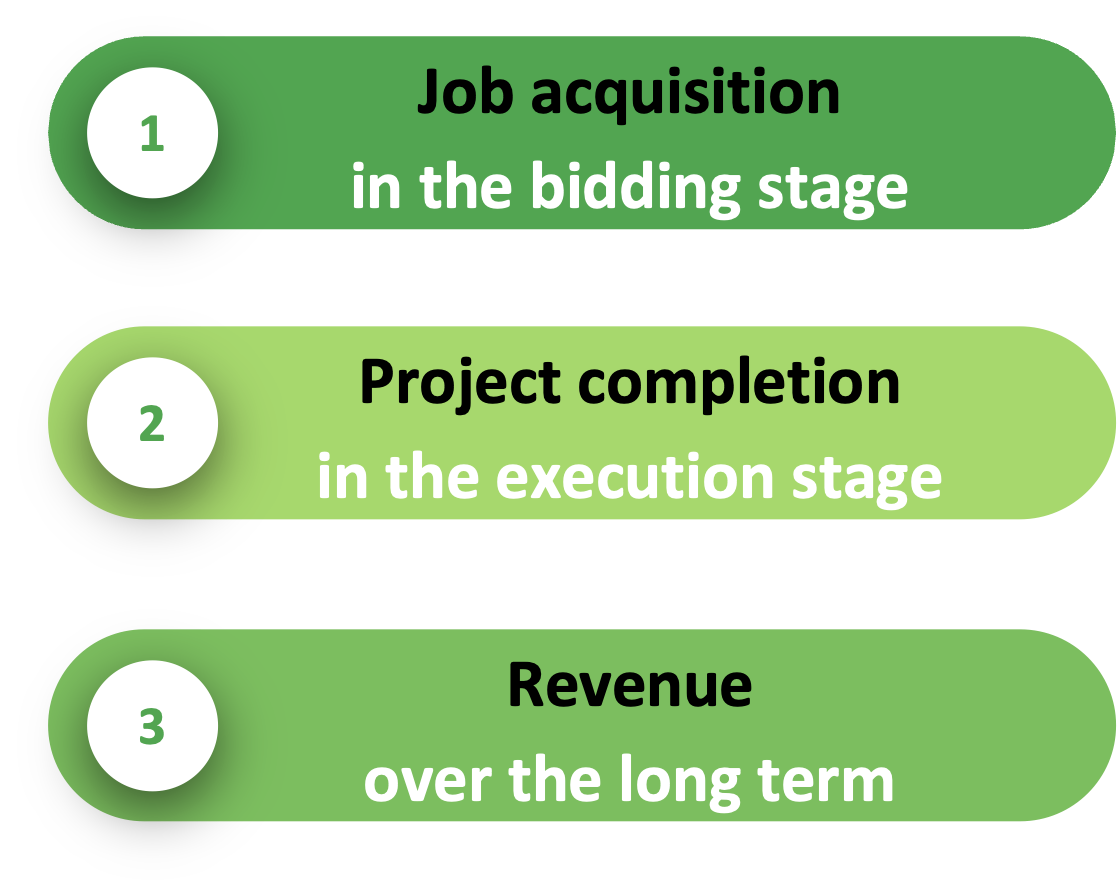
\includegraphics[width=.5\linewidth]{Chapters/images/stages.png}
    \caption{Outcome Measures and Associated (Project) Time Periods}
    \label{stages}
\end{figure}

\paragraph{Bidding Phase Strategies}
Vetting for a job in online freelancing platforms may seem intimidating to many workers, especially to beginners who may be submitting their first few bids. But as \cite{Hong2021-hj} {has} shown, reaching out to clients has a significant and positive impact on a freelancer's chances of procuring a job. Among the workers who do initiate conversations with clients, we consider whether content curation would have an effect on hiring probabilities. At the beginning of this investigation, the use of proposal (bid) templates was still a recommended practice by platforms such as Upwork. Since sending out templated first messages to multiple clients en masse can save time and maximize resource utility, we expected freelancers to leverage the advantages of template use when initiating conversations with clients. 

Since the online gig economy is structured as a reverse auction market, clients are often subject to information asymmetries. In particular, the lack of insight into worker bandwidth may lead to wasted time and effort for the client \cite{Horton2018-eq}. Receiving direct messages from freelancers can help clients overcome such obscurity since the gesture of outreach serves as an indicator for clients to gauge the bandwidth and capacities of a freelancer. While we know that outreach in general has a positive effect on hiring probabilities \cite{Hong2021-hj}, we may expect templated messages to induce the opposite effect: clients might observe that the freelancer has the time, capacity and perhaps even desperation \cite{dunn2020motivation} to find work, but not the resources necessary to personalize the content of their message to target the needs of their individual project. Hence, we can expect clients to hire more freelancers who demonstrate sincerity through individualized content curation in their first outreach message and bid proposal texts:
\newline

\textbf{Hypothesis 1:} During the bidding stage of a project, we posit that
\begin{enumerate} 
  \renewcommand{\labelenumi}{\alph{enumi}.}
    \item Standardizing first message text will \textit{decrease} the probability of winning the bid.
    \item Personalizing bid text to match job description requirements will \textit{increase} the probability of winning the bid.
\end{enumerate}

\paragraph{Execution Phase Strategies}
Due to intense competition in the online labor market \cite{dunn2017digital}, freelancers may feel pressured to respond to client requests as quickly as possible to minimize the chances of the clients noticing and hiring other competitors. However, this may reduce productivity during the execution phase since ``constantly attending to IM \dots may prevent users from performing tasks efficiently'' \cite{Avrahami2004-cd}. Furthermore, the cognitive switching costs accrued by toggling between attending to messages and focusing on work is especially pronounced during the execution stage: ``the time to switch to the message was significantly slower when the notification arrived during the execution phase than either other phase'' \cite{Cutrell2000-ap}. 

The expectation to remain responsive may disrupt freelancers' workflows, allowing clients to interrupt them when completing a task, thereby reducing their working efficiency. Some direct messages may exhibit characteristics of outeraction - communicative processes people use to connect with each other and to manage communication, rather than to information exchange. Outeractions can be especially disruptive because the content of the exchange is unrelated to the freelancer's task at hand: ``time spent on messages and time to resume the search task were both longer when the message was irrelevant than when it was relevant'' \cite{Cutrell2000-ap}. Hence, our second hypothesis examines how personalizing practices during the execution stage, such as responsiveness and accommodating the ``regular hours'' of a client, can affect project completion outcomes:
\newline

\textbf{Hypothesis 2:} During the execution stage, we expect that
\begin{enumerate}
  \renewcommand{\labelenumi}{\alph{enumi}.}
    \item Responding during a standardized period during the day will \textit{improve} the probability of completing a project.
    \item Personalizing response times (increasing responsiveness) will \textit{negatively impact} the probability of completing a project. 
\end{enumerate}

\paragraph{Messaging Techniques \& Revenue}

Outcomes such as award and completion statuses serve to measure the success of various messaging practices at the individual project level. However, to evaluate the impact of these practices over the long term, we must observe a more aggregated measure of the freelancer such as their monthly revenue or earning efficiency. With the exception of a study that found multitasking among Turkers to generate higher income more quickly \cite{Brewster_Fitzpatrick_Cox_Kostakos_Lascau_Gould_Cox_Karmannaya_Brumby_2019}, there's a scarcity of literature available investigating the effects of messaging patterns on freelancer revenue.

We think there is reason to believe that over the long term, standardization can help freelancers generate revenue while personalization will hurt their quantity of earnings because personalizing content for each specific client and always being available for and responsive to clients can be draining and unsustainable over the long term. But on the other hand, the opposite might also hold true: freelancers could adapt to manage their time in a way that they personalize and thrive for each of their projects without experiencing burnout. Thus, we leave the effects of standardization and personalization on revenue as a research question to be examined:
\newline

\noindent\textbf{RQ 3:} How do standardizing and personalizing help or harm revenue?

\section{Research Context \& Methods}
\subsection{Study Platform}
To conduct this study, we obtained data from a corporate partner {(whose specific name will not be disclosed per agreements for data sharing)} that is a leading platform in online freelancing. {Example categories of work include data entry, software development, design, writing, etc.} The dataset we acquired consisted of {2,031,068} messages, from {56,222 } projects posted between January 1, 2010 and March 1, 2010, { involving 58,397 freelancers and 25,480} clients. For each project we observed their associated project descriptions, bid text, messages, as well as timestamps for these artifacts such as the submission and award dates of bids, the completion and payment times, as well as individual message timestamps. We did not impose limitations based on project category. For each stage of a project, we constructed two {separate data frames using this sample}. Observations in the first {frame} consisted of worker-job pairs (or conversations) that incorporated worker-related information such as bid price, bid text, reputation as well as information associated with the job, including project description text, submit date and buyer identification. In a separate freelancer{-level} {frame} we included long term worker-related attributes such as average bidding price and bid volumes.


\subsection{Measures of Key Variables}

We operationalized standardization and personalization in communication depending on the phase of the project. To more precisely capture standardization in the execution phase, we removed freelancers who multitask and work on more than one project at once -- multitaskers represented roughly 12\% of those who were awarded projects.

\paragraph{Bidding Phase Strategies}  
  \setlength\itemsep{1em}

\begin{itemize}
\item \textbf{First Message Standardization:} To measure the extent to which freelancers \textit{standardize} content in a conversation (i.e. worker-job pair) during the initial bidding stage, we calculated the \textit{first-message similarity}. We obtain this measure for a particular conversation by calculating the cosine distance between the freelancer's vectorized \footnote{ The vectorization approach we use is to simply create counters for word occurrences in the messages.} first message in the current project and the vectorized first message of their most recent prior project. Hence, freelancers who use the same set of words across first messages to multiple clients tend to score higher in this measure since they are more likely to employ standardized templates when conducting outreach. 

\item[\ding{46}] {\underline{Example:} If freelancer $F$ uses a template $T$ and sends $T$ in their first message to the clients in both projects $P_1$ and $P_2$ (assuming $P_2$ immediately follows $P_1$), they will receive a measure of 1 for their first message standardization for project $P_2$. But if for their project $P_3$, $F$ sends a  first message that is completely different to the previous two (i.e. no words in the first message of $P_3$ matches those in $T$), then the standardization measure for $P_3$ would be 0.} Since this measure only concerns the first message content sent by the freelancer in each project, it will only be used as an explanatory variable for the bidding stage model.

\item  \textbf{Bid Text Personalization:} To quantify the amount of \textit{personalization} that freelancers employ in the bidding stage, we computed the level of curation in the freelancer's bid text. This measure represents the degree of likeness (again obtained via cosine similarity) between the textual content of a freelancer's bid application and its associated project description post (submitted by the potential employer). Accordingly, freelancers who choose to include words and mirror content from the client's job post are considered to have higher measures of personalization. 
\item[\ding{46}] {\underline{Example:} Freelancer $F$ submits a bid application $B_1$ to project $P_1$. $B_1$ borrows many words from the job posting. Subsequently, $F$ applies to another project $P_2$ with $B_2$, but $B_2$ did not make use of any text from the job description. Freelancer $F$ would have a higher measure of content personalization for $P_1$ than for $P_2$.} Similar to first-message similarity, this variable measures a practice that can only be executed in the bidding stage, and will therefore only be used as a predictor variable for hiring outcomes.
\end{itemize}

\subsubsection{Execution phase strategies}

\begin{itemize}
\setlength\itemsep{1em}
    \item \textbf{Response Time Standardization: }After a freelancer makes it past the selection stage and is awarded the job offer, we look at the effects of qualities such as timing on a freelancer's likelihood of successfully completing a project. In particular, we measure \textit{standardization} in this stage by computing  the schedule regularity of a freelancer within a particular project. 
    {To compute this measure, we first find the standard deviation in the timing of the day for a freelancer's messages across all their projects (this is a freelancer-level measure). But since that measures the variance in schedules, we invert the standard deviation by subtracting it from the total number of seconds in a day to better represent schedule regularity. }
    
    \item[\ding{46}]{\underline{High regularity example:} Freelancer $F$ sent a total of two messages, one at 11:02am and another at 11:12am \footnote{{Note that the day when the messages were sent does not affect this variable as it measures regularity on a daily basis.}}. The standard deviation of $F$'s messages is five minutes, which means that the measure of schedule regularity is quite strong at 23 hours and 55 minutes.} 
    
    \item[\ding{46}] {\underline{Low regularity example:} By contrast, freelancer $G$ sent two messages that are much further apart in the day - one of them at midnight (00:00:00) and another at noon (12:00:00). The standard deviation of of $G$'s messages is six hours, and their schedule regularity is much lower (at 18 hours).} Thus, the smaller the deviation in message sending times, {the less likely that the freelancer compromises their own routines to accommodate clients' timezones or schedules. }

    \item\textbf{Response Time Personalization:} To estimate whether \textit{personalization} affects the likelihood of project completion, we calculated for each freelancer-project pair its \textit{responsiveness}. 
    {First we determine the response gap of a message by calculating the amount of time it takes for a freelancer to respond to a message sent by the client}\footnote{ If an employer sends multiple messages before receiving a response, we consider the response time to be the difference in time between the freelancer's first response and the employer's \textit{first} message that has not yet received a response.}. 
    {Then all we average these response gaps across all messages of the conversation to obtain an aggregated measure at the worker-project level. Once again, we invert this measure by subtracting it from the the total number of seconds in a week so that it embodies responsiveness instead of response times.}
    
    \item[\ding{46}] {\underline{High responsiveness example: } Freelancer $F$ responded to two client messages in project $P$. For the first message they replied back 90 minutes after the client's message while the second response took them 30 minutes. The average response time of freelancer $F$ in project $P$ is very quick at 1 hour, which means that $F$'s average responsiveness in project $P$ is 6 days and 23 hours.}
    
    \item[\ding{46}] {\underline{Low responsiveness example: } Now let's say freelancer $G$ also worked on project $P$, and responded to two client messages for this project as well. Their first reply only took 1 hour but they missed the client's second message and ended up taking 9 days and 23 hours (a total of 239 hours) to respond. So the average response time for freelancer $G$ in project $P$ is much slower (at 10 days, or 240 hours), implying that their responsiveness for project $P$ is much lower at 4 days.}{ Intuitively, freelancers incur shorter gaps when they are being more responsive}, which also demonstrates greater amounts of personalization in terms of message timing.
    
\end{itemize}

\subsection{Outcome Measures and Control Variables}

For measuring success at different stages, we gather the \textbf{job award status} to assess the outcome of the bidding stage, \textbf{project completion status} for the execution stage, and \textbf{overall monthly revenue} to account for long-term earnings. Both award and completion status are binary variables where ``awarded'' or ``complete'' corresponds with 1 while all other statuses (``rejected'', ``incomplete'', or ``pending'') are marked as {0}. Revenue is a dollar amount calculated on a monthly basis, the final value of of revenue per month is normalized with standard scaling.

Beyond these key explanatory variables, we also include other controlled variables: {reputation is measured by whether the worker has received reviews in the past (\textit{had prior reviews}), \textit{bid price} is the amount that the freelancer is proposing to charge for their work (this variable is log-transformed to remove skewedness), \textit{freelancer message count} is the total number of messages the freelancer sends within the project, number of bids won and projects completed account for how many projects the freelancer's has historically being hired for and completed, respectively, and are also log-transformed. All predictor variables are normalized for analysis via standard scaling. In Table 1 we provide descriptive statistics of both key and control variables for each of our models.}

\begin{table}[h!]
\centering
\resizebox{\textwidth}{!} {
\begin{tabular}{lccccccc}
\hline
\textbf{Bidding stage (project-level {frame})} 
& \multicolumn{1}{l}{}                      
& \multicolumn{1}{l}{}                                   
& \multicolumn{1}{l}{}       
& \multicolumn{1}{l}{}       
& \multicolumn{1}{l}{}      
& \multicolumn{1}{l}{} 
& \multicolumn{1}{l}{} \\ \hline
{Measure}                  
& \multicolumn{1}{l} {Mean} & \multicolumn{1}{l}{{Standard Deviation}} & \multicolumn{5}{c}{Correlations} \\ \cline{4-8} 
& \multicolumn{1}{l}{}                      
& \multicolumn{1}{l}{}                                    
& 1                          
& 2                          
& 3                         
& 4                    
& 5 \\ 
\hline
\textit{1. First message standardization} & \ 
.49{4}                                    
& {.344}                                               
& \multicolumn{1}{l}{}       & \multicolumn{1}{l}{}       
& \multicolumn{1}{l}{}      & \multicolumn{1}{l}{} 
& \multicolumn{1}{l}{} \\
\textit{2. Bid text personalization}      
& .128                                   
& {.124}                                               
& \multicolumn{1}{l}{-.106} & \multicolumn{1}{l}{}       
& \multicolumn{1}{l}{}      & \multicolumn{1}{l}{} 
& \multicolumn{1}{l}{} \\
\textit{3. Had prior reviews}             
& .61{1}                                   
& .487                                               
& \multicolumn{1}{l}{.211}  & \multicolumn{1}{l}{-.175} 
& \multicolumn{1}{l}{}      & \multicolumn{1}{l}{} 
& \multicolumn{1}{l}{} \\
\textit{4. Bid price (log)}               
& 5.05                                     
& 1.36                                               
& \multicolumn{1}{l}{.121}  & \multicolumn{1}{l}{.031}  
& \multicolumn{1}{l}{.043} & \multicolumn{1}{l}{} 
& \multicolumn{1}{l}{} \\
\textit{5. Bids won (log)}               
& 2.12
& 1.93                                              
& \multicolumn{1}{l}{{.212}}  & \multicolumn{1}{l}{{-.154}}  
& \multicolumn{1}{l}{{.758}} & \multicolumn{1}{l}{{.078}} 
& \multicolumn{1}{l}{} \\ \hline

\textbf{Execution stage (project-level {frame})}
& \multicolumn{2}{c}{}       & \multicolumn{1}{l}{}       
& \multicolumn{1}{l}{}       & \multicolumn{1}{l}{}      
& \multicolumn{1}{l}{}       \\ \hline

\textit{1. Response time standardization} 
& 7.05e04 & 4.15e03 & & & & &                      \\
\textit{2. Response time personalization} 
& {5.22}e5 & 6.23e05 & -.025 & & & &                      \\
\textit{3. Had prior reviews} 
& .612 & .487 & -.281 & .008 & & &                      \\
\textit{4. Bid price (log)}                        
& 5.06 & 1.36 & .050 & -.021 & 
.043 & &                     \\
\textit{5. Freelancer message count}      & 4.82 & 7.90 & -.082                     & .002                      & .107                     & -.018               \\
\textit{6. Projects completed (log)}
& {4.35} & {1.38} & {-.107} 
& {-.005} & {.251} & {.029} & {.040}
\\ \hline

\textbf{Freelancer - level {frame}}                  
& \multicolumn{1}{l}{} & \multicolumn{1}{l}{}
& \multicolumn{1}{l}{}       & \multicolumn{1}{l}{}       & \multicolumn{1}{l}{}      & \multicolumn{1}{l}{} \\ \hline
\textit{1. Average first message standardization}  & {.472}                                    & .253                                               &                            &                            &                           &                      \\
\textit{2. Average bid text personalization}       & .13{5}                                   & {.100}                                              & -.{189}                     &                            &                           &                      \\
\textit{3. Average response time standardization}  & 7.03e04
& 3.9{8}e03                   
& -.0{75}
& .1{59}                &                           &                      \\
\textit{4. Average response time personalization}  & {5.69e5}                                     & {3.72e04}
& -.01{8}                     
& -.0{77}                
& -.{129}                    &                      \\
\textit{5. Average bid price (log)}       
& 4.{86}                                     
& .8{96}                                            
& .1{66}                     
& -.0{36}                 
& .00{8}               
& -.0{66} \\
\textit{6. Had prior reviews average}              & .63{5}                                    & .4{52}                                              & .2{44}                      & -.2{56}                     & -.237                    & {.119} & {.120}       
\\ \hline
\end{tabular}
}
\caption{Correlations, means and standard deviations of explanatory variables}

\end{table}


\subsection{Statistical Models }
Using separate linear regression models for different stages, we observe the effects of standardization and personalization techniques toward project hire, completion outcomes as well as earnings. When testing the hypotheses about the bidding and execution stages (H1 and H2), we eliminate the possibility that hiring and completion statuses are jointly determined with our explanatory variable by including a project-level fixed effects when running the logistic regression model. This captures time-invariant and job specific properties that might impact the model outcomes, as well as employer-level fixed effects, since there can be only one employer per job. 

The models also include observable worker characteristics that may vary across bids such as reputation status and bid price. At the revenue level (R3), we first ran a regression model that used the four aforementioned strategies {(measured by our key variables)} to predict monthly revenue. Subsequently, we used the two bidding stage measures to predict the total freelancer bidding volume over the three month period to provide further insights for results of the revenue model.

\newpage 
\section{Results}
\crefname{table}{}{} % No prefix for lowercase references
\begin{table}[h!]
\centering
\caption{{ Bidding stage regression model with project fixed effects predicting job awards. }}
\label{bidding}
\begin{tabular}{l c c}
\hline
\begin{tabular}[c]{@{}l@{}}Dependent Variable:\\ \textbf{Job award}\end{tabular} & Coefficient   & Standard Error  \\ \hline
\textit{First message standardization}                                            & -.0{30}1*** & 8.2{3}e-05   \\ \hline
\textit{Bid text personalization}                                                            & .03{58}***  & 2.30e-03   \\ \hline
\textit{Had prior reviews}                                                            & {3.90e-03}***  & {7.72e-04}     \\ \hline
\textit{Bid price (log)}                                                      & -.02{58}*** & 5.{36}e-04   \\ \hline
{\textit{No. bids won (log)}}                                                      & {7.30e-03***} & {2.38e-04}    \\ \hline
Number of observations                                                  & \multicolumn{2}{c}{603,286}    \\ \hline
\multicolumn{3}{c}{*** signifies a p-value \textless .001, errors are clustered by project}           \\ \hline
\end{tabular}
\end{table}
\FloatBarrier
\subsection{{Bidding Strategies' Impacts on Hiring}}
Table \cref{bidding} shows the bidding stage regression results, where we explore the impacts of standardizing and personalizing first messages on the project award outcome (1 is awarded and 0 if not). The coefficients show that increasing standardization during the bidding stage hurts a freelancer's hiring probabilities, {thereby supporting H1a. Specifically, standardizing first message content by one standard of deviation reduces their winning probabilities by .03\%. Meanwhile, personalizing and curating the contents of a bid proposal based on the job posts increases their chances of winning the project (which is in alignment with H1b), but only slightly -- personalizing bids by one standard of deviation improves award probability by .036\%. } 

Note that we also controlled for freelancers' bid prices (which were log transformed after adding one since the log of zero is undefined),  reputation -- measured via the dummy variable \textit{had prior reviews}, which represents whether the freelancer has received a rating for their work in the past, and a historical bidding success variable -- the number of bids the freelancer won prior to the current project. We intentionally chose to not include actual rating values because the majority of ratings are positive and most jobs do not end up receiving reviews - their inclusion would cause an inflated measure of reputation. As one would expect, {having previously won bids and} reviews {to showcase on the profile} is favorable for hiring, whereas bidding at a higher price harms hiring probabilities {of a freelancer}. 

\begin{table}[h]
\centering
\caption{Execution stage regression with project fixed-effects predicting job completions.}
\label{execution_table}
\begin{tabular}{lcc}
\hline
\begin{tabular}[c]{@{}l@{}}Dependent Variable:\\ \textbf{Job completion}\end{tabular} 

& Coefficient   & Standard Error \\ \hline
\textit{Response time standardization}                                                             & {1.15e-07}  & 1.1{6}e-07 \\ \hline
\textit{Response time personalization}                                                                   & -9.{10}e-0{9}*** & {1.63}e-09  \\ \hline
\textit{Had prior reviews}                                                                    & {5.90}e-03***  & {2.01}e-03 \\ \hline
\textit{Bid price (log)}                                                              & -1.2{7}e-02*** & 1.0{3}e-03 \\ \hline
\textit{Freelancer message count}                                                        & 8.{1}6e-03***  & 5.{52}e-04\\ \hline
{\textit{No. completed projects} }
& {1.36e-03 .}  & {7.33e-04} \\ \hline
Number of observations                                                          & \multicolumn{2}{c }{1{10,797}}    \\ \hline
\multicolumn{3}{ c }{*** signifies a p-value \textless .001 and . denotes a p-value < .1}
 \\ \multicolumn{3}{ c }{Errors are again clustered by project} \\ \hline
\end{tabular}
\end{table}

\subsection{{Execution Strategies' Effects on Completion}}
Table \cref{execution_table} shows our results for the execution stage model, where we explore the impacts of standardizing or personalizing responses time on the job completion.
In this stage, we observe that { in alignment with H1a, being online at regular hours of the day has a small and positive but insignificant effect on a} freelancer's chances of completing a project.
Meanwhile, being highly responsive to client messages (the personalization technique) significantly hurts completion, {which is in agreement with H2b, but the effect is negligible}. 

Reputation and bid prices have a similar effect as in the bidding stage model. This suggests that reputable freelancers have higher chances of satisfying the demands of a client. Workers who demand higher payments will have a harder time gaining approval from their clients, since more costly payments {will likely} lead to increased expectations for work quality. {Having received ratings for prior work is positively correlated as well.} We also controlled for the number of messages that a freelancer sends within the project, since {message frequency} will have a consequential impact on the variance/regularity of a worker's messaging schedule, {and found that messaging more positively impacts completion probabilities. Meanwhile, having successfully completed projects slightly helps execution of the current one.}

\begin{table}[h]
\centering
\caption{ Freelancer-level regression predicting monthly revenue with monthly fixed effects.}
\label{long_term}
\begin{tabular}{l c c}
\hline
\begin{tabular}[c]{@{}l@{}}Dependent Variable:\\ \textbf{Monthly revenue}\end{tabular}  
& \multicolumn{1}{l }{Coefficient}          & \multicolumn{1}{l }{{Standard Err.}}  \\ \hline
\textit{{Avg. first msg. standardization}}                                           & {.123}*** & {3.23}e-02                     \\ \hline
\textit{{Avg. bid text personalization}}                                       & -.1{46}** & 3.{6}2e-02     \\ \hline
\textit{{Avg. response time standardization}}                                  & -{1.18e-06} & 1.{37}e-06 \\ \hline
\textit{{Avg. response time personalization}}                                  & -{1.52e-07} & {1.61e-07}    \\ \hline
\textit{Avg. bid price}                                                      & .2{17}*** & 1.{22}e-02  \\ \hline
\textit{Had prior reviews average} 
& .36{0}*** & 1.{61}e-02    \\ \hline
\textit{Number of observations}                                                 & \multicolumn{2}{c}{161{49}}                                                               \\ \hline
\multicolumn{3}{ c }{\begin{tabular}[c]{@{}c@{}}\text{*** signifies a p-value \textless .001, ** denotes a p-value \textless .01}\\ \text{Errors are clustered by month}\end{tabular}} \\ \hline
\end{tabular}
\end{table}

\subsection{{Long-term Strategies' Impact on Earnings}}
Our earnings model uses a freelancer-level instead of a project-level {frame} to capture revenue from all jobs of a month. Here we measure the effects of the same two pairs of standardization and personalization techniques above {to investigate the question posed in R3}. The four measurements are aggregated for each freelancer {frame} by averaging, and fixed effects are added to account for time variance. 

Table \cref{long_term} reveals that only messaging practices in the bidding stage had significant impacts on overall revenue. Specifically, standardization has a positive effect on revenue {- increasing content standardization by one standard of deviation results in a .12\% growth in monthly revenue,} likely because it enables workers to submit more bids. {Meanwhile} bid personalization no longer offers the same enhancing effects it had at the project level. {In fact, personalizing bid content by one standard of deviation can cost workers .15\% of their monthly revenue}. Reputation continues to impact success in the same ways as before, and bid higher for individual projects naturally increases overall freelancer earnings.

{To test our hypothesis that the inverted effects of content standardization is related to how} it enables workers to take on larger volumes of work, we ran an additional model using bid volume as the dependent variable. {The results (Table \cref{bid_volume}) show that increasing first message standardization by one standard of deviation} during bidding {can allow workers to apply to 36.6\% more projects}, {thereby} increasing their total earnings in the market.

\begin{table}[h]
\centering
\caption{Freelancer-level regression predicting bid volume with monthly fixed effects.}
\label{bid_volume}
\begin{tabular}{ l c c}
\hline
\begin{tabular}[c]{@{}l@{}}Dependent Variable:\\ \textbf{Bid volume}\end{tabular}          & \multicolumn{1}{l}{Coefficient}         & \multicolumn{1}{l}{Standard Error}  \\ \hline
\textit{{Avg. first msg. standardization}}                                             & {36.6}*** & {4.64}                   \\ \hline
\textit{{Avg. bid text personalization}}                                         & {-8.90 .}  & {4.45} \\ \hline
\textit{{Avg. bid price (log)}} 
& {5.79}*** & {.720}  \\ \hline
\textit{Got reviews}                                                              & {28.0}*** & {2.64}  \\ \hline
\text{Number of observations}                                                   & \multicolumn{2}{c}{161{49}}                                                             \\ \hline
\multicolumn{3}{c}{\begin{tabular}[c]{@{}c@{}}*** signifies a p-value \textless .001 and . denotes a p-value \textless .1\\ Errors are clustered by month\end{tabular}} \\ \hline
\end{tabular}
\end{table}

\section{Discussion}
We examined the effects of standardizing versus personalizing communication practices on individual project success and monthly freelancer earnings. Our first set of findings confirmed that during the bidding stage, content standardization negatively associates with hiring rates {(H1a)} while personalization has a positive {correlation (H1b)}. From this, we can infer that template use in the initial bidding stage may leave a negative impression with employers by signifying that the associated project is only one among many from the worker's perspective. Relatedly, borrowing and incorporating words and phrases from the client's own description of the project appears to have a favorable effect on clients, perhaps conveying worker sincerity and attentiveness. This suggests that when crafting job proposals (i.e. bid applications), workers may want to carefully read and curate their writing to match the individual job requirements, instead of copying and pasting from templates. Or, as Upwork recommends -- ``Don't use a proposal template'' \cite{noauthor_undated-wy}.

However, our analysis of monthly revenue showed that over the long term, content standardization contributes to higher worker earnings, revealing a trade-off between project-level success and long term earning efficiency. To interpret potential mechanisms behind this effect, we examined the effects of the two strategies on bid volume (Table \ref{bid_volume}), which unveiled that using standardized proposal templates enabled workers to submit more bid applications, thereby indirectly contributing to higher monthly earnings. This tradeoff between standardization over the long term and personalization at the individual project level suggests that a worker should keep in mind their broader, long-term career goals while attending to minute and specific details {of individual} projects.


Once a freelancer begins working on the project, a fear of losing the gig might cause them to be overly responsive to a particular employer. 
Our results from the execution stage (Table \cref{execution_table}) indicate that this reactive communication approach is negatively associated with project completion {(H2b)}. 
This resonates with prior literature on instant messaging, which also found that always being highly responsive to messages in work-related conversations harms workers' abilities to stay on task \cite{Avrahami2004-cd}. Although our analysis does not indicate that response time standardization correlates significantly with long-term earnings, this null result may be due to other hidden characteristics, omitted from our model.

In place of instant replies, freelancers might consider a more proactive form of time-management where they adhere to a consistent daily work schedule and respond only at appropriate times within their own working hours. Naturally, some freelancers may only participate in the online labor market on a part-time basis (referred to by some as \textit{casual earners}), while others are more professionally engaged (including those who are \textit{financially strapped}) \cite{manyika2016independent}. Regardless of a freelancer's online or offline employment status, there is reason to believe that having a consistent work schedule and an increased awareness of time will only benefit a workers' financial and mental well-beings over the long run.


To summarize, our results suggest that freelancers attempting increase their odds of winning a project can consider personalizing the content of their bid applications to cater toward client needs, those who have secured jobs can increase their chances of completion {if they refrain from instantly responding to client messages. Workers seeking to increase monthly earnings might consider bidding for projects, which can be achieved through the use of standardized bid proposal templates.} Across all of our models, having reviews on a freelancer's profile positively impacts success, implying that workers seeking to thrive in the online environment may also benefit from image and reputation management.

\subsection{Design Implications}

Given these empirical findings, we propose design recommendations for tools that seek to support gig workers in their various endeavors. Since {temporal responsiveness was shown to be harmful toward project completion success,} designers might consider mechanisms that {help workers stay focused and on task}. This may take the form of an application or plugin, which may adopt features akin to {those found in focus and productivity apps. Current platforms such as Upwork may also want to reconsider the inclusion of responsiveness \footnote{https://support.upwork.com/hc/en-us/articles/211062968-My-Stats} in worker profiles, since a worker's ability to respond to messages quickly might negatively impact their ability to finish a project.}

To make bid personalization easier for workers, tool designers might attempt to use natural-language processing (NLP) methods to extract job requirements from project descriptions and surface them to workers in a more readable fashion. Note that even though current systems do have skill tags that allow clients to clearly define the scope of their project, we can expect many jobs to have unique specifications that cannot be captured by the limited options of a skill tag drop-down. Finally, for workers with relatively low monthly revenues, tools {can} provide reminders\ to motivate them to submit more bids and {so that they may} maximize their hiring probabilities and work volumes.

%\addtocontents{toc}{\protect\clearpage} % <--- just debug stuff, ignore
\chapter{Aligning Multi-Stakeholder Policy \& Tech Preferences  via  Codesign}

Beyond an understanding of scalable communication strategies in online freelancers, it is imperative to also understand worker challenges and strategies across gig work platforms and domains. 
Prior works in the domain have extensively documented the downstream impacts of unregulated space of gig labor platforms on workers (\cite{schulze2022algorithmic, li2022well, arnoldi2021mapping}) across platforms --- ridesharing \cite{regulate, gender, alienated}, freelancing \cite{precarity, privacy, uncertainty}, crowdwork \cite{alienated, crowd_inv}, carework \cite{beyond, strangers}).  For instance, in their seminal work examining job quality in gig work, Wood et. al. described how platformic control causes workers to have weak structural power compared to clients, which results in burnout \cite{good}. Yao et. al. found that while social media groups enabled workers to share experiential knowledge amongst one another, they fell short in building a collective identity among workers since strategic information-sharing could harm an individual worker's comparative advantage \cite{atom}. Howard investigated how labor laws apply in non-standard gig work arrangements, underscoring the health and safety risks involved for workers in such environments \cite{Howard2017-wd}. 
However, such works have yet to explore the prospective future solutions for mitigating cross-domain challenges in gig work. In this chapter, I covered how we leveraged speed-dating codesign sessions with multiple stakeholder groups to approach practical solutions for addressing issues affecting gig workers across domains. 

Recent bodies of work within HCI increasingly urge and pursue the design of systems from a worker-centered perspective \cite{Yang2020-dg,zhang2022algmanagement,Park2022-qy}. As a first step in this direction, Zhang et. al. codesigned alternative platform futures with workers to minimize the impact of algorithmic management on well-being \cite{zhang2022algmanagement}. In their research agenda, Ashford et. al. drew from organizational behavior theory to delineate potential behaviors that individual workers can capitalize on to thrive in the new world of work \cite{Ashford2018-dw}. While these studies focus on worker-driven solutions, improving gig worker conditions requires the active involvement of and collaboration with multiple stakeholder groups \cite{Forlizzi2018-eb, goods2019your}. Expertise of regulators and lawmakers are required to craft and enforce mandates and labor regulations that govern the gig economy \cite{bates2021lessons, Dubal2019-qi}, support from platforms is crucial to implement programs and engage in co-regulation \cite{cannon2014framework, healy2020sceptics}, and worker input is indispensable to designing legal and platformic changes that engender practical and productive impact \cite{organizing, lord2022sustainability}. 

Our work involved a diverse set of stakeholders, and by leveraging the speed dating method, we collaborated with participants from within the United States to brainstorm, develop and assess a wide range of service, policy and technological interventions for addressing the various social, financial and physical challenges of gig work \cite{Davidoff2007-fq}. The hidden costs and challenges emerging from such past bodies of work, combined with themes uncovered from local workshops and news articles, informed the construction of scenarios for our workshops. During the codesign sessions, speed dating allowed us to incorporate reported issues into scenarios accompanied by provocative questions and solutions, empowering us to 1.) learn latent social needs and boundaries of stakeholders and 2.) imagine and evaluate solutions without the high efforts of implementation. 
% To help participants kick off the process of idea generation, we seeded the solution space with interventions that are implementable by platforms, lawmakers, or workers themselves.
% To evaluate the feasibility of solutions in practice, we recruited participants from the same three stakeholder groups.
In conducting these workshops, we sought to answer the following research questions:

\textbf{Research questions: }
\begin{enumerate}
\item What incentives, preferences and deterrents do stakeholders have in supporting and implementing solutions for improving gig worker well-being?
\item What are the most desirable and feasible changes for improving challenges present in gig work?
\end{enumerate}

% We conducted a series of codesign workshops with 20 participants (8 workers, 7 local regulators and 5 platform-side employees) within the United states. 
% Our workshops include an exercise ranking potential future solutions and follow-up questions regarding rationales behind such rankings, allowing us to share key quantitative and qualitative insights from regulators, platform practitioners as well as the gig workforce at large. 
Our multi-stakeholder workshops allowed us to share key quantitative and qualitative insights from regulators, platform practitioners and the gig workforce at large, revealing details about shared worker struggles, desired benefits and steps that stakeholders can take to turn imagined futures into reality. Thus, we make unique research contributions by 1.) presenting improvements to the gig work condition that are acceptable to multiple stakeholders groups and 2.) offering a discussion of how stakeholders can contribute to solutions and interventions. Through this endeavor, we hope to contribute to a future gig workplace that tracks and improves workers' physical, financial and social well being, so as to approach more equitable and inclusive gig platforms and communities. 

\section{Related Works}
One way to segment gig platforms into domains is to consider the type of services provided: app work (e.g. Uber, DoorDash, TaskRabbit), crowdwork (e.g. Amazon Mechanical Turk), and capital platform work (e.g. Airbnb, Etsy) \cite{Duggan2020-qh}. A similar categorization sections platforms based on the physical or remote nature of the labor, with the former consisting of location-dependent labor (e.g. transport, food delivery, furniture assembly) and the latter comprising of digital services such as software development or logo design \cite{Huws2016-vv}. At the start, we focused primarily on app workers performing physical tasks, but found capital platform workers to share many of the same risks and challenges after reviewing relevant literature and articles. Thus, our workshops aim to address the various social, financial and power struggles as well as health and physical risks endemic to these two forms of gig work. In the following, we summarize five major shortcomings of gig work explored in past studies that informed our workshop design.


\subsection{Existing Risks and Challenges}\label{challenges}

\paragraph{Missing Employment Benefits} 
Although gig work offers more flexible work hours, limited employment benefits forces workers to complete additional hours of unpaid labor \cite{anwar2022faux}.
While many workers prefer to keep their legal classification as independent contractors for the associated flexibilities (e.g. no employer attachments), the lack of a formal employment arrangement costs them many benefits and protections, including wage guarantees, workers' compensation, unemployment insurance, healthy and safe work spaces, and the right to unionization \cite{Dubal2019-qi}. The deprivation of workers' rights and protections that contractors experience (which especially impoverishes the mental health of working mothers \cite{kirwin2022working}) has been longstanding, with accounts dating back to at least 2002 \cite{ilo2002resolution}.

In an effort to avoid employment regulations, many gig platforms leverage workers' desires to remain contractors as an argument in court to avoid responsibilities of providing employee benefits. This argument for platforms is frequently used in trials since as early as 2017, after which more than 100 such US lawsuits have been filed against Uber regarding driver misclassifications, with many more appearing across other platforms and nations \cite{employment, category}. To continue exploiting the legal loophole in employment classifications, gig platforms have spent hundreds of millions to lobby for the ballot measure Prop 22 in the summer of 2021 \cite{conger2021judge}. Presently, how workers should be classified remains an ongoing debate -- the control and economic realities tests that serve to distinguish between employees and independent contractors both lead to indeterminate results when applied to rideshare drivers, and different courts'  interpretations of labor laws vary across statutes \cite{category, harris2015proposal}.

\paragraph{Income Instability}
Gig workers also suffer from a lack of financial stability induced by job precarity and the temporary nature of contractual work \cite{anwar2020precarity}. In their study evaluating the job quality of gigs, Wood et. al. identified {how} algorithmic management of workers cause{s} financial instability, social isolation as well as overwork and exhaustion \cite{good}. The combination of low pay, high job insecurity, long working hours induces a high sense of precarity among gig workers \cite{Dubal2017-bj,Hua2018-qx,precarity,Webster2016-gi,Vosko2006-ec}. One major contributor to the income instability of gig workers is seasonality, endangering the financial security of part-time gig workers. For instance, work in sports has always been characterized as precarious and seasonal, and the suspension of several major sports during the pandemic has intensified such impacts \cite{javits2022gig, sheptak2020sport}. Ravenelle et al. also identified increased vulnerabilities of gig workers during the pandemic, finding knowledge, sociological, and temporal/financial hurdles that prevent their access to unemployment assistance \cite{ravenelle2021side}.

\paragraph{Minimal Access to Working Necessities}
The growing prevalence of gig work probes at previously unexplored social barriers, highlighting inadequacies in our public infrastructure. In New York City, exploitative labor practices induced by platforms and public infrastructure subject food couriers to dangerous working conditions, leading to a local labor union of cyclists in 2019 -- \textit{Los Deliveristas Unidos} \cite{geschwindt2022biking}. Based on the lived experiences of its constituent deliveristas, the grassroots collective formed a list of five demands surrounding working conditions, including a right to 1.) free public bathroom access 2.) physical public space for eating, resting and protection from harsh weather conditions 3.) hazard pay for work performed that involve physical hardships (e.g. the COVID-19 pandemic) and 4.) protections from e-bike robberies, wage theft and health and safety hazards. While the city council passed a bill last year to ensure bathroom access for workers \cite{nycbill}, enforcement is difficult and deliveristas still report instances of restaurants who restrict bathroom access  \cite{bathroomreport}.

\paragraph{Safety Concerns}
Without proper employment classification, gig workers do not enjoy the regulated safety assets provided to traditional workers (e.g. worker's compensation, health insurance, and unemployment insurance, among other laws and regulations) \cite{boundary, abraham2017measuring, kuhn2021human}. Unfortunately, the non-standard nature of many gig work arrangements raises occupational health and safety risks, increasing scholarly, legal, and societal concern \cite{orr2022necrocapitalism, Howard2017-wd, Almoqbel2019-in}. For instance, Ferrie et al. found that poor mental health outcomes can result from sudden unemployment \cite{Ferrie1998-th}, and by 2006, Virtanen et al.'s review of 27 case studies revealed a solid association between temporary employment and morbidity \cite{Virtanen2005-jp}. Over the past five years, the Markup has tracked a total of 361 ride-hail and delivery drivers as victims of carjackings or attempted carjackings \cite{Kerr_undated-zw}.

Underlying drivers' safety are factors that disincentivize them to self-protect. Almoqbel and Wohn uncovered that platforms' rating systems to prevent drivers from engaging in protective behaviors (e.g. using dash cams) due to passengers' discomfort around monitoring (which lead to poor reviews); they further found drivers to share safety resources, vent about passengers, and coordinate informal union activities in online forums \cite{Almoqbel2019-in}. Beyond physical attacks, Bajwa et. al. discussed how precarity, occupational and platform-based vulnerabilities can cause psychological distress, increased risk for traffic accidents and musculoskeletal injuries, as well as work-induced stress, respectively \cite{Bajwa2018-gy}. From the  perspective of international law, Howard discussed how legal misclassifications cause a loss of protections and benefits for workers across the globe \cite{Howard2017-wd}.


\paragraph{Missing Collective Action Power}
The design and structure of online labor platforms creates unique challenges such as information asymmetries and power imbalances between workers and clients, giving rise to the platformic control and algorithmic management \cite{Lampinen2018-sv,Jarrahi2019-if, precarity, platform_manage,Gray2019-ue, power, Rosenblat_Stark_2016}. 
Such dynamics disincentivize workers from engaging in collectivism due to fears of losing competitive advantages \cite{atom}. Furthermore, the lack of physical workspaces prevents workers from forming collectively identifies and protesting inequities \cite{chesta2019labour, calacci2022organizing}, while antitrust and employment laws legally prevent them from performing such collective actions \cite{anwar2020precarity, paul2019fissuring}. It is also notable to mention that migrant workers comprise a growing portion of the platform labor market, but legal restrictions make it difficult for them to engage in union activities or benefit from national welfare systems \cite{van2020migration}.

To acquire more workplace gains and protections, workers can engage in collective labor activities. But as Yao et. al. and Johnston et. al. find, barriers such as geographic dispersal, individualistic nature of gig work, and platforms' opposition to worker organization, all prevent the building of a collective, group agency \cite{atom, organizing}. Furthermore, ``antiquated notions of collective bargaining \dots surrounding the gig economy'' may not prove useful in the modern digital workforce \cite{organizing}. Meanwhile, Khovanskaya et. al. leveraged historical insights from mid-20th century labor unions toward management to inform how contemporary data-driven worker advocacy can bring workers together over shared concerns and raise public awareness of working conditions, instead of engaging in bureaucratic negotiations with platforms \cite{Khovanskaya2019-xo}. But as Graham et. al. points out, there is a dearth of counterhegemonic research efforts particular to the gig economy that support the ``building of alternatives, outrage, conflict, and worker organization'', a gap that we hope to help fill \cite{graham2018towards, outsidetheboss}.

\subsection{Design Efforts to Study Worker Well-being}
Early efforts to combat algorithmic management arose in contexts of crowdwork (Amazon Mechanical Turk), rideshare driving, and food couriering. The pioneering piece along this line of work centered Turkopticon, a widely-adopted browser plug-in that overlays its requester/employer-reviewing features on top of the AMT site to resist minimal wages, low quality work, and unfair job rejections (a.k.a. wage theft). In the author's own words, the system aimed to ``make questions of work conditions visible among technologists, policy makers, and the media'' \cite{irani2013turkopticon}. A companion tool Dynamo was developed subsequently to facilitate collective organization action among AMT workers \cite{salehi2015we}. A ``social sensing'' probe developed by You et. al. collected and shared personal health data of rideshare drivers with their significant others to promote well-being awareness (especially related to long working hours) and motivate behavioral changes \cite{you2021go}. Zhang et. al. leveraged algorithmic imaginaries to expand participants' current understandings of algorithms so as to generate alternative futures that actually support workers' needs \cite{zhang2022algmanagement}. In \cite{bates2021lessons}, Bates et. al. hosted two rounds of co-design workshops with gig cycle couriers in the U.K. to identify challenges in their working conditions and ideate alternative solutions. Codesign has also been used to unearth the accounts of essential workers such as airport janitorial staff \cite{kang2022stories}. Finally, Alvarez de la Vega, et al. used design fiction (informed by prior literature) in focus groups to discover potential design opportunities for improving the well-being of online freelancers \cite{alvarez2022design}.

These studies all took a worker-centered focus to empower and highlight the voices of underserved workers. We expand beyond workers to capture the opinions of three distinct but relevant stakeholder groups, so that these involved parties may take part in constructing a brighter and improved gig work future. In particular, we hope our findings help policymakers make well-informed decisions when establishing new regulations to protect worker rights, as well as the media and public at large to exert pressure on platforms to implement worker-centered changes, benefits and programs.

\subsection{Multi-Stakeholder \& Solution-Centered Approach}

While the challenges that gig workers face are well-studied, few investigations have taken a holistic perspective to examine how adjacent stakeholders such as platform-side designers or policymakers can play a role in alleviating such constraints. 
By asking our participants to generate and rank solutions to these issues, we aimed to identify the most desired and practical improvements for addressing the challenges present in gig work (RQ2). As Howard identified in their commentary, the key question of who should be held responsible for providing various job protections has yet to be answered \cite{Howard2017-wd}, so we directly asked stakeholders about who should bring forth change (\ref{procedures}) and probed their solution rankings with follow-up questions surrounding underlying incentives and constraints (RQ1).
By eliciting such preferences and limitations, our workshops goes beyond worker perspectives to also explore unmet needs of platforms and policymakers, so as to help maximize their ability to support gig workers as advocates. 
Sociologists identified these three groups as key stakeholders of the gig economy \cite{vallas2020platforms}, and our simultaneous engagement with all three ensures that the solutions arising from our workshops are acceptable to and welcomed by multiple involved parties. 
In particular, we encouraged participates to generate their own solutions as a means of negotiating for potential futures that they find the most suitable. 
After all, many factors that harm worker well-being (e.g. legal misclassifcation, algorithmic management) can only be mitigated with solutions at systemic as well as cultural levels, and such changes require the active collaboration and involvement of lawmakers, platform designers, gig workers, as well as the public at large.

\newpage
\section{Methods}
\FloatBarrier
\begin{table}[h!]
\centering
\caption{Workshop IDs \& Participant Summaries}
\label{tab:participants}
\resizebox{\textwidth}{!} {
\begin{tabular}{|c|l|c|p{7cm}|}
\hline
\textbf{Workshop ID} & \textbf{Stakeholder Group} & \multicolumn{1}{l|}{\textbf{\# Participants}} & \textbf{Relevant experience} \\ \hline
R1 & Regulators/Advocates & 3 & Manager at DHS; Director of community management at National Council of Jewish Women; intern analyst to director; \\ \hline
P1 & Platform employees & 2 & Executive recruiter at a major rideshare organization; Product designer and an ex-employee of multiple e-commerce platforms \\ \hline
W1 & Gig workers & 3 & 1 deliverer and 1 driver for a popular food delivery platform; nurse at a healthcare company; \\ \hline
R2 & Regulators/Advocates & 2 & Director of Mobility Dept for local city; Professor in organizational behavior and public policy \\ \hline
W2 & Gig workers & 5 & Full time food courier of 1.5 years; freelancer at a platform for matching local labor to demand; IT freelancer \\ \hline
R3 & Regulators & 2 & Local councilperson; Professor of Cyber Law, Policy, and Security \\ \hline
P2 & Platform employees & 2 & Product manager at a platform for matching local labor to demand; Program lead at a rideshare platform \\ \hline
P3 & Platform employee & 1 & Employee at a popular food delivery platform \\ \hline
\end{tabular}
}
 
\end{table} 
\FloatBarrier

\subsection{Recruitment and Participants} \label{recruit}
Our participant pool consisted of three stakeholder groups: gig workers, local regulators and members of various public service organizations, as well as employees from popular gig work platforms, who were chosen because they represent the groups that can actively become involved in solutions for improving gig worker well-being, independently or collaboratively. Gig workers can develop and practice their own strategies, policy-makers can enact laws to restrict  how platforms affect workers, platform employees can modify features to improve gig worker well-being, and together they can drive forth systemic changes that bring us closer to healthy and productive gig communities.

We recruited a total of 20 unique participants across 8 workshops. The seven participants from the regulator/advocates group were reached through contacts from the Pittsburgh-based research institute Metro21, and consisted of individuals who self-identified as regulators or worker advocates from local organizations such as the Department of Human Services and United Way. While not all of our regulator participants are actively involved in policy-making (some study public policy while others work for government agencies), we did recruit one councilperson. The eight gig workers responded to our recruitment posts on Reddit and included individuals who made earnings on popular ridesharing or food delivery apps. The last group consisted of five platform employees (e.g. product designers, managers, and engineers) whom we contacted through a combination of Reddit posts and LinkedIn direct messages. Participants selection was based on responses to a pre-screen survey, which asked for affiliated organizations and engagement with gig work(ers). Table \ref{tab:participants} summarizes the workshop participants and their relevant expertise, in chronological order of workshops dates.
\subsection{Study Design} \label{procedures}
\paragraph{Speed Dating}
As the nature of gig work probes at previously unexplored social boundaries (e.g. traditional workers typically do not bear responsibility for consumers' physical or food safety), we require alternative methods for examining workers' needs, as well as to discover the social and cultural barriers that gig work pushes at, which are not yet well understood \cite{Davidoff2007-fq,Zimmerman2017-rq}.
% Because the issues of poor gig work conditions has not yet faced widespread public scrutiny, 
Toward this end, we leveraged speed dating, a method that involved presenting pressing issues (design opportunities) and provocative alternative futures (design concepts) to multiple stakeholders in rapid sequence, enabling us to uncover their latent needs, desires, fears and dreams. 
Unlike romantic speed dating, where the goal is to pair potential couples, the technique strives to match gig work issues to potential solutions. 
Speed dating has been utilized in a variety of domains (e.g. attention management \cite{chou2022because}, AI ethics checklists \cite{madaio2020co} smart homes \cite{jin2022exploring}) to rapidly explore of concepts/solutions to issues without needing to implement the proposed technologies \cite{Davidoff2007-fq}. 
% In accordance with the method, we 
% To elicit such desiderata and aversions

Most similar to our contexts, Dillahunt et. al. found speed dating effective in identifying concepts for addressing needs of underserved job seekers \cite{Dillahunt2018-ia}. 
Following their study design, we presented to participants a series of issues that gig workers face, but did not pair each issue with a tool/design concept in the same way. 
Instead, we offered a list of alternative futures (and encouraged participants to generate their own solutions) to broaden the horizon of imagined possibilities. 
% By gauging the reactions of participants toward proposed concepts, we can match relevant issues and needs to potential future solutions. 
While parts of our study design drew inspiration from \cite{Dillahunt2018-ia}, we center our work around gig workers instead of underserved job seekers, and expand the pool of imagined solutions by incorporating the voices of diverse stakeholder groups. 

\paragraph{Scenario Construction}
Initially, we generated ten scenario stories and subsequently solicited the critique of other researchers working in the space of supporting gig workers to help us finalize a problem space comprising five scenarios (see Table \ref{tab:scenarios}).
The scenarios were developed based on challenges outlined in relevant literature as well as pressing issues that received press coverage. In particular, the fourth \cite{Al_Jazeera2022-vz} and fifth \cite{noauthor_undated-xr} scenarios were conceived based on accounts of stories of worker situations covered in the respective articles. Each scenario maps back to the respective paragraph in 
\ref{challenges}.
To avoid promoting ``blue-sky'' thinking, which (as Harrington et. al. pointed out \cite{harrington2019deconstructing}) may lead to frustration for the very population we intend to serve, the authors collectively generated ideas ahead of time to prepopulate the solution space (which consisted of ideas implementable by each of the three involved stakeholder groups to avoid imbuing our opinions on who should hold responsibility), so as to help participants brainstorm.
% -- a full list of pre-generated solutions can be found in Table \ref{tab:solutions} of the Appendix. 
% The pre-generated solution space consisted of ideas implementable by each of the three stakeholder groups we involved so as to avoid imbuing the research team's opinions on who should hold responsibility.

Though all scenario characters were fictitious, the first three were inspired by concerns expressed during a local workshop organized by the National Council of Jewish Women, which explored the hidden costs of gig work. The fourth \cite{Al_Jazeera2022-vz} and fifth \cite{noauthor_undated-xr} scenarios were based on accounts of stories of worker situations covered in the respective articles. All five scenarios represent prevalent issues gig workers face today: missing employee benefits, financial instability, a lack of essential working necessities, safety issues and workers' minimized ability to take collective action. With the exception of the persona in Scenario 3, who reflects the common characteristics of food deliverers (i.e. male, young, and of an immigrant background \cite{ma2022brush}), the demographics of characters are intentionally non-representative of the general gig worker population to encourage the consideration of marginalized workers (women, elders, etc.), who often face issues such as bias, harassment, and pay gaps, all of which intersect with algorithmic control \cite{ma2022brush, anjali2021watched, foong2021understanding, foong2018women, jahanbakhsh2020experimental}.

\FloatBarrier
\begin{table}[h!]
  \centering
   \caption{Problem Space: Scenario Summaries}
    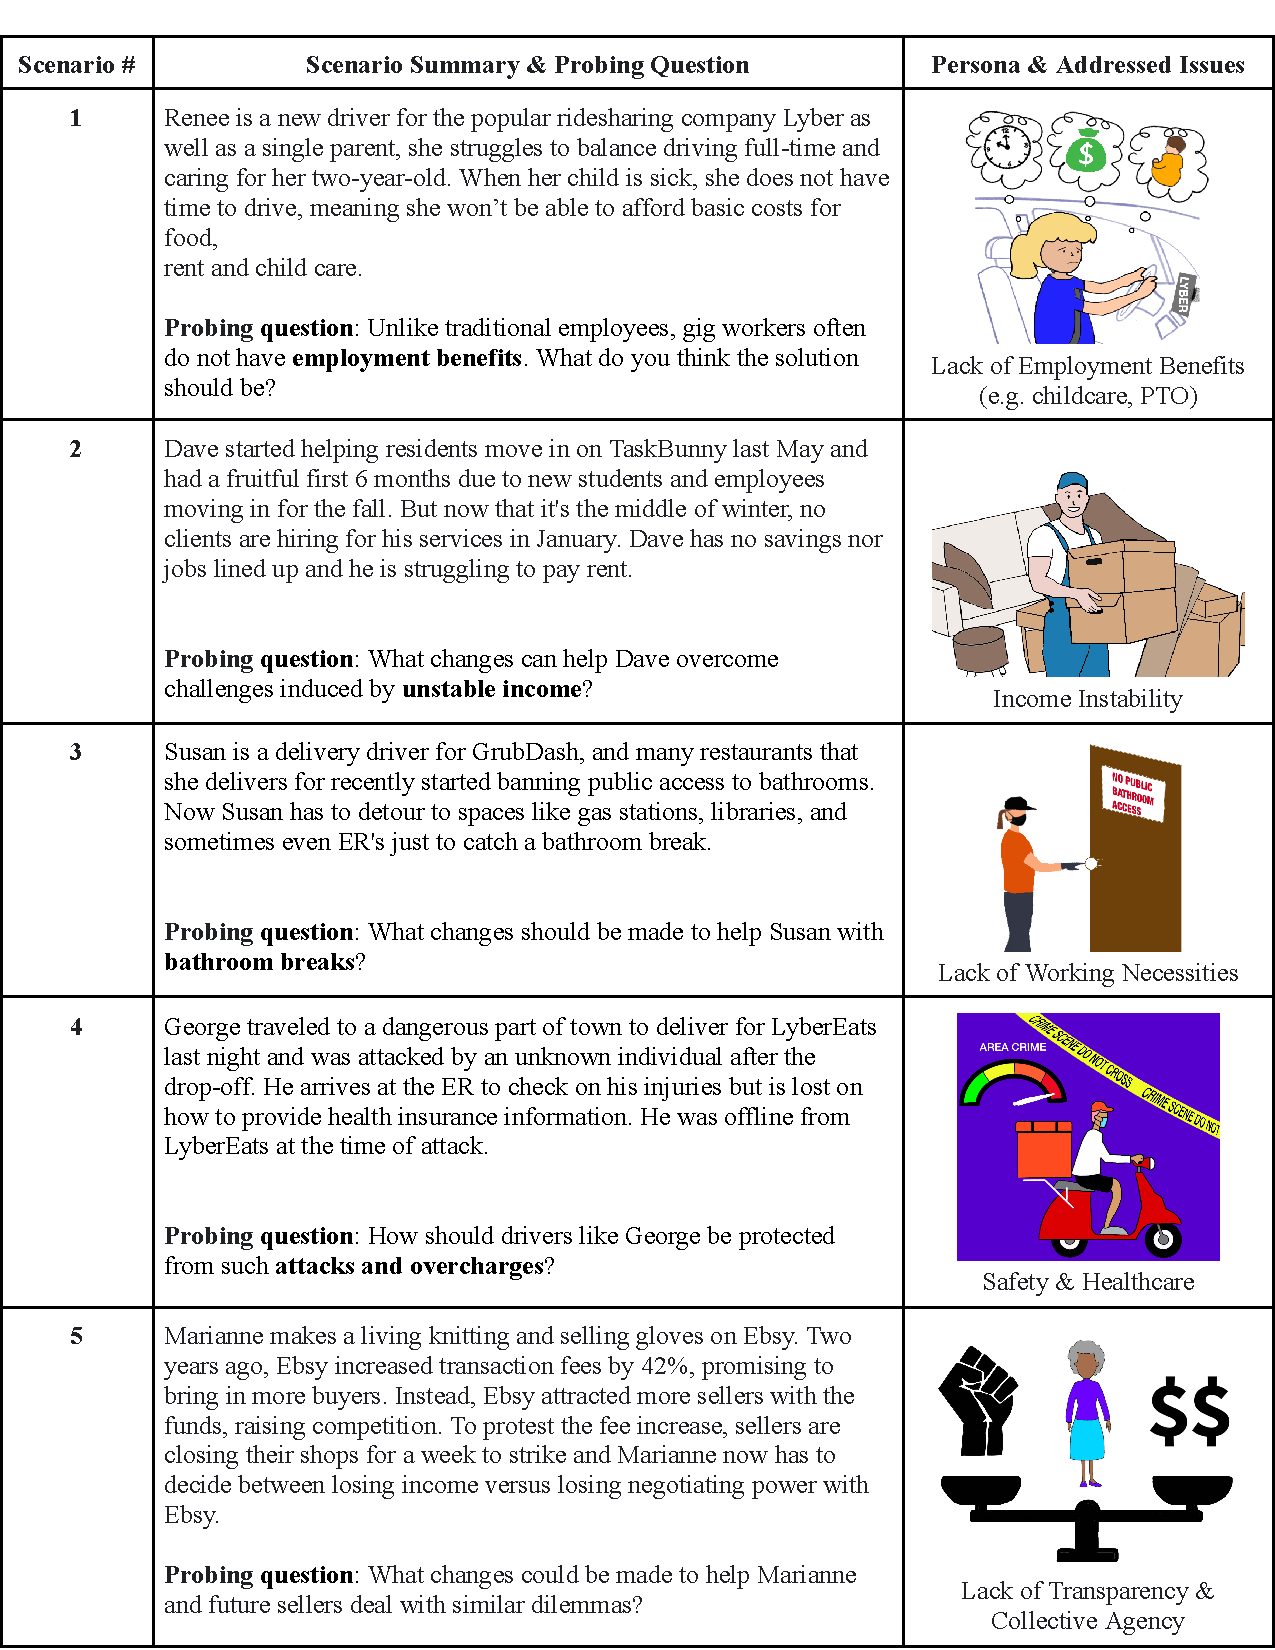
\includegraphics[width=\textwidth]{Chapters/ch4/scenarios.pdf}
  \label{tab:scenarios}
\end{table}
\FloatBarrier

\paragraph{Storyboards} To present these scenarios, we constructed five pictorial storyboards depicting stories based on news articles, local workshops, and prior work. Storyboarding, defined as ``a short graphical depiction of a narrative'', is an effective tool for demonstrating 1.) impacts of technologies on human activity and 2.) effects of proposed (technological) interventions and solutions before implementation. Since we cover a wide range of gig worker types in this study (e.g. food couriers, rideshare drivers, movers and online sellers), storyboards allow participants to quickly engage with specific situations, connecting their own lived experiences when applicable. 
Following  Truong et. al.'s guidelines \cite{truong2006storyboarding} on best practices for storyboarding (concise background, intentional text, characters, graphics, passing of time, etc.), we drew empathy from our participants using personas of gig workers, included text to orient participants in the character's world, and only constructed three frames per scenario to succinctly convey each character's activities to avert bogging participants down with overt details.

\paragraph{Procedures}
Each scenario was presented via three storyboard cards, and we guided conversation using a probing question that focuses discussions around broader underlying issues. 
After introducing the scenario and probing question, we requested that participants read the prepopulated solutions and treat them as seed solutions for generating their own ideas, and subsequently \textbf{rank all the solutions for the scenario}. 
% Table \ref{tab:solutions} and \ref{tab:rankings} in the Appendix show the generated solutions and an example instance of the ranking process. 
During the ranking process, we solicited the rationales of participants' ranking decisions to probe at and uncover latent social boundaries and desiderata. Due to time constraints, we did not engage our participants in a formal consensus building processes (e.g. the Delphi method) during rankings. After solution ranking, we asked a set of followup questions to wrap up each scenario. The scenarios were presented in the same order across all workshop sessions, as shown in Table \ref{tab:scenarios}.

After completing the above, participants were asked to \textbf{rank the five scenarios} in terms of what they thought were most important to address, effectively performing needs-validation over the issues we presented. In summary, we asked participants of each workshop to complete the following set of tasks, in order: 
\begin{enumerate}
    \item {For each of the five scenarios:}
    \begin{enumerate}
        \item {Examine the scenario's storyboard and accompanying descriptive text (including the probing question)}
        % \item {Optionally debrief the scenario with any questions, thoughts or ideas}
        \item Read through and discuss the list of prepared solutions, then add newly generated ideas
        \item {Rank the solutions (including the ideas generated live) based on preferences and priorities, using sticky notes}
        \item {Explain reasoning for ranking preferences}
        \item {List the most and least preferred solutions}
        \item {Express who should be responsible for implementing the mentioned solutions (using provided check-boxes)}
    \end{enumerate}
    \item {Rank the five scenarios in terms of which issues are most important to address}
\end{enumerate}
Participants were encouraged to add solutions at any point in these steps. Additional materials used for workshops are included in supplementary materials, and solutions generated by participants are available in the Appendix. 

\subsection{Workshop Setup}
We conducted a total of 8 co-design workshops with 20 participants, one of which was in-person while the rest were virtually conducted via Zoom. All participants were located in the United States and compensated at a rate of \$60/hour for their time, and each workshop lasted 90-120 minutes. To encourage discussion and collaboration among participants of the same stakeholder group, we included 2-3 participants in most workshops instead of conducting individual sessions. 
Combining the gig workers with the policymakers or platform employees could have discouraged workers to speak up in workshops, and thus we only included one stakeholder group in each workshop (Table \ref{tab:participants} indicates the relevant stakeholder group to each workshop). This separation was intended to avoid further disempowerment of already marginalized voices, and to minimize the emergence of power differentials that could have resulted from potential employment relationships  -- workers in one group may have been demotivated to express their honest opinions if the workshop also hosted their employer.
Because we studied our stakeholder groups separately, participants were able to connect and collaborate easily with peers from similar backgrounds. This setup of groups with similar experiences and values made each co-design workshop a productive discussion rather than confrontational. We also helped different participant groups collaborate asynchronously with each other by updating them on relevant solutions and rankings from previous workshop sessions.

Prior to each workshop, we set up whiteboards on Miro or physical easel pads to present the scenarios and potential solutions to participants, which served as a space for participants to rank or add solutions via sticky notes, and to document their finalized preferences. We took video recordings and field notes across workshops and collected participants' solution rankings, votes on who should take responsibility, and newly generated solutions.


\subsection{Positionality}

As Irani states, reflexivity in HCI allows us as researchers to produce better knowledge by ``recognizing designers' positions, values, limitations, and standpoints''. In the following, we reflect on our own positions as designers and researchers as well as how it impacts our work outputs \cite{irani2016stories}. We are all researchers residing in the US who work or receive training in the fields of Computer Science, Human Computer Interaction, and Music. Two of us live in the city where the study was conducted and have prior experience conducting research surrounding gig work. However, we recognize the relative privileges we hold in society as compared to worker participants. For instance, none of us have completed gig work ourselves and therefore lack first-hand experience of the issues that gig workers face. Additionally, we have all been a consumer on gig platforms; three authors often speak to rideshare workers about their job during rides and one author has family members who engage in gig work. The funding for this research sources solely from the National Science Foundation, and the work is not sponsored by any external companies or platforms.

We as researchers all hold the view that the current state of the gig economy, as discussed in Section 2, is incapable of supporting the well-being of gig workers and that these challenges should be addressed soon since it seems that gig work is here to stay. To address the need for change, we employ a combination of transformative, postmodern and pragmatic frameworks to interpret and understand the present day conditions of gig work, as well as to find practical approaches toward addressing some of these real world issues. \cite{Creswell2016-rq}. We presented day-to-day scenarios of individuals, which inform design decisions for addressing issues of gig work, and allows participants to generate solutions. In addition, we pre-populated the solution space with provocative ideas so as to give participants space for imagining more systematic solutions, which can contribute toward long-term reform of the gig-economy. 
%may bias our perspectives away from more systemic and collective changes. 
%We believe that this focus on present day scenarios will result in  However, this comes at the trade-off of not prompting participants towards  which we believe are essential for the 

Following best practices suggested by prior literature \cite{reinharz1992feminist, calvin, liang2021embracing}, we shared our affiliations and intentions with participants prior to workshops, reflected on our own biases as researchers, and pondered ``how can participants benefit from the study beyond the monetary compensation?'', ``are we bringing positive impacts to the worker community?'' and ``how can we place workers' ideas in a larger field of power?''.
We also include in \ref{limits} participant reflections on our study and considerations for future lines of research.

\subsection{Analysis}
To begin analysis, we first computed average rankings for each solution and extracted the three highest and lowest ranked solutions for each scenario based on these averages. We then engaged in a thematic analysis approach to analyze 14 hours of Zoom recordings (transcribed by the online service \textit{Rev.com}) and 18 pages of field notes. In the first stage of the analysis, we followed an opening coding approach, where one to two researchers independently conducted qualitative coding for each workshop's data (at least one of these coders was present at the corresponding workshop) \cite{Patton2014-ef, mcdonald2019reliability, Patton2014-ef, corbin2014basics, strauss1990basics}. During this process, coders remained receptive and looked for as many codes as possible, while keeping in mind our research questions on worker well-being, the issues that each scenario targets, and potential future changes. The coders met to refine and resolve any disagreements about the initial codes, resulting in a total of 567 unique codes. In the next stage of analysis, we iteratively combined these codes into emergent themes and subthemes, wrote descriptive memos, and built an affinity diagram to map the relationships between categories \cite{holtzblatt2014contextual, Beyer1999-hr}. This analysis produced 8 themes and 63 subthemes, and we describe these findings below. The first set of findings
gives an overview of participants' rationales for rankings across scenarios, the second set reports on scenario-based themes from participant's reactions and perspectives on our proposed solutions, and the last set describes themes from participant-generated solutions.

\FloatBarrier
\begin{table}[h!]
\centering
\caption{Summary of Stakeholder's Motivations and Deterrents}
 \label{tab:stakeholders}
 \resizebox{\textwidth}{!} {
\begin{tabular}{|l|l|l|}
\hline
\textbf{Stakeholders} & \textbf{Motivating factors and preferences} & \textbf{Deterrents} \\ \hline
Platform & \begin{tabular}[c]{@{}p{6.5cm}@{}} $\bullet$ Minimize worker decommission\\  $\bullet$ Required compliance to mandates and regulations \\  $\bullet$ Preserve public image\end{tabular} & \begin{tabular}[c]{@{}p{6cm}@{}}$\bullet$ Increased operation costs\\ $\bullet$ Thin profit margins \& market competition \\$\bullet$ Legal liabilities\end{tabular} \\ \hline
Workers & \begin{tabular}[c]{@{}l@{}}$\bullet$ Leverage multiple platforms\\ $\bullet$ Personalized solutions\end{tabular} & \begin{tabular}[c]{@{}p{6cm}@{}} $\bullet$ Disruptors to earning opportunities or client relations\\ $\bullet$ Short-term or unreliable solutions\end{tabular} \\ \hline
Regulators & \begin{tabular}[c]{@{}p{6.5cm}@{}}$\bullet$ Worker-initiated collective action\\  $\bullet$ Hold platforms responsible for initiating and implementing solutions that benefit their workers\end{tabular} & \begin{tabular}[c]{@{}p{6cm}@{}}$\bullet$ Providing special accommodations to specific worker subgroups \\ $\bullet$ Invasive monitoring of workers\end{tabular} \\ \hline
\end{tabular}
}
\end{table}
\FloatBarrier

\section{Results}
Each stakeholder group offered unique reactions to our scenarios and proposed solutions. Thus, we start by presenting overarching incentives and preferences that motivates each stakeholder group to initiate change, as well as factors that prevent them from implementing suggested solutions. Next we delve into individual scenarios to unfold participants' quantitative rankings of solutions and provide a debrief of their rationales using qualitative results. We end by describing participants' imagined solutions that spanned across workshops and scenarios.

\subsection{Multi-Stakeholders' Incentives, Preferences \& Deterrents}

In this section, we present themes that emerged across various scenarios, reporting on stakeholders' overall incentives and preferences that motivate them to promote change for improving gig worker well-being, as well as factors that deter them from implementing suggested solutions. These patterns were revealed through discussions during solution-ranking/generation; Table \ref{tab:stakeholders} summarizes these findings. 

\subsubsection{Platform Motivations \& Preferences}
\paragraph{Minimize Worker Decommission}
Platforms are inherently incentivized to support participating workers, since their operations depend critically upon labor supply. 
% When circumstances allow for platforms to provide assistance/benefits to workers, positive outcomes ensue for both groups. 
For example, when workers are decommissioned, platforms are motivated to bring them back on a job because ``if the worker's not making money, if the worker's not available to work or just isn't working, the platform is not making money'' (P1). 
Worker decommission can result from a variety of factors, including fluctuating seasonal demands, a lack of opportunities or unmet childcare needs: ``If somebody doesn't have childcare, that does make them less likely to be available for work on the platform, which is problematic for the platform'' (P1). 

\paragraph{Government Mandates and Regulations}
Regulatory pressure can incentivize platforms to make changes, but an excess of mandates can cause them to ``think that a lot of this regulation stifles innovation'' (P1). Mandates are also undesirable to platforms because since they mean ``that we're more restricted, that we're gonna have to pay more'' (P1). In addition to restricting platforms from implementing novel features, the cost of (unfunded) mandates can also ``significantly restrict our bottom line and our ability to continue to function as a platform'' (P1).

\paragraph{Preserving Public Image}
To circumvent additional regulations, platforms are willing to implement services to preserve public image and ``appease the general public or regulators or media \dots by offering something like a childcare program'' (P1). Platforms' aversion to regulation is strong enough to dedicate ``large government relation teams that \dots strongly lobby against'' mandates ``except where they think that it benefits them to show the public for PR reasons'' (P1).

\subsubsection{Deterrents for Platforms}
\paragraph{High Operation Costs}
Many of the solutions we presented called for the development of services or programs to benefit workers. Platforms cited high costs and other service priorities as reasons against implementation:  ``if we're adding incremental benefits, we have to reduce something else'' (P1). According to a P1 participant,  implementing a single feature can cost ``easily six months of three engineers time, plus maybe a month of design effort, plus \dots you're probably talking about an initiative it's gonna cost \$650,000'', and such initiatives may be so ``prohibitively expensive, to the degree [that] the platform might not continue to be sustainable''.

\paragraph{Thin Profit Margins}
One might suggest that platforms use resources gleaned from profit margins to develop features that promote worker well-being. However, platform-side participants relates how ``margins are getting tougher and tougher on a lot of these products and services'' (P1). In order to provide for increased pay or benefits, ``the platform effectively needs to take less'', but ``the company's not really gonna take less cut because [then] they couldn't pay their employees and they just have to cut heads'' (P1). Alternatively, platforms can ``increase price [of its service]'', but that instigates a negative cycle by putting the platform at risk for user abandonment because if ``you raise it too high, you lose customers automatically, they don't wanna pay 50 bucks to go five miles'', so it ``reduces the number of users that will use the platform, which will cause Lyber to make less'' (P1).

\paragraph{Competition Between Platforms}
Exacerbating monetary constraints, customers were deemed ``very price sensitive, they're fickle, they may open both [apps]'' (P1). If they are not satisfied with prices, clients might just abandon the service altogether: ``There is a maximum amount of money that Lyber passengers are willing to pay for a single trip where [they] start to see declines in usage'' (P1). In fact, platforms assign ``an entire revenue optimization team that figures out how much can be charged and how much people are willing to pay.'' (P1).


\paragraph{Legal Liabilities} 
In addition to costs, another factor that demotivates platforms from service offerings is their potential legal ramifications. Platform participants fear such potential complications and ``hope that there wouldn't be reputational risk to Lyber by Renee's[/workers'] kid[s], potentially getting injured by being taken care of by another parent'' (P1). Regulator participants also recognized the risks, noting that ``one of the reasons why childcare programs aren't on sites in corporations is [because] the liability is huge'' (R2). 
The ambiguous legal classification of gig workers also disincentives additional provisions of benefits since ``the more that you \dots treat somebody as if they're an employee, the more they can argue in court that they are an employee'' (P1). 

% One participants' employer platform had ``run into some pretty hairy legal issues around providing any type of benefits to our [workers] because they can't have anything that would make them legally deemed employees of [platform name] rather than contractors'' (P2).

\subsubsection{Worker Practices, Motivations \& Preferences}
\paragraph{Leverage Multiple Platforms} \label{multiapp}
To address instability, workers related experiences of engaging with multiple platforms at once: ``if things slow down on one platform, then you can go to another'' (W2). Distributing worker profiles across multiple platforms raises opportunities of procuring gigs, and workers view the labor of finding work as their own responsibility: ``you can't just sit there and say that TaskBunny should be responsible \dots when it's off season, it's upon you now to maybe seek other alternatives of earning'' (W1).
% To address instability, workers related experiences of engaging with multiple platforms at once: ``if things slow down on one platform, then you can go to another'' (W2). Distributing worker profiles across multiple platforms raises opportunities of procuring gigs, and workers view the task of finding work as their own responsibility: ``you can't just sit there and say that TaskBunny should be responsible \dots when it's off season, it's upon you now to maybe seek other alternatives of earning'' (W1).

\paragraph{Personalized Solutions} \label{personalized}
The instability of gigs often forces workers to fit needs around work schedules, but ironically the promised flexibility is oftentimes what drove them toward gigs in the first place \cite{lee2015working}. Thus it's on platforms to adjust around worker schedules, ``to understand the kind of situation that you're in and then they'll try to adjust to fit your availability \dots this is the best way \dots [when] they're trying to adjust to your schedule \dots [and] to your situation'' (W1). Adjusting to workers' circumstances can provide a peace of mind through both regularity on standard days and accommodations during emergencies. Platforms don't currently account for situations where ``[there is an] employee who is on maternity leave \dots [or] away for stuff like funerals'', but workers desire solutions that consider ``the various kinds of condition[s] that needs them to be away from work'' (W1).

\subsubsection{Deterrents for Workers}
\paragraph{Impediments to Earning or Damages to Client Relations}
Worker participants held a strong aversion against changes that conflict with their own priorities (e.g. making earnings, maintaining good reputation with clients). For example, when presented with Susan's predicament of being blocked from restaurant bathrooms, one worker explained how ``you need to work to get money'', challenging the hypothetical idea that if ``all the restaurants fail to offer bathroom services, do you stop working?'' (W1). Another worker opposed ``the restriction of platforms, [since] that means you wouldn't have work'' (W2). They were also mindful of client relationships, stating concerns that ``avoid[ing] orders from those locations, meaning that the clients would suffer'' (W2)% and ``people living in [those] particular area[s] need their deliveries on time'' (W1)
. Beyond clients, workers also ``wouldn't want to get on a restaurant's bad side'' (W2).


% . For example, they consistently oppose solutions that hinder their objective of making earnings, including those that harm their relations with clients. 

\paragraph{Short-term or Unreliable Solutions}
Temporary solutions were also undesirable to workers, as they offer only short-lived relief to long-lasting problems. While some help is better than nothing, ``they are just short term, they may be a day or two solutions in a month, in the whole season'' (W2). For childcare needs, ``[days of paid time off] is not a solution because \dots she has to stay with the kid'' (W1). Worker participants also resisted solutions out of their control, since they may be breakable -- ``security equipment could fail, maybe the cameras have failed to work, or failed to capture a clear image of the attack'' (W1) -- or unreliable -- ``off-season events that are planned by TaskBunny maybe would not be very reliable'' (W2).

\subsubsection{Regulator Motivations \& Preferences}
\paragraph{Hold Platforms Accountable}
Regulator participants held companies largely responsible to creating better working conditions for their employees. One R3 participant emphasizes how ``it's the company's responsibility to create a work environment that is conducive to people succeeding and building the lives that they want''. Specifically, they ``could imagine a world in which the platform invests in safe bathroom facilities for their own people'' (R3). In addition to bathroom access, one regulator also contended that ``platforms are viable for healthcare consequences associated with the work that their people are doing'' (R3).

\paragraph{Worker-initiated Collective Efforts} \label{worker_action}
Power and informational asymmetries makes regulators ``reluctant to say the burden should fall on one person's shoulder to save themselves'' (R3). Instead, regulator participants recommended ``finding ways for the gig workers to combine effectively'' (R3), through collective worker actions such as pooling, unionizing and striking to impose pressure on platforms to initiate change. 
But since gig workers are not employees, many questions exist around how to collectively organize and bargain: ``How do you strike when you're not a union? How do you strike and what do you demand?'' (R2). 
Soliciting company involvement was one potential solution: ``If not in a formal union, having a company that gives their employees the opportunity to convene and to say what matters most to them could be good as a company practice or policy'' (R2).

\subsubsection{Deterrents for Regulators}
\paragraph{Special Accommodations for Particular Subgroups}
Regulators repeatedly emphasized inclusion (of workers and customers alike) and resisted special accommodations for specific groups. They raised additional questions like ``Do you have it for the single dad? Do you have it for like elder care? Where do you stop?'' (R3). 
For instance, while the idea of issuing badges to workers helps with limits on bathroom access, it also prompts problems of privacy and misuse: ``thing about badges \dots is that even if they're voluntary, any program of self-identification creates risks \dots with prospective privacy vulnerable populations, you can't really predict how that kind of information is going to circulate and be used in an inappropriate way'' (R3). 
In general, regulator participants objected to ``the idea of demarcating workers differently \dots that's dangerous and creates fault lines between people \dots even if \dots you're not closely tied to each other'' (R2). Thus, it's imperative ``for the company to have its own policies (designed either by mandate or by voluntary corporate structure) to be as inclusive [of] as many different types of workers as possible'' (R3). 

\paragraph{Violations of Worker Privacy}
Regulators also opposed invasive monitoring of workers, citing a violation of basic human rights. 
For example, ``a single mom badge come with risk \dots [you can imagine] some sketchy dude who likes to pick up women with kids and abuse them, then I think identifying someone as such could lead to safety concerns'' (R2). 
Another participant protests how ``we've gotten to the point where, because of technology and oversight, people have literally no independence - they can't even go to the bathroom on their own [initiative] anymore \dots [it's] kind of a human rights violation to have that kind of deep oversight of your employee'' (R3).
Monitoring via dash cams also pose issues of invasion, for while they allow workers ``to share [footage]\dots with the police so that they can help solve the crime'', they may also be ``pointing in at them as they're driving, I could see just a huge amount of privacy concerns rising from that'' (R3). 


\subsection{Scenario Rankings and Rationales}
In the following scenario-based analysis, we include the top three most favored solutions as well as disliked solutions, and indicate the workshops that casted their votes via a bracked list of workshop IDs. Some solutions triggered polarizing opinions across different stakeholder groups, and may therefore simultaneously appear as both favored and disliked. To elucidate the strength of preference, we include the average rankings of individual solutions across all workshops, where lower rankings indicate more preferred solutions. To summarize each scenario, we wrap up with a recap of tensions between stakeholder groups and acceptable solutions that are common grounds to multiple stakeholder groups. 

\FloatBarrier
\begin{table*}[h]
\centering
\caption{Scenario 1 Rankings and Voting Summary}
\label{tab:s1}
\resizebox{\textwidth}{!} {
\begin{tabular}{|l|llc|}
\hline
\multirow{8}{*}{\begin{tabular}[c]{@{}c@{}}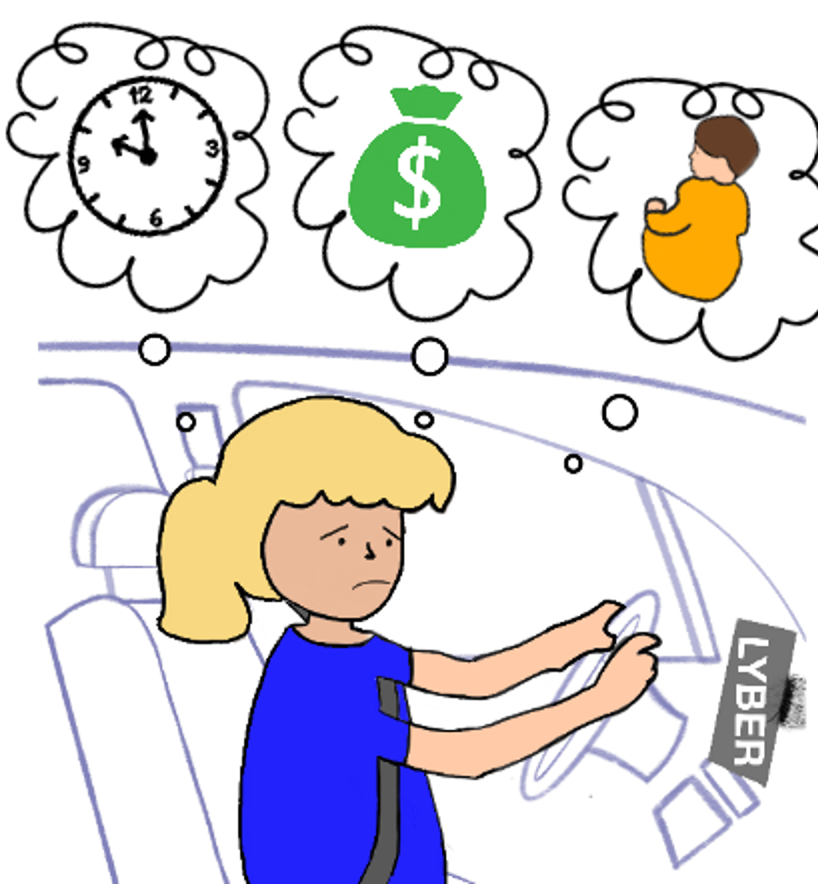
\includegraphics[width=2.75cm]{Chapters/images/renee.png} \\ {Renee balancing} \\ {rideshare work} \\ {and childcare.}\end{tabular}} & \multicolumn{2}{c|}{\textbf{Scenario 1} {(Absence of employment benefits)}}                                &  \begin{tabular}[c]{@{}c@{}}\textbf{Avg Ranking} \\ (lower = preferred)\end{tabular} \\ \cline{2-4} 
                  & \multicolumn{1}{l|}{\multirow{3}{*}{\begin{tabular}[c]{@{}c@{}}Top 3 \\ most \textbf{favored}\\  solutions\end{tabular} }} & \multicolumn{1}{l|}{{Platform offers childcare program {[}R1-2, W1-2, P3{]}}} & 2.625 \\ \cline{3-4} 
                  & \multicolumn{1}{l|}{}                  & \multicolumn{1}{l|}{Paid Time Off (PTO) {[}R1-3, W2{]}} & 3.313 \\ \cline{3-4} 
                  & \multicolumn{1}{l|}{}                  & \multicolumn{1}{l|}{Driver-support groups {[}R3, W1, P1{]}} &  3.313 \\ \cline{2-4} 
                  & \multicolumn{1}{l|}{\multirow{3}{*}{\begin{tabular}[c]{@{}c@{}}Top 3 \\ most \textbf{disliked}\\   solutions\end{tabular}}} & \multicolumn{1}{l|}{Platform offers higher hourly pay {[}R1, W1-2, P1-2{]}} & 5.250 \\ \cline{3-4} 
                  & \multicolumn{1}{l|}{}                  & \multicolumn{1}{l|}{\begin{tabular}[l]{@{}l@{}}Worker adds incentives to encourage tips \\ {[}R2-3, W1{]}\end{tabular}} & 4.625 \\ \cline{3-4} 
                  & \multicolumn{1}{l|}{}                  & \multicolumn{1}{l|}{\begin{tabular}[l]{@{}l@{}}Knowing the destination of incoming rides \\ {[}R1, R3, W1, P2{]}\end{tabular}}  & 4.688 \\ \cline{2-4} 
                  & \multicolumn{1}{l|}{\begin{tabular}[c]{@{}c@{}}Who should be \\ responsible for \\ making changes\end{tabular} }                  & \multicolumn{2}{l|}{\begin{tabular}[c]{@{}l@{}}$\bullet$ 7 of 8 workshops voted platforms [R1, R2, R3, W1, W2, P2, P3] \\ $\bullet$ 4 of 8 workshops voted workers [W1, W2, P1, P2] \\ $\bullet$ 5 of 8 workshops voted regulators [R1, R2, R3, P2, P3] \end{tabular}}    \\ \hline
\end{tabular}
}
\end{table*}
\FloatBarrier

\paragraph{Scenario 1 -- Absence of Employment Benefits (e.g. childcare, PTO)} \label{s1}

Worker and regulator participants preferred benefits such as childcare or part time off, which most workshops decided it was on platforms to implement. 
Platform-initiated development of childcare programs was considered especially ideal since it offers more flexibility in implementation, but the fear of receiving mandates does drive platforms towards action. In addition to childcare, paid time off can similarly offer temporary relief to Renee's situation. However, platforms were reluctant to provide benefits like these due to restricted funding. As non-employees, workers are currently not guaranteed allowances like paid time off or childcare support, and platforms fear that any government mandates requiring so might incur additional costs.
As an exception, regulators from Washington state have set an example for other localities by granting gig workers certain guarantees like sick leave or minimum wage, without sacrificing their status as an independent contractor\footnote{Bill HB2076 offers Washington drivers sick leave and minimum wage standards when they transport a passenger in their car: \url{https://lawfilesext.leg.wa.gov/biennium/2021-22/Pdf/Bills/House\%20Passed\%20Legislature/2076-S.PL.pdf?q=20220309063519}}. Finally, regulators and platforms were both inclined to avoid regulatory micromanagement, but welcome platform-initiated changes, which could be incentivized by regulations. One way to motivate rather than regulate platforms is through taxation mechanisms, where platforms either receive a tax break for providing a certain benefit, or pay the a tax for the government to provide the benefit to workers. Some platform designers may prefer this solution since a worker benefit program or service with regulation might mandate a specific timeline or a particular way of implementation.

\textbf{Summary of stakeholder stances and recommendations}: All valued worker benefits (e.g., childcare and PTO) highly, and were inclined to think that platforms implement and pay for it. But platforms were reluctant to act due to associated costs and legal liabilities. Regulators can incentivize platforms by mandating some workers benefits, but should guard against micromanaging the execution of such initiatives.

% \FloatBarrier
\begin{table*}[h!]
\centering
\caption{Scenario 2 Rankings and Voting Summary}
 \label{tab:s2}
\resizebox{\textwidth}{!} {
\begin{tabular}{|l|llc|}
\hline
\multirow{8}{*}{\begin{tabular}[c]{@{}c@{}}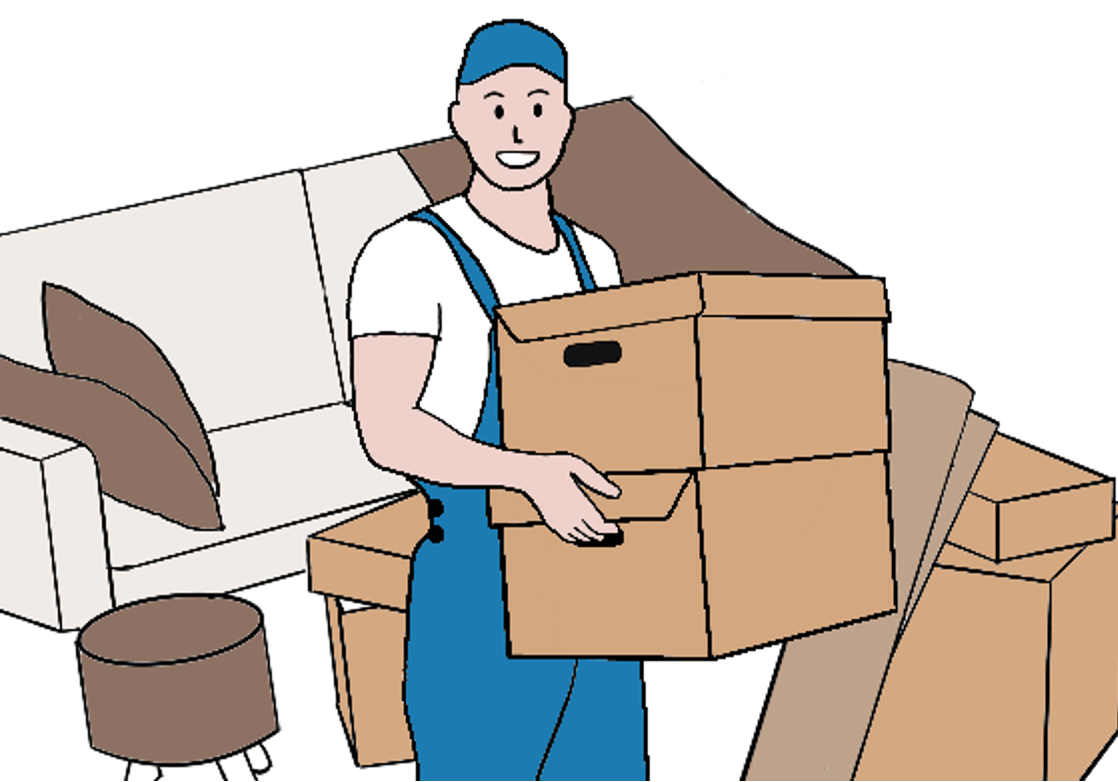
\includegraphics[width=2.75cm]{Chapters/images/dave.png} \\ {Dave facing}\\ {seasonal lows in} \\ {job opportunities.}\end{tabular}} & \multicolumn{2}{c|}{\textbf{Scenario 2} {(Income instability)}}                                & \textbf{Ranking} \\ \cline{2-4} 
& \multicolumn{1}{l|}{\multirow{3}{*}{\begin{tabular}[c]{@{}c@{}}Top 3 \\ most \textbf{favored}\\  solutions\end{tabular} }} & \multicolumn{1}{l|}{Winter side hustles/off-season work recommendation {[}all{]}} & 1.000 \\ \cline{3-4} 
& \multicolumn{1}{l|}{}                  & \multicolumn{1}{l|}{Platforms plan events during off seasons {[}R2, P1, P3{]}} & 3.875 \\ \cline{3-4} 
& \multicolumn{1}{l|}{}                  & \multicolumn{1}{l|}{Workers conduct long-term financial planning {[}W1-2{]}} & 4.188 \\  \cline{2-4} 
& \multicolumn{1}{l|}{\multirow{3}{*}{\begin{tabular}[c]{@{}c@{}}Top 3 \\ most \textbf{disliked}\\   solutions\end{tabular}}} & \multicolumn{1}{l|}{Workers conduct long-term financial planning {[}R1-2, P1-2{]}} & 4.188 \\ \cline{3-4} 
& \multicolumn{1}{l|}{}                  & \multicolumn{1}{l|}{Platforms plan events during off seasons {[}R3, W1-2, P2{]}} & 3.875 \\ \cline{3-4} 
& \multicolumn{1}{l|}{}                  & \multicolumn{1}{l|}{Regulators provide unemployment benefits {[}R2, P1{]}} & 4.188 \\ \cline{2-4} 
& \multicolumn{1}{l|}{\begin{tabular}[c]{@{}c@{}}Who should be \\ responsible for \\ making changes\end{tabular} }                  & \multicolumn{2}{l|}{\begin{tabular}[c]{@{}l@{}}$\bullet$ 8 of 8 workshops voted platforms [R1, R2, R3, W1, W2, P1, P2, P3] \\ $\bullet$ 5 of 8 workshops voted workers [R1, W1, W2, P1, P3]\\ $\bullet$ 3 of 8 workshops voted regulators [R2, W2, P2]\end{tabular}}    \\ \hline
\end{tabular}
}
 
  % \vspace{-8mm}
\end{table*}
\FloatBarrier

\paragraph{Scenario 2 -- Income Instability} \label{s2}
Platforms are overwhelmingly happy to plan off-season events to help decommissioned workers, since it also brings them earnings. In fact, one participant's employer platform already offers an effective incentive program for workers to complete snow removal jobs. One way of encouraging client engagement that participants recommended was the initiation of a ``spring-cleaning week'', which would prompt them toward a task that they wouldn't otherwise think about. Such events advantage workers by giving them information that substitutes for the social network they would've relied on informally. However, workers worry that income from platform-initiated events offer only minor gains, not long-term solutions -- it was imperative to workers that they can plan for and control their own financial situations. One way that workers can curb the effects of seasonal fluctuations was to leverage the availability of multiple platforms, so that when they don't have work at TaskBunny, they can earn through jobs somewhere else. Platforms can also help workers conduct financial planning by including features like in-app earnings projections. Finally, platforms are disinclined to provide unemployment benefits, citing (on top of costs) how disbursing unemployment funds upfront may cause recipients to immediately spend it or lose their motivation to work.


% In fact, one participant's company has already begun ``offer[ing] an incentive to [workers] \dots whenever there's a snowstorm \dots to complete a certain amount of snow removal jobs. And if they do that, they get an incentive payout \dots it definitely was deemed effective by ops and there was a large majority of [workers who] were paid out'' (P2). 
% for this incentive and a lot of people that typically wouldn't have ever done snow removal. We saw a huge bump in registration in those categories. So that seems to be pretty effective


% Instead, the participant suggested that since a major platform is usually ``a company with much cash flow, it's not a huge deal to advance an extremely trustworthy partner, \$1,500 or something like that to help them get through'', serving as ``discretionary funds that are available for specifically emergency situations''.

\textbf{Summary of stakeholder stances and recommendations}: Compared to platform-planned off-season events, workers preferred to be in control of their own financial planning. Since platforms were unwilling to provide unemployment benefits, workers can overcome seasonal lows by engaging with alternative platforms. Such worker inclinations toward increased agency presents unique opportunities for HCI designers to invent technological solutions for workers that integrate multiple platforms and facilitate cross-platform information sharing.

% \FloatBarrier
\begin{table*}[h!]
\centering
\caption{Scenario 3 Rankings and Voting Summary}
\label{tab:s3}
\resizebox{\textwidth}{!} {
\begin{tabular}{|l|llc|}
\hline
\multirow{8}{*}{\begin{tabular}[c]{@{}c@{}}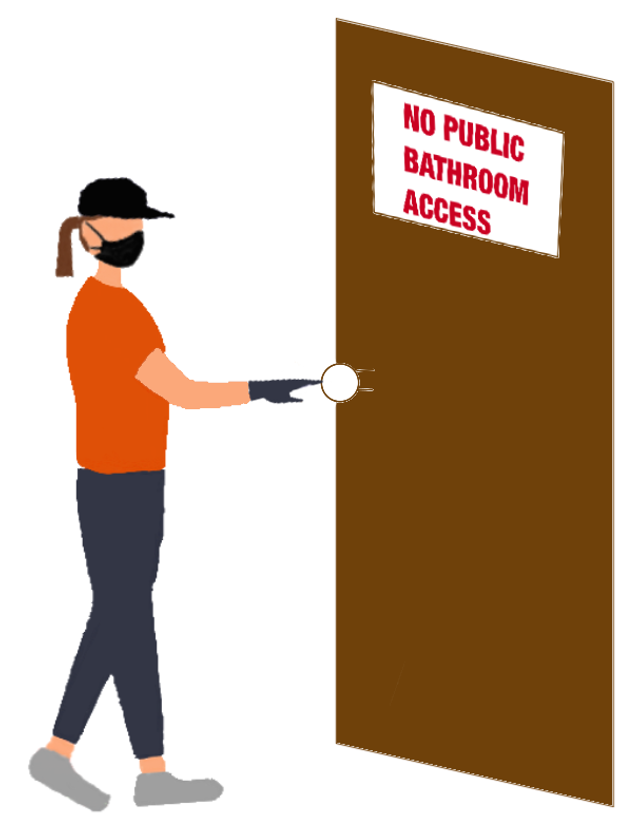
\includegraphics[width=1.5cm]{Chapters/images/susan.png} \\ {Susan struggling}\\ {to access bathrooms} \\ {at restaurants that} \\ {she delivered for.}\end{tabular}} & \multicolumn{2}{c|}{\textbf{Scenario 3} {(Missing Access to Working Necessities)}}                                & \textbf{Ranking} \\ \cline{2-4} 
& \multicolumn{1}{l|}{\multirow{3}{*}{\begin{tabular}[l]{@{}c@{}}Top 3 \\ most \textbf{favored}\\  solutions\end{tabular} }} & \multicolumn{1}{l|}{\begin{tabular}[l]{@{}l@{}}Platforms negotiate with restaurants \\ to open bathroom locations to workers. {[}R1, W1-2, P2-3{]}\end{tabular} } & 2.188 \\ \cline{3-4} 
& \multicolumn{1}{l|}{}                  & \multicolumn{1}{l|}{\begin{tabular}[l]{@{}l@{}}
Platforms show public bathroom locations in apps. \\ {[}R1, P1-3{]} \end{tabular}} & 2.125 \\ \cline{3-4} 
& \multicolumn{1}{l|}{}                  & \multicolumn{1}{l|}{\begin{tabular}[l]{@{}l@{}}Regulators require restaurants to provide bathroom access. \\ {[}R1-2, W1-2{]}\end{tabular}} & 4.188 \\  \cline{2-4} 
& \multicolumn{1}{l|}{\multirow{3}{*}{\begin{tabular}[c]{@{}c@{}}Top 3 \\ most \textbf{disliked}\\   solutions\end{tabular}}} & \multicolumn{1}{l|}{\begin{tabular}[l]{@{}l@{}}
Platforms cut off online orders during busy hours. \\ {[}R1-3, W1, P1-3{]}
\end{tabular}} & 7.688 \\ \cline{3-4} 
& \multicolumn{1}{l|}{}                  & \multicolumn{1}{l|}{Workers petition restaurants for bathroom access. {[}R2, P2{]}} & 5.375 \\ \cline{3-4} 
& \multicolumn{1}{l|}{}                  & \multicolumn{1}{l|}{\begin{tabular}[l]{@{}l@{}}
Workers share public bathroom locations with \\ one another.  {[}W1, P2{]}\end{tabular}}  & 5.188 \\ \cline{2-4} 
& \multicolumn{1}{l|}{\begin{tabular}[c]{@{}c@{}}Who should be \\ responsible for \\ making changes\end{tabular} }                  & \multicolumn{2}{l|}{\begin{tabular}[c]{@{}l@{}}$\bullet$ 8 of 8 workshops voted platforms [R1, R2, R3, W1, W2, P1, P2, P3]\\ $\bullet$ 3 of 8 workshops voted workers [W1, W2, P1]\\ $\bullet$ 7 of 8 workshops voted regulators [R1, R2, R3, W1, W2, P1, P2]\end{tabular}}    \\ \hline
\end{tabular}
} 
\end{table*}

\FloatBarrier

\paragraph{Scenario 3 -- Missing Access to Working Necessities} \label{s3}
All workshops recognized bathroom access as a basic need. As service-providers to restaurants, workers (along with regulators) felt adamant that deliverers like Susan should not be denied necessary access to bathrooms. One worker was willing to publicly voice such opinions through petitions and suggested that platforms issue badges to workers so that they can be given direct bathroom access in restaurants.
While regulator participants conceded that public infrastructure improvements are needed to build more clean and safe bathrooms, they also believe it is platforms' responsibilities to negotiate with restaurants, and to share with the workers a map indicating restaurants where the public is allowed to use the restroom. Unfortunately, platforms were reluctant to require bathroom access for workers from restaurants because they predict a drop-off in the number of participating restaurants. One platform participant commented that it's really hard to make  bathroom access mandatory from the food safety perspective. On the other hand, a regulator also noted how there are health code requirements that expect bathrooms to be publicly accessible. Bathrooms are one instance of underdeveloped public service, and in general we find that gig work exposes a lack of basic, fundamental safety nets in our public infrastructure.

\textbf{Summary of stakeholder stances and recommendations}: Our existing public infrastructure does not offer enough safe and public bathrooms, and gig work is starting to probe at the social boundary between platforms, restaurants, and workers regarding how workers should access facilities like bathrooms that are essential for work. Platforms can offer technological support by integrating restroom locations into maps and incorporating restroom breaks into route planning.

% \FloatBarrier
\begin{table}[h!]
\centering
\caption{Scenario 4 Rankings and Voting Summary}
\label{tab:s4}
\resizebox{\textwidth}{!} {
\begin{tabular}{|l|llc|}
\hline
\multirow{8}{*}{\begin{tabular}[c]{@{}c@{}}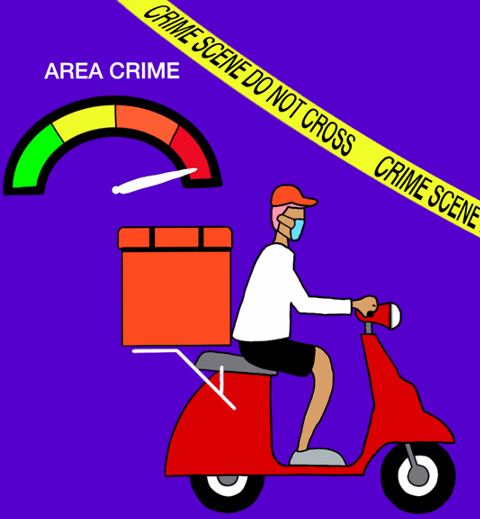
\includegraphics[width=2.75cm]{Chapters/images/george.png} \\ {George receives a high} \\ {medical bill for injuries} \\ {received from an attack at} \\ { an unsafe area after a delivery.}\end{tabular}} & \multicolumn{2}{c|}{\textbf{Scenario 4} {(Undermined Safety \& Worker Protections)}}                                & \textbf{Ranking} \\ \cline{2-4} 
& \multicolumn{1}{l|}{\multirow{3}{*}{\begin{tabular}[l]{@{}c@{}}Top 3 \\ most \textbf{favored}\\  solutions\end{tabular} }} & \multicolumn{1}{l|}{Regulators pass universal healthcare. {[}R2-3, W1-2, P2{]}} & 3.375 \\ \cline{3-4} 
& \multicolumn{1}{l|}{}                  & \multicolumn{1}{l|}{Platforms provide security equipment. {[}R1-2, W1, P3{]}} & 3.250 \\ \cline{3-4} 
& \multicolumn{1}{l|}{}                  & \multicolumn{1}{l|}{Platforms provide worker's compensation. {[}R1-2, W2, P2{]}} & 3.250 \\  \cline{2-4} 
& \multicolumn{1}{l|}{\multirow{3}{*}{\begin{tabular}[c]{@{}c@{}}Top 3 \\ most \textbf{disliked}\\   solutions\end{tabular}}} & \multicolumn{1}{l|}{\begin{tabular}[l]{@{}l@{}}
\begin{tabular}[l]{@{}l@{}}
Regulators restrict platforms from sending drivers to \\ high-crime areas.  {[}R2-3, W1-2, P1-3{]}
\end{tabular}
\end{tabular}} & 7.563 \\ \cline{3-4} 
& \multicolumn{1}{l|}{}                  & \multicolumn{1}{l|}{\begin{tabular}[l]{@{}l@{}}
Regulators require platforms to issue a warning \\ when workers enter high-crime areas. {[}R2-3, W1-2, P2{]} \end{tabular}} & 5.250 \\ \cline{3-4} 
& \multicolumn{1}{l|}{}                  & \multicolumn{1}{l|}{\begin{tabular}[l]{@{}l@{}}
Platforms provide workers additional subsidies  \\ for serving in high-crime areas. {[}R2-3{]}\end{tabular}} & 4.875 \\ \cline{2-4} 
& \multicolumn{1}{l|}{\begin{tabular}[c]{@{}c@{}}Who should be \\ responsible for \\ making changes\end{tabular} }                  & \multicolumn{2}{l|}{\begin{tabular}[c]{@{}l@{}}$\bullet$ 8 of 8 workshops voted platforms [R1, R2, R3, W1, W2, P1, P2, P3]\\ $\bullet$ 2 of 8 workshops voted workers [W1, P1]\\ $\bullet$ 6 of 8 workshops voted regulators [R1, R2, R3, W1, P2, P3]\end{tabular}}    \\ \hline
\end{tabular}
}
\end{table}
\FloatBarrier

\paragraph{Scenario 4 -- Undermined Safety \& Worker Protections} \label{s4}
The idea of restricting deliveries in high crime areas was rejected by all three stakeholder groups. In particular, regulators discouraged investing in technological improvements (e.g. signals and buttons and alerts) because identifying dangerous locations can evolve into digital redlining, thereby reinforcing existing stigma surrounding the place. Cutting off orders hurts restaurants because it generates less revenue, harms drivers by reducing their income, and angers hungry people since they can't get food delivery. Regulators recognized how this scenario calls attention to underlying issues of unsafe communities, and to address these, all workshops voted for platforms to contribute toward community safety improvements, through provisions of a safe operational vehicle, personal protective equipment etc. But security measures shouldn't really mean just the equipment, it also involves security personnel, which can take the form of visible public presences such as the police. Unfortunately, the public police force in general is overstretched and underfunded. Even if emergency buttons directing to the police were to be implemented, they would be fraught with issues related to fair distribution -- people would wonder why higher status law enforcement is more responsive to the platforms and its drivers, raising questions like ``Why did GrubHub drivers get the button? Why doesn't everybody get a button?'' (R3). Worker and regulator participants also thought that platforms should provide workers' compensation, especially if the injuries were received in area where workers arrived to for a gig. From a worker's perspective, those compensations could go a long way in helping George pay for his bills. Lastly, a regulator suggested providing more available medical facilities so that workers can have ``a place where they can go and get that quick healthcare'' (R2).

\textbf{Summary of stakeholder stances and recommendations}: Segregating areas by restricting (delivery) services in  high-crime locations is not the way forward. Regulators and platforms should work together to improve community safety. In particular, platforms should invest in security equipment for workers while regulators can provide more visible public presences as security personnel. 

\begin{table*}[h!]
\centering
\caption{Scenario 5 Rankings and Voting Summary}
\label{tab:s5}
\resizebox{\textwidth}{!} {
\begin{tabular}{|l|llc|}
\hline
\multirow{8}{*}{\begin{tabular}[c]{@{}c@{}}\\ 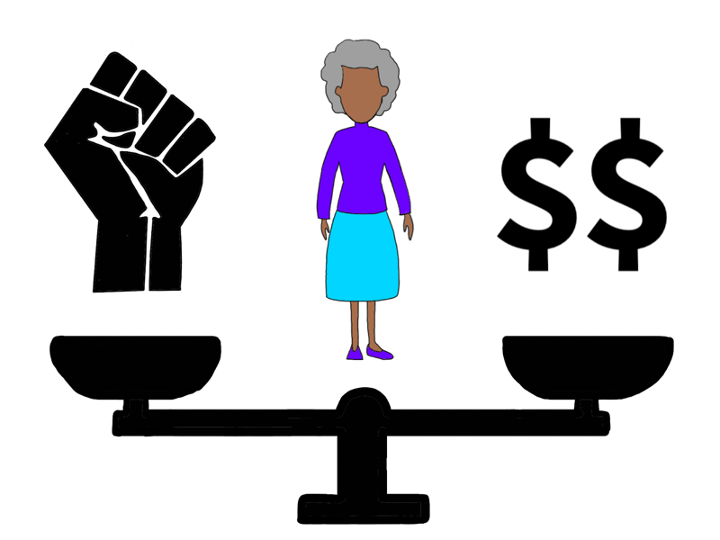
\includegraphics[width=2.75cm]{Chapters/images/marianne.png} \\ {Marianne's earnings} \\ {were compromised} \\ {after intransparent and} \\ {unfair platform decisions}\end{tabular}} & \multicolumn{2}{c|}{\textbf{Scenario 5} {(Intransparency \& need for collective action)}}                                & \textbf{Ranking} \\ \cline{2-4} 
& \multicolumn{1}{l|}{\multirow{3}{*}{\begin{tabular}[l]{@{}c@{}}Top 3 \\ most \textbf{favored}\\  solutions\end{tabular} }} & \multicolumn{1}{l|}{\begin{tabular}[l]{@{}l@{}}
Platforms implement transparent policies \\ about decisions to keep workers informed. {[}W1, P1, P3{]}
\end{tabular}} & 3.750 \\ \cline{3-4} 
& \multicolumn{1}{l|}{}                  & \multicolumn{1}{l|}{\begin{tabular}[l]{@{}l@{}}
Workers notify buyers of their situation \\ to garner support. {[}R1-R3{]}
\end{tabular}} & 3.875 \\ \cline{3-4} 
& \multicolumn{1}{l|}{}                  & \multicolumn{1}{l|}{\begin{tabular}[l]{@{}l@{}}
Regulators impose a ceiling on transaction fees. \\ {[}R1, R3, W1{]}
\end{tabular}} & 4.250 \\  \cline{2-4} 
& \multicolumn{1}{l|}{\multirow{3}{*}{\begin{tabular}[c]{@{}c@{}}Top 3 \\ most \textbf{disliked}\\   solutions\end{tabular}}} & \multicolumn{1}{l|}{\begin{tabular}[l]{@{}l@{}}
\begin{tabular}[l]{@{}l@{}}
Workers pool savings to strike without losing income. \\ {[}R1-2, P1-2{]}
\end{tabular}
\end{tabular}} & 6.000 \\ \cline{3-4} 
& \multicolumn{1}{l|}{}                  & \multicolumn{1}{l|}{\begin{tabular}[l]{@{}l@{}}
Workers maintain a good relationship with platform \\ by not participating in the strike {[}R2-3, P2{]} \end{tabular}} & 5.625 \\ \cline{3-4} 
& \multicolumn{1}{l|}{}                  & \multicolumn{1}{l|}{\begin{tabular}[l]{@{}l@{}}
Workers participate in the strike by stopping sales. \\ {[}W1, P1-2{]}\end{tabular}} & 4.313 \\ \cline{2-4} 
& \multicolumn{1}{l|}{\begin{tabular}[c]{@{}c@{}}Who should be \\ responsible for \\ making changes\end{tabular} }                  & \multicolumn{2}{l|}{\begin{tabular}[c]{@{}l@{}}$\bullet$ 6 of 8 workshops voted platforms [R2, W1, W2, P1, P2, P3]\\ $\bullet$ 5 of 8 workshops voted workers [R1, R3, W1, W2, P2]\\ $\bullet$ 5 of 8 workshops voted regulators [R2, R3, W1, W2, P3]\end{tabular}}    \\ \hline
\end{tabular}
}
\end{table*}

\FloatBarrier

\paragraph{Scenario 5 -- Intransparency \& need for collective action} \label{s5}

Transparent policies were most desired by both worker and platform participants, so that sellers like Marianne have time to plan for drastic changes. Because Ebsy failed to communicate their decisions to workers like Marianne ahead of time, now she has to deal with the dilemma of whether or not to strike. Even platform employees thought Ebsy ``definitely did a wrong thing'' by destroying their ``long-term trust situation'' with sellers through intransparency, which is ``something we should avoid, and the regulators should require transparent policies \dots because sellers is actually why your platform exist[s]'' (P1). To help workers achieve financial stability, platform participants recommended sellers strengthen their portfolio by putting their products on different platforms. This strategy of multi-apping is commonly employed even before the pandemic, and across continents \cite{goods2019your}. 
Regulator participants heavily encouraged workers like Marianne to participate in collective actions such as strikes, citing a list of reasons: it is a way of gaining power, Marianne owes her coworkers the support, and because solidarity is what makes strikes work. 
However, regulators also acknowledged the difficulties of collective organization, since it requires a ``certain savvy with regard to using social media'' (R3), which requires careful planning as a community. Indeed, workers strongly resisted engaging in collective action (as is observable through the most disliked solutions), expressing that they did not feel ``comfortable having their savings pooled together'' (W2). One platform participant also recommended that workers refrain from striking and ``maintain a good relationship with Ebsy'' (P1), rationalizing that doing so can advantage Marianne by boosting her sales while other sellers strike. 
% One participant who promoted multi-apping made an analogy to ``\textit{Who moved my cheese?} -- that book we read about pivoting in tough times'' (P2). 
% \add{Even p}\delete{P}latform employees \add{like P3} conceded 

\textbf{Summary of stakeholder stances and recommendations}: Transparency is a good first step for ensuring that workers have agency in making alternative plans. However, the legal categorization of workers as non-employees complicates potentials for collective actions and unionization. Furthermore, it's difficult for workers to build enough trust among one another to contribute toward pooling or strikes.

\begin{table*}[h!]
\centering
\caption{Participant generated solutions}
\label{tab:new_solutions}
\resizebox{\textwidth}{!} {
\begin{tabular}{|l|lll|}
\hline
 &
  \multicolumn{1}{c|}{\textbf{Platforms}} &
  \multicolumn{1}{c|}{\textbf{Regulators}} &
  \multicolumn{1}{c|}{\textbf{Workers}} \\ \hline
 \multicolumn{1}{|l|}{\begin{tabular}[l]{@{}l@{}}
\textbf{Radical \slash} \\ \textbf{Reach} \\ \textbf{Solutions} \end{tabular}}
&
  \multicolumn{1}{l|}{\begin{tabular}[c]{@{}l@{}}  
  $\bullet$ Partnerships between platforms \\ $\bullet$ Improved transparency policies \\ $\bullet$ Cross-platform worker rating system\\ $\bullet$ Green light hubs \\  $\bullet$ Platform-subsidized maternity leave \end{tabular}} &
  \multicolumn{1}{l|}{\begin{tabular}[c]{@{}l@{}}$\bullet$ A third legal class of workers\\ $\bullet$ More clean \& safe public \\ bathrooms \\ $\bullet$ More police \slash safety solutions\end{tabular}} &
  \multirow{2}{*}{\begin{tabular}[c]{@{}l@{}}$\bullet$ Worker-owned \\cooperatives\\ $\bullet$ Worker-initiated \\ petitions \& strikes\end{tabular}} \\ \cline{2-3}
 &
  \multicolumn{2}{l|}{\begin{tabular}[c]{@{}l@{}}$\bullet$ Mandatory company-funded worker compensations\\$\bullet$ Regulator/platform-backed income pools \\$\bullet$ Universal basic income\\ $\bullet$ Higher hourly pay for all\\ $\bullet$ Improved insurance schemes \\ $\bullet$ Price ceiling on all transactions \\ \end{tabular}} &
   \\ \cline{2-4} 
 &
  \multicolumn{3}{l|}{$\bullet$ Shifts in legal and social classifications of gig workers} \\ \hline
\multicolumn{1}{|l|}{\begin{tabular}[l]{@{}l@{}}
\textbf{Incremental} \\ \textbf{Changes} \end{tabular}}
&
  \multicolumn{1}{l|}{\begin{tabular}[c]{@{}l@{}}  $\bullet$ Reduce wait times \& offer better rides \\ $\bullet$ Allow worker-scheduled rides\\$\bullet$ Earnings projections with category \\ suggestions\\ $\bullet$ Company-supported savings\\ $\bullet$ Employer-sponsored financial education\\ $\bullet$ Worker-success programs\\ $\bullet$ Trust-based loans \& loyal worker bonuses\\$\bullet$ Within-vehicle lock mechanisms\\ $\bullet$ Emergency button on bikes\\  $\bullet$ Anti-violence investment\end{tabular}} &
  \multicolumn{1}{l|}{\begin{tabular}[c]{@{}l@{}} $\bullet$ Employee assistance \\
  programs (EAPs)\\ $\bullet$ Job training\\ 
  {\begin{tabular}[l]{@{}l@{}}
    $\bullet$ Help workers connect with \\ the local workforce system \end{tabular}}
  \end{tabular}}    &
  \begin{tabular}[c]{@{}l@{}}$\bullet$Leverage multiple \\ platforms\\ $\bullet$ Make financial \\ plans personally \end{tabular} \\ \hline
\end{tabular}
}
\end{table*}
\FloatBarrier

\subsection{Participant-generated Solutions}
In the following section we highlight some new ideas that participants organically generated during workshops. During the analysis phase, we divided these contributions into radical and reach solutions and further categorized them by the stakeholder group(s) that can bring them into reality. Table \cref{tab:new_solutions} summarizes these ideas.


\subsubsection{Radical Re-imaginings}

\paragraph{Platform-side Actions} \label{platform_radical}
Many platform stakeholders consider \textit{multi-platform partnerships} plausible and effective solutions. Discounts for childcare was one partnership idea from P2, which would work ``if there was some childcare provider, and [with them as a partner] we said [to workers] because you're a worker [on our platform], you get 60\% off or something'' (P2). Help with rent is another benefit that partnerships can provide workers, where they receive ``a \$20 contribution that could be used then on this GigEasy platform to purchase rent protection'' (P2). Finally, P3 imagined a cross-platform rating system for workers so that their reputations can be shared across platforms, which can allow workers to easily maintain reputation across platforms and for platforms to recommend workers to one another.

All stakeholder groups advocated for \textit{improved platformic transparency}, which can help increase worker autonomy and agency. For instance, one platform designer conjectures that ``if you presented it [earnings projections] in the right way and maybe said: `you're tasking in the moving category and we expect like during these months, this will be your earnings. But here's some categories where we think this would be your earnings and you should sign up for those' ''(P2), then workers would have more options on improving income. \textit{Well-presented, transparent, and actionable recommendations} would offer workers insights for long-term planning. 

On top of technological improvements, \textit{platforms can help alleviate the shortcomings of public infrastructure}. For instance P2 called for the establishment of more green light hubs, or partner support centers that contain lounges and bathrooms, so that workers can have physical locations to stop, rest and support one another. W1 and R2 both organically generated universal maternity leave (paid for by companies) as a solution for Renee, and W1 even voted for it as their favorite solution. 

\paragraph{Regulatory Actions} \label{revisions}
Taking a more revisionist approach, a P2 participant envisioned ``\textit{a third legal class of worker}[s] existing'', since ``so much of the legal battle has been about: either you're a contractor or you're an employee \dots if there were some third class of worker, then you could actually have an employment scheme that made sense for the type of work that people were doing''. By shifting focus away from the legal risks of overstepping the boundaries of contractual work, a new classification could redirect platform efforts toward more improvements and protections.

The previously unprecedented rise in gig work revealed \textit{numerous inadequacies in our public infrastructure}, where many fundamental improvements are needed to ensure the sustainable functioning of the gig economy. Both R3 participants vehemently stood up for ``more clean, safe public bathrooms'' and P3 thought the government should send more police (or safety solutions) to help unsafe neighborhoods for cases like George's.


\paragraph{Worker-side Actions}
Many regulators supported worker-initiated \textit{petitions, strikes (\ref{worker_action}) and  worker-owned cooperatives} (R2). But while collective efforts are easier to introduce than new regulations ``because it doesn't require any sort of legal intervention'', collective organization is difficult since ``most of the people I know who drive \dots they don't want that kind of responsibility'' (R3). Platform themselves act as an additional barrier against community-building, since they ``intentionally never \dots built up any type of community around the drivers'' (P2). 

\paragraph{Collaborations Between All Stakeholders} \label{all}
Instead, participants proposed \textit{shifts in legal and social classifications of workers} \cite{muntaner2018digital} since ``gig worker[s] these days \dots are treated in a variety of political ways, legal ways, social ways, cultural ways \dots and so we, as a matter of public policy \dots should be figuring out how to level it up'' (R3). Improved treatment of gig workers can start from us all, by ``changing our preconception about who a worker is, and what it means to work, and the kind of vulnerabilities that you have as a worker in a gig economy'' (R3), we would collectively contribute toward improved perceptions of and conditions for gig workers. 

\paragraph{Co-regulated Platformic/Government Actions} \label{coregulate}
While a legal reclassification of workers can help them reap many benefits and protections, such drastic labor law adjustments are unlikely to take effect in the near future. In the meantime, regulators and platform designers recommended more specific \textit{policies to protect worker safety and earnings}. For cases like George, R1 advocated for mandatory company-funded worker compensations (to ameliorate the costs of task-related injuries), and R3 suggested regulator/platform-backed income pools for seasonal workers like Dave.

Beyond policy revisions and additional mandates, participants also advocated for more radical and reach solutions that provide \textit{universal benefits}, while acknowledging their current infeasibility. For instance, universal healthcare (a researcher-generated idea), garnered the most support and was the highest ranked solution across three workshops for George's scenario. R2 participants proposed earning guarantees such as universal basic income for Dave's situation, and higher hourly pay for everyone in the case of Renee. P2 recommended improved insurance schemes with a fixed coverage gap and R1 advocated for the government to impose a price ceiling on all transactions to reduce the risks that sellers like Marianne experience wage theft.

\subsubsection{Incremental Improvements}

\paragraph{Platformic Actions}
To build upon existing algorithmic functions, participants proposed various \textit{new platform features and initiatives to help workers improve efficiency, raise earnings and protect health and safety}.
To approach higher worker productivity, P3 recommended optimizing the existing algorithm to reduce wait times, offer better rides/tasks, and allow workers to schedule rides ahead of time. 
To increase earnings, participants suggested new category suggestions (P2) and company supported savings (R2).
More indirectly, workers can raise earnings by acquiring or honing (new) skills. Hence, participants recommended initiatives such as employer-sponsored financial education (R3) and worker-success programs (P2) so that workers can adjust for marketing offerings, availabilities, supplies, etc. For veteran workers, trust-based loans or bonuses (P2) can dissuade loyal workers from leaving the platform. 

Participants generated a variety of ways that platforms can help promote physical safety. Some ``quick hit, easy solution[s]'' include a ``\textit{locking mechanism in the vehicle} \dots a drop space you can't open, [because] more than once, I've known day workers getting mugged because they're easily identifiable as having money on them'' (R2) as well as  ``\textit{driver check-ins and an emergency button} \dots it's not gonna get [to] the root cause, \dots [but it is a] small way to assure that the workers feel a little bit more comfortable'' (R3). A W1 worker also confirmed  prior findings of driver preferences on safety equipment \cite{Almoqbel2019-in}, stating that ``driver check-in also is good  \dots just in case things like attacks happened''. Finally, platforms can begin ``\textit{investing in that kind of root cause anti-violence work} that the particular municipality or locality might need \dots [which] could be [delivered] in the form of a grant to that municipality'' (R3). 

\paragraph{Regulatory/Government Action}
Many of these aforementioned programs and benefits are also implementable by governments. For instance one R1 participant pointed out how \textit{employee assistance and job training programs} already exist. Meanwhile, \textit{helping workers connect with local workforce system} could have assisted workers like Dave seek additional tasks and income during off seasons.

\paragraph{Worker-side Actions}
In addition to changes from the platform end, participants also suggested ways that workers can take the matter into their own hands. W1, W2 and P3 all recommended workers like Marianne to \textit{leverage multiple platforms} by selling products on these different sites simultaneously (\ref{s5}), so as to curb the effects of unforeseen situations. In the case of Dave, W2 participants saw an opportunity for the worker to personally make financial plans in preparation for seasonal changes.

\section{Discussion}
In this study, we took a stakeholder-driven approach with platforms, regulators and workers to examine pressing issues related to gig work. 
In doing so, we hope to provide a richer and more holistic picture of where we currently stand in terms of gig work conditions, as well as where improvements are possible and most needed.
By conducting these co-design workshops with relevant stakeholder groups, we can address a broader set of needs, approach more practical and realistic designs, and further our progress in creating the gig work futures that we discuss, imagine, and dream for together. 
In the following section, we shed light on these multi-stakeholder findings by highlighting design recommendations, ideas for collaboration, and key insights that emerge from the intersection of stakeholders' perspectives. 
On top of recommending new avenues for future work and developments in service, policy and technology, we also provide cautions against potentially harmful side effects that may arise from implementing these solutions.
% \vspace{-4.5mm}
\subsection{Implications for Technological Developments}
\begin{itemize}
  \item \textbf{Platform-initiated changes as low hanging fruits}. Our findings suggest that platforms can initiate a range of incremental changes for improving gig work conditions, including ways of increasing earning opportunities and services to benefit worker health and safety. For instance, the in-app display of public bathroom locations was one of the most favored solutions in \ref{s3}, and may serve as a temporary fix for the current shortage of public bathrooms. To help curb the seasonal nature of gigs, platforms can recommend off-season work opportunities and provide in-app earnings projections to guide financial planning (\ref{s2}). Such features are also aligned with platforms' overall preferences and can benefit platforms in the long run, by offering competitive advantages that help to retain existing workers and attract newcomers.   
  \item \textbf{Technologies that motivate workers to voice concerns without harming earning opportunities}. Currently, workers hesitate to engage in collective actions despite overwhelming support from advocates and regulators because they 1) lack legal protections and social support and 2) fear a loss of work opportunities that may result from damaged relationship with platforms. Future system designers can explore ways of encouraging prosocial data-sharing among workers to foster communities of support, where workers can protect and advocate for their gig community's well-being with data-driven insights without needing to worry about legal implications or reputational consequences \cite{calacci2022organizing}. Prior studies have suggested using data-driven insights to raise public awareness about worrying circumstances surrounding (gig) work environments \cite{Khovanskaya2019-xo, calacci2022organizing}, and a feasibility analysis showed the potentials of platform cooperatives replacing investor-owned platforms \cite{bunders2022feasibility}. 
  % Pioneering work by Irani et. al. \cite{irani2013turkopticon} demonstrated how tactical technology interventions can empower workers to collectively protest wage theft despite their disembeddedness. 
  Mobilization of gig workers are increasing in Europe \cite{cini2022or} and Latin America, where they leveraged social media to coalesce in large-scale, organized, international strikes \cite{boss}, showing how informal labor networks and mutual aid can transform distributed workforces even in the absence of formal union structures \cite{qadri2021s}. 
  \item \textbf{Multi-platform collaborations}. Gig platforms largely coexist as competitors to one another. Our participants encouraged multi-platform collaborations, which can benefit both workers and platforms. For example, partnerships across platforms can help workers battle the instabilities of gigs (\ref{s2}) and provide assistance with childcare (\ref{s1}) while cross-platform worker ratings can encourage to workers reuse a single portfolio across platforms and tasks (\ref{platform_radical}), which can increase earning opportunities (\ref{multiapp}, \ref{s5}) \cite{personal}. 
  Recent work anticipates the need for both workers and clients to engage the services of several platforms simultaneously, pointing to potential rise of multi-platform systems \cite{amiri2021separ}. This suggests an opportunity gap where tooling and resources can be developed to help workers easily transition and switch between platforms.
\end{itemize}

\paragraph{Cautions}
The innovations proposed above can have potentially deleterious side effects that developers should guard against. For instance, a system for collective actions can \textbf{expose and breach the privacy of protesting workers}, possibly causing losses of earning opportunities. Furthermore, while our workers called for more personalized accommodations, such arrangements inevitably \textbf{trades off with privacy }\cite{privacy, garcia2016personalization, lee2013designing}, potentially requiring platforms to access and monitor working habits and other behaviors. Implementations of personalization features should take care to not cross the line between customization and invasive surveillance. Finally, the cross-platform ratings of workers can exert \textbf{overt pressure on workers to maintain good reputation} -- small disagreements with one client could affect their earning potentials across platforms. Hence, designers of multi-platform rating systems should consider protective mechanisms to prevent clients from abusing rating privileges. 

\subsection{Implications for Policy Advancement}
\begin{itemize}
    \item \textbf{Regulations to incentivize platform-initiated programs and accommodations.} While regulators strongly advocate for empowering the collective voice of gig workers and creating better gig work environments, platforms are reluctant to provide such resources, listing a plethora of reasons for such inaction.  Hence, policymakers and platforms should work together to devise regulatory measures that motivate platforms to mobilize and provide services/resources that benefit worker well-being. Such incentives can take many forms: our participants suggested tax breaks (\ref{s1}), government subsidies (\ref{platform_radical}), and in the case of Washington state -- new litigation to offer benefits such as workers' compensation alongside the flexibility of independent contracting (\ref{s1}) \cite{noauthor_2022-wo}. 
    \item \textbf{Regulations on platforms to ensure  occupational health \& safety.} Many regulator participants admit that some of the occupational risks gig workers experience in the US are consequences of missing or inadequate public infrastructure. For example, the lack of available public bathrooms contributed to Susan's inability to meet a dire biological need at work (\ref{s3}), and this shortage has only been aggravated by the pandemic \cite{bathroom}. Similarly, physical safety of food couriers can be compromised in the wake of rising crime without protections by visible public presences (\ref{s4}) \cite{assault}. Thus, it is of increasing urgency for policymakers to propose mandates and regulations to drive platforms' efforts that promote gig worker health and safety and subsequently for regulators enforce such directives, so as to close the gap between policy and regulation \cite{fan2022online}.
    \item \textbf{Enhanced legal \& public perceptions of gig work.} As Howard found, the legal misclassification of gig workers as contractors is a major contributor to their substandard conditions of occupational health and safety \cite{Howard2017-wd}. Participants brought up both legislative and cultural shifts in how we consider gig workers (see \ref{revisions} \nameref{revisions} and \nameref{all}) as first steps toward mitigating existing social stigmas and legal misclassifications. That is, a change in worker status must begin with an updated perception of workers from the public at large -- we should raise our own awareness of workers' vulnerabilities instead of considering them as fungible/replaceable, and reflect on how we can contribute toward improvements of current conditions. While an abundance of reports and studies have criticized how platforms abuse the inappropriate classification of gig workers as contractors to subvert corporate responsibilities and liabilities \cite{lobel2017gig, Gray2019-ue, Dubal2017-bj, jit, tran2017gig, delfino2018work}, further advancements in policy and public discourse are needed to provide workers with the employee benefits and protections they deserve.
\end{itemize}

\paragraph{Cautions}
An excess of specific regulations run the risk of \textbf{micromanaging platforms} (\ref{s1}), therefore regulators should provide companies enough flexibility in how they implement benefit programs and services to workers, but at the same time make sure the changes are measurable and enforceable, as Johnston et. al. suggested \cite{organizing}. Regarding proposed improvements for public infrastructure (e.g. bathroom access and public safety), regulator participants expressed concerns around \textbf{redlining districts that are less safe or developed}, hence future policy proposals should be inclusive of traditionally underserved populations and localities \cite{tran2017gig, Dillahunt2018-ia, graham2018could}.


\subsection{Implications for Service and Management Practices}
\begin{itemize}
    \item \textbf{Regulators and platforms prioritize \& co-regulate (universal) benefits.} Regulator and worker participants welcomed various employee benefits --- e.g., healthcare, security equipment, worker's compensation, price ceilings on transaction fees, and childcare services (Table \ref{tab:s3} and \ref{tab:s1}). Many of these ``universal'' benefits require co-regulation from regulators, lawmakers and platforms, who must collaborate to fix legal loopholes and market inefficiencies (\ref{coregulate}) \cite{cannon2014framework}. Hence, future work can investigate ways of measuring the costs and returns of implementing the various types of employee benefits, so that legal and platform practitioners can better prioritize services to meet worker needs.
    \item \textbf{Green light hubs / worker rest areas. }The temporary nature of gigs makes workers lack many forms of physical support, and inadequacies in our public infrastructure lengths their already extensive list of occupational hazards \cite{tran2017gig}. While we can hope that gig work speeds up the development of these public sector services, there are no such guarantees in the near future. As an alternative, participants suggested for platforms to build more green light hubs \footnote{\url{https://www.ridester.com/uber-greenlight-hub/}} to provide workers physical locations for rest and (mutual) support (\ref{platform_radical}).
    \item \textbf{Follow worker recommendations in redesigns.} Conversations with diverse stakeholder groups increase our chances of addressing a broader set of needs and enables us to approach more practical and realistic designs, since redesigns of interactions between platforms and workers should involve \textbf{conversations between platforms and workers}. One worker pointed out how ``Renee interacts everyday with Lyber, and so the solutions need to come from their interactions'' (W1). As future platform designers and legislators work towards meeting the needs of workers, they should take heed to directly involve gig workers voices in the redesign process.

\end{itemize}

% Such possible futures and the existing practice of multi-apping indicates an opportunity for \textbf{platforms to collaborate with one another} to offer more diverse work opportunities for workers. Extending this idea, a cross-platform worker rating system (such as the one P3 mentioned) can encourage more workers to engage with platforms as well, since a earned reputation with one platform can also generate increased work opportunities on partner platforms. 

\paragraph{Cautions}
In ranking and prioritizing worker benefits and programs, platforms and regulators may default to \textbf{short-term and unreliable solutions} as low-hanging fruits, which workers rejected. Hence, designers and providers should focus on the development of sustainable and reliable benefits/service offerings. 
On the other hand, there is a risk of \textbf{further encumbering workers with additional labor of devising solutions} for their own problems. Instead, collaborators should prepare optional solutions for gig workers to choose from when involving them in redesigns.
% Additionally, the consideration of cross-platform worker ratings should take heed to \textbf{protect worker reputation}, for it can otherwise becomes another additional measure that workers must labor to upkeep.

%\include{multiToC} % <--- just debug stuff, ignore for your documents
% ********************************************************************
% Backmatter
%*******************************************************
\appendix
%\renewcommand{\thechapter}{\alph{chapter}}
\cleardoublepage
\part{Appendix}
%********************************************************************
% Appendix
%*******************************************************
% If problems with the headers: get headings in appendix etc. right
%\markboth{\spacedlowsmallcaps{Appendix}}{\spacedlowsmallcaps{Appendix}}
\chapter{Appendix Test}
Lorem ipsum at nusquam appellantur his, ut eos erant homero
concludaturque. Albucius appellantur deterruisset id eam, vivendum
partiendo dissentiet ei ius. Vis melius facilisis ea, sea id convenire
referrentur, takimata adolescens ex duo. Ei harum argumentum per. Eam
vidit exerci appetere ad, ut vel zzril intellegam interpretaris.
\graffito{More dummy text.}

%Errem omnium ea per, pro congue populo ornatus cu, ex qui dicant
%nemore melius. No pri diam iriure euismod. Graecis eleifend
%appellantur quo id. Id corpora inimicus nam, facer nonummy ne pro,
%kasd repudiandae ei mei. Mea menandri mediocrem dissentiet cu, ex
%nominati imperdiet nec, sea odio duis vocent ei. Tempor everti
%appareat cu ius, ridens audiam an qui, aliquid admodum conceptam ne
%qui. Vis ea melius nostrum, mel alienum euripidis eu.

\section{Appendix Section Test}
Test: \autoref{tab:moreexample} (This reference should have a 
lowercase, small caps \spacedlowsmallcaps{A} if the option 
\texttt{floatperchapter} is activated, just as in the table itself
 $\rightarrow$ however, this does not work at the moment.)

\begin{table}[h]
    \myfloatalign
  \begin{tabularx}{\textwidth}{Xll} \toprule
    \tableheadline{labitur bonorum pri no} & \tableheadline{que vista}
    & \tableheadline{human} \\ \midrule
    fastidii ea ius & germano &  demonstratea \\
    suscipit instructior & titulo & personas \\
    %postulant quo & westeuropee & sanctificatec \\
    \midrule
    quaestio philosophia & facto & demonstrated \\
    %autem vulputate ex & parola & romanic \\
    %usu mucius iisque & studio & sanctificatef \\
    \bottomrule
  \end{tabularx}
  \caption[Autem usu id]{Autem usu id.}
  \label{tab:moreexample}
\end{table}

%Nulla fastidii ea ius, exerci suscipit instructior te nam, in ullum
%postulant quo. Congue quaestio philosophia his at, sea odio autem
%vulputate ex. Cu usu mucius iisque voluptua. Sit maiorum propriae at,
%ea cum primis intellegat. Hinc cotidieque reprehendunt eu nec. Autem
%timeam deleniti usu id, in nec nibh altera.




\section{Another Appendix Section Test}
Equidem detraxit cu nam, vix eu delenit periculis. Eos ut vero
constituto, no vidit propriae complectitur sea. Diceret nonummy in
has, no qui eligendi recteque consetetur. Mel eu dictas suscipiantur,
et sed placerat oporteat. At ipsum electram mei, ad aeque atomorum
mea. There is also a useless Pascal listing below: \autoref{lst:useless}.

\begin{lstlisting}[float=b,language=Pascal,frame=tb,caption={A floating example (\texttt{listings} manual)},label=lst:useless]
for i:=maxint downto 0 do
begin
{ do nothing }
end;
\end{lstlisting}

%Ei solet nemore consectetuer nam. Ad eam porro impetus, te choro omnes
%evertitur mel. Molestie conclusionemque vel at, no qui omittam
%expetenda efficiendi. Eu quo nobis offendit, verterem scriptorem ne
%vix.


%********************************************************************
% Other Stuff in the Back
%*******************************************************
\cleardoublepage%********************************************************************
% Bibliography
%*******************************************************
% work-around to have small caps also here in the headline
\manualmark
\markboth{\spacedlowsmallcaps{\bibname}}{\spacedlowsmallcaps{\bibname}}% work-around to have small caps also
%\phantomsection 
\refstepcounter{dummy}
\addtocontents{toc}{\protect\vspace{\beforebibskip}} % to have the bib a bit from the rest in the toc
\addcontentsline{toc}{chapter}{\tocEntry{\bibname}}
\label{app:bibliography}
\printbibliography
\cleardoublepage%*******************************************************
% Declaration
%*******************************************************
\refstepcounter{dummy}
\pdfbookmark[0]{Declaration}{declaration}
\chapter*{Declaration}
\thispagestyle{empty}
Put your declaration here.
\bigskip
 
\noindent\textit{\myLocation, \myTime}

\smallskip

\begin{flushright}
    \begin{tabular}{m{5cm}}
        \\ \hline
        \centering\myName \\
    \end{tabular}
\end{flushright}

\cleardoublepage\pagestyle{empty}

\hfill

\vfill


\pdfbookmark[0]{Colophon}{colophon}
\section*{Colophon}
This document was typeset using the typographical look-and-feel \texttt{classicthesis} developed by Andr\'e Miede. 
The style was inspired by Robert Bringhurst's seminal book on typography ``\emph{The Elements of Typographic Style}''. 
\texttt{classicthesis} is available for both \LaTeX\ and \mLyX: 
\begin{center}
\url{https://bitbucket.org/amiede/classicthesis/}
\end{center}
Happy users of \texttt{classicthesis} usually send a real postcard to the author, a collection of postcards received so far is featured here: 
\begin{center}
\url{http://postcards.miede.de/}
\end{center}
 
\bigskip

\noindent\finalVersionString

%Hermann Zapf's \emph{Palatino} and \emph{Euler} type faces (Type~1 PostScript fonts \emph{URW
%Palladio L} and \emph{FPL}) are used. The ``typewriter'' text is typeset in \emph{Bera Mono}, 
%originally developed by Bitstream, Inc. as ``Bitstream Vera''. (Type~1 PostScript fonts were made 
%available by Malte Rosenau and
%Ulrich Dirr.)

%\paragraph{note:} The custom size of the textblock was calculated
%using the directions given by Mr. Bringhurst (pages 26--29 and
%175/176). 10~pt Palatino needs  133.21~pt for the string
%``abcdefghijklmnopqrstuvwxyz''. This yields a good line length between
%24--26~pc (288--312~pt). Using a ``\emph{double square textblock}''
%with a 1:2 ratio this results in a textblock of 312:624~pt (which
%includes the headline in this design). A good alternative would be the
%``\emph{golden section textblock}'' with a ratio of 1:1.62, here
%312:505.44~pt. For comparison, \texttt{DIV9} of the \texttt{typearea}
%package results in a line length of 389~pt (32.4~pc), which is by far
%too long. However, this information will only be of interest for
%hardcore pseudo-typographers like me.%
%
%To make your own calculations, use the following commands and look up
%the corresponding lengths in the book:
%\begin{verbatim}
%    \settowidth{\abcd}{abcdefghijklmnopqrstuvwxyz}
%    \the\abcd\ % prints the value of the length
%\end{verbatim}
%Please see the file \texttt{classicthesis.sty} for some precalculated 
%values for Palatino and Minion.
%
%    \settowidth{\abcd}{abcdefghijklmnopqrstuvwxyz}
%    \the\abcd\ % prints the value of the length





% ********************************************************************
% Game Over: Restore, Restart, or Quit?
%*******************************************************
\end{document}
% ********************************************************************
